This chapter elaborates on the power budget and requirements leading to the \ac{SA} design. Reference Sols and their rover modes are defined in \refSec{sec:Design:ReferenceSols} so that mission scenario power budgets may be formalized in \refSec{sec:Design:PowerBudget}. Propulsion power draw requirements are extracted from analyzing field trial data. \refSec{sec:Design:RequirementsAndDesignDrivers} consolidates assumptions, requirements, contraints, and design drivers that guide the \ac{PV} system design. \ac{SA} sizing and configurations as well as necessary rover body redesign are presented in \refSec{sec:Design:SolarArray}. A rudimentary simulation environment for solar power management is introduced in \refSec{sec:Design:Simulation} as a potential for future work before summarizing and concluding the chapter in \refSec{sec:Design:SummaryAndConclusion}.

\section{Reference Sols}
\label{sec:Design:ReferenceSols}
\section{Introduction}
\label{sec:PropulsionPowerConstraints:Introduction}
SherpaTT's actively articulated suspension system consists of 4 wheeled-legs with a total of 20 motors. Each leg is equipped with 3 suspension motors and 2 drive motors. The suspension motors are responsible for Pan, \ac{IL}, and \ac{OL} revolute joint rotations whereas the drive motors are responsible for \ac{WS} and \ac{WD}. The distribution of these motors across each leg are shown in Figure \ref{fig:sherpatt-actively-articulated-suspension-system}. Propulsion power draw refers to the summation of suspension and drive motor power draws. These power draws have been studied in detail for SherpaTT during a Mars analogue field campaign in Utah \citeother{Cordes2018}.

\begin{figure}[h]
  \centering
  \hypersetup{linkcolor=captionTextColor}
  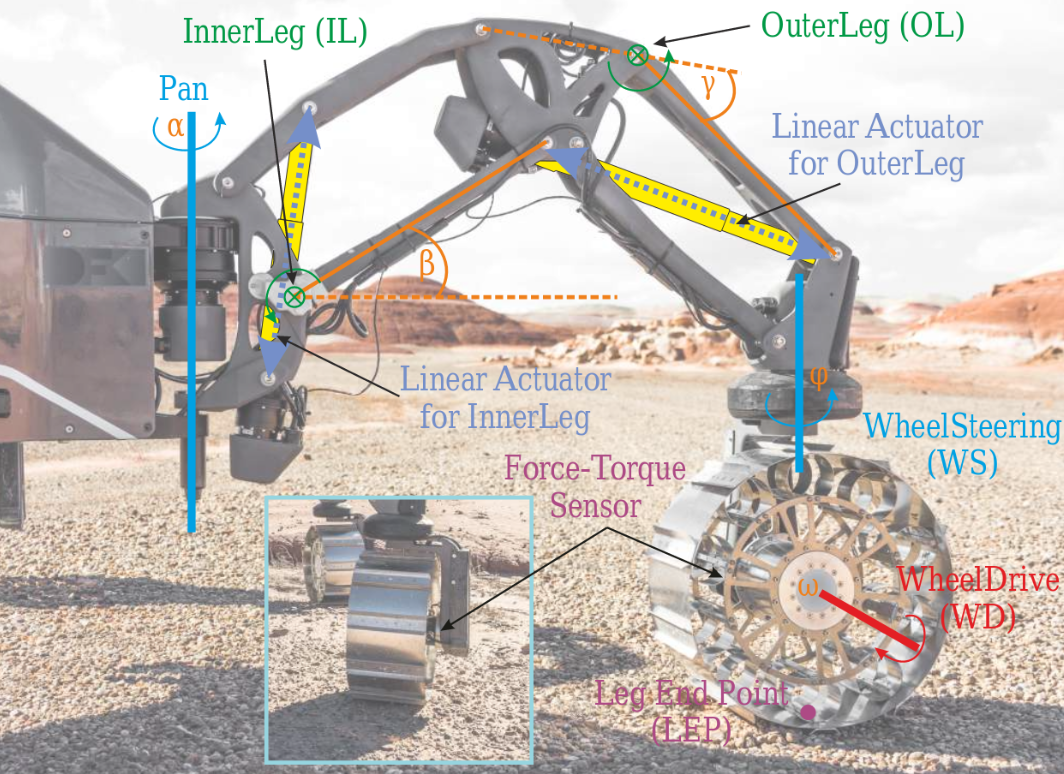
\includegraphics[width=0.8\linewidth]{sections/locomotion-power-draws/images/sherpatt-actively-articulated-suspension-sytem.png}\\
  \caption[SherpaTT actively articulated suspension system]
          {SherpaTT actively articulated suspension system.}
  \label{fig:sherpatt-actively-articulated-suspension-system}
\end{figure}

 This section restricts power draw analysis to establishing propulsion power constraints for the study of SherpaTT Mars mission scenarios. Lack of motor optimisation as well as lower gravity and pressure on Mars permit the assumption that, given similar topology traversals, measured propulsion power draws are greater than those that would be observed on a Martian environment. This assumption is further supported when considering that SherpaTT's velocities during power draw measurements were much greater than what has been achieved on present and past Mars rover missions.


\section{Power Draw}
\label{sec:PropulsionPowerConstraints:PowerDraw}
Available datasets from the Mars analogue field test campaign cover 2 flat surface runs and 3 steep upslope terrain runs. From the 2 upslope runs, the dataset with the worst-case maximum and mean propulsion power draw was used as the worst-case scenario. Hereafter, all mention of SherpaTT power draws will reference measurements included in these datasets. Measured power draws fluctuate due to slips, skids, noise, and other unknown imperfections. To ease readability, local minima, maxima, and media lines have been traced for all power plot figures.


\subsection{Flat Terrain Traverse}
\label{sec:PropulsionPowerConstraints:FlatTerrainTraverse}
\ac{MER} and \ac{MSL} rovers are each equipped with a total of 10 propulsion motors to drive their Rocker-Bogie passive suspension system: 6 to rotate the wheels and 4 to steer them \citeother{Novak2005} \citeother{Lakdawalla2018}. The \ac{MER} rovers needed approximately \SI{100}{\watt} to drive \citeother{MERRoverEnergy}. Propulsion power draws measured for SherpaTT on flat surface runs are shown in Figure \ref{fig:plot:sherpatt-flat-terrain-power-draw}.

\begin{figure}[h]
\captionsetup[subfigure]{justification=centering}
\vspace{-2ex}
	\centering
    %% setup sizes
    \setlength{\subfigureWidth}{0.50\textwidth}
    \setlength{\graphicsHeight}{80mm}
    %% kill hyper-link highlighting
    \hypersetup{hidelinks=true}%
    %% the figures
    \begin{subfigure}[t]{\subfigureWidth}
        \centering
        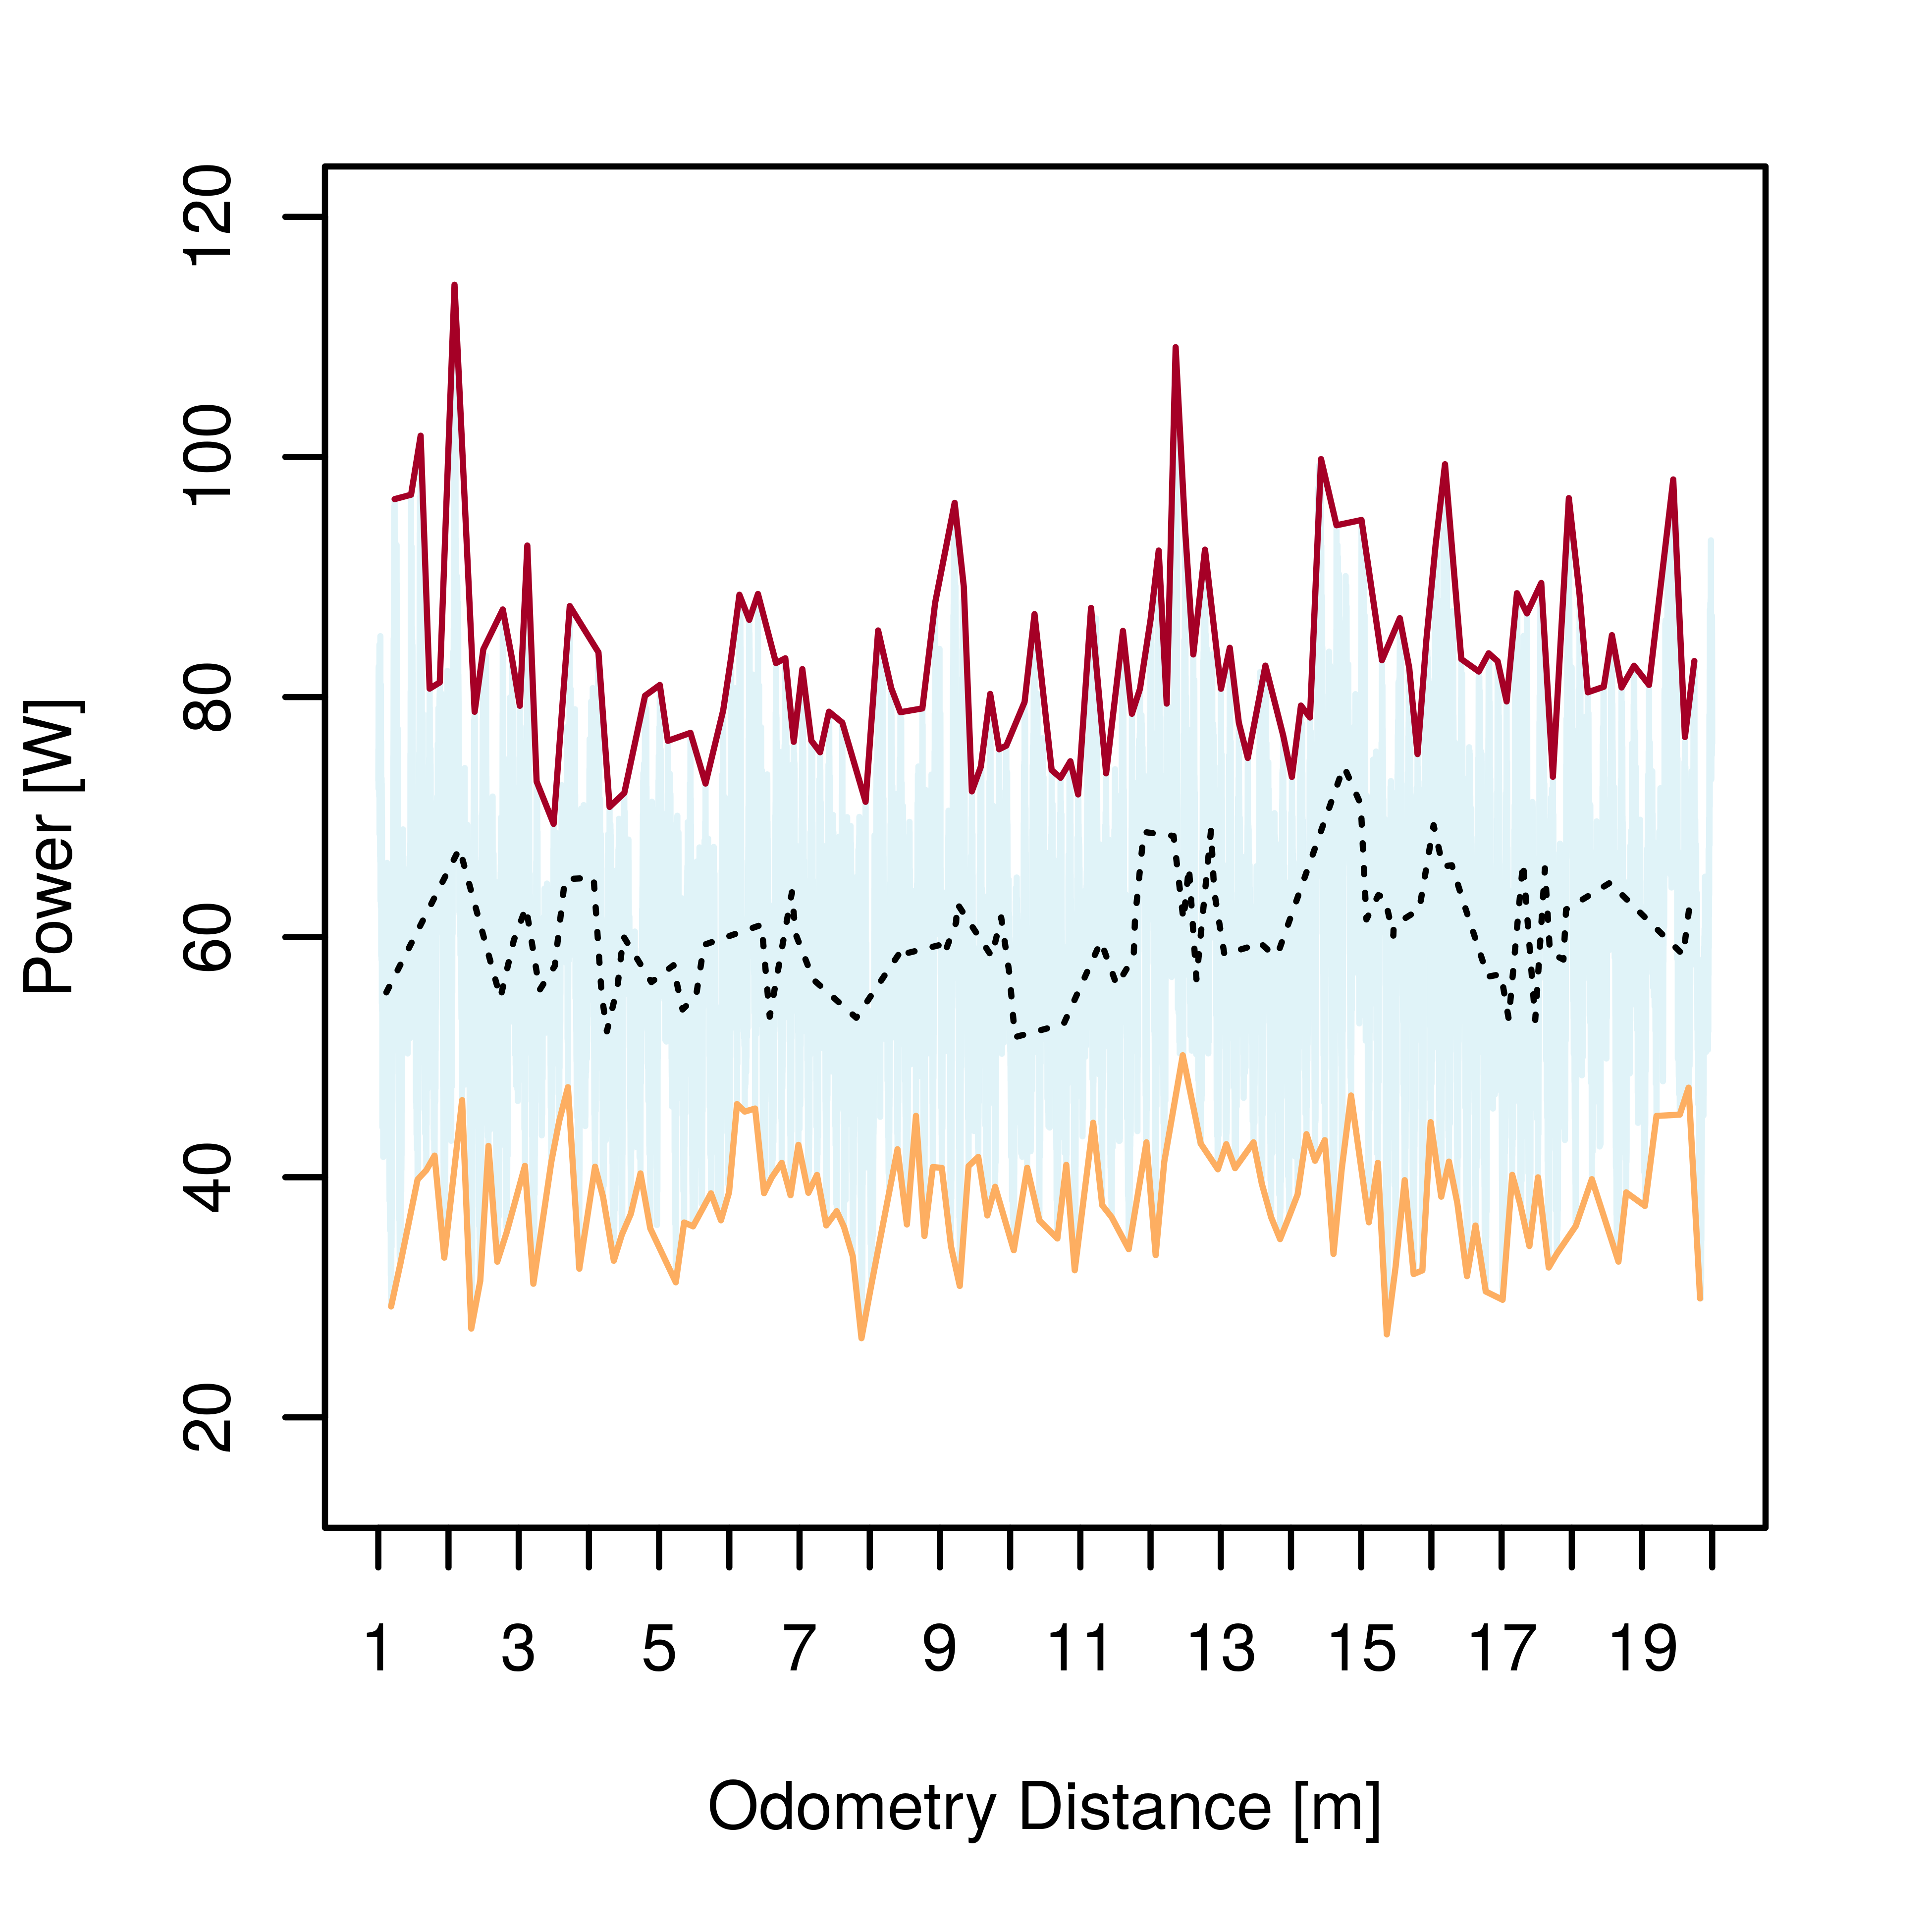
\includegraphics[height=\graphicsHeight]{sections/locomotion-power-draws/plots/locomotion-power-draw-on-flat-terrain-1.png}
        \subcaption{Run \#1}
        \label{fig:plot:sub:sherpatt-flat-terrain-power-draw-1}
    \end{subfigure}\hfill
    \begin{subfigure}[t]{\subfigureWidth}
        \centering
        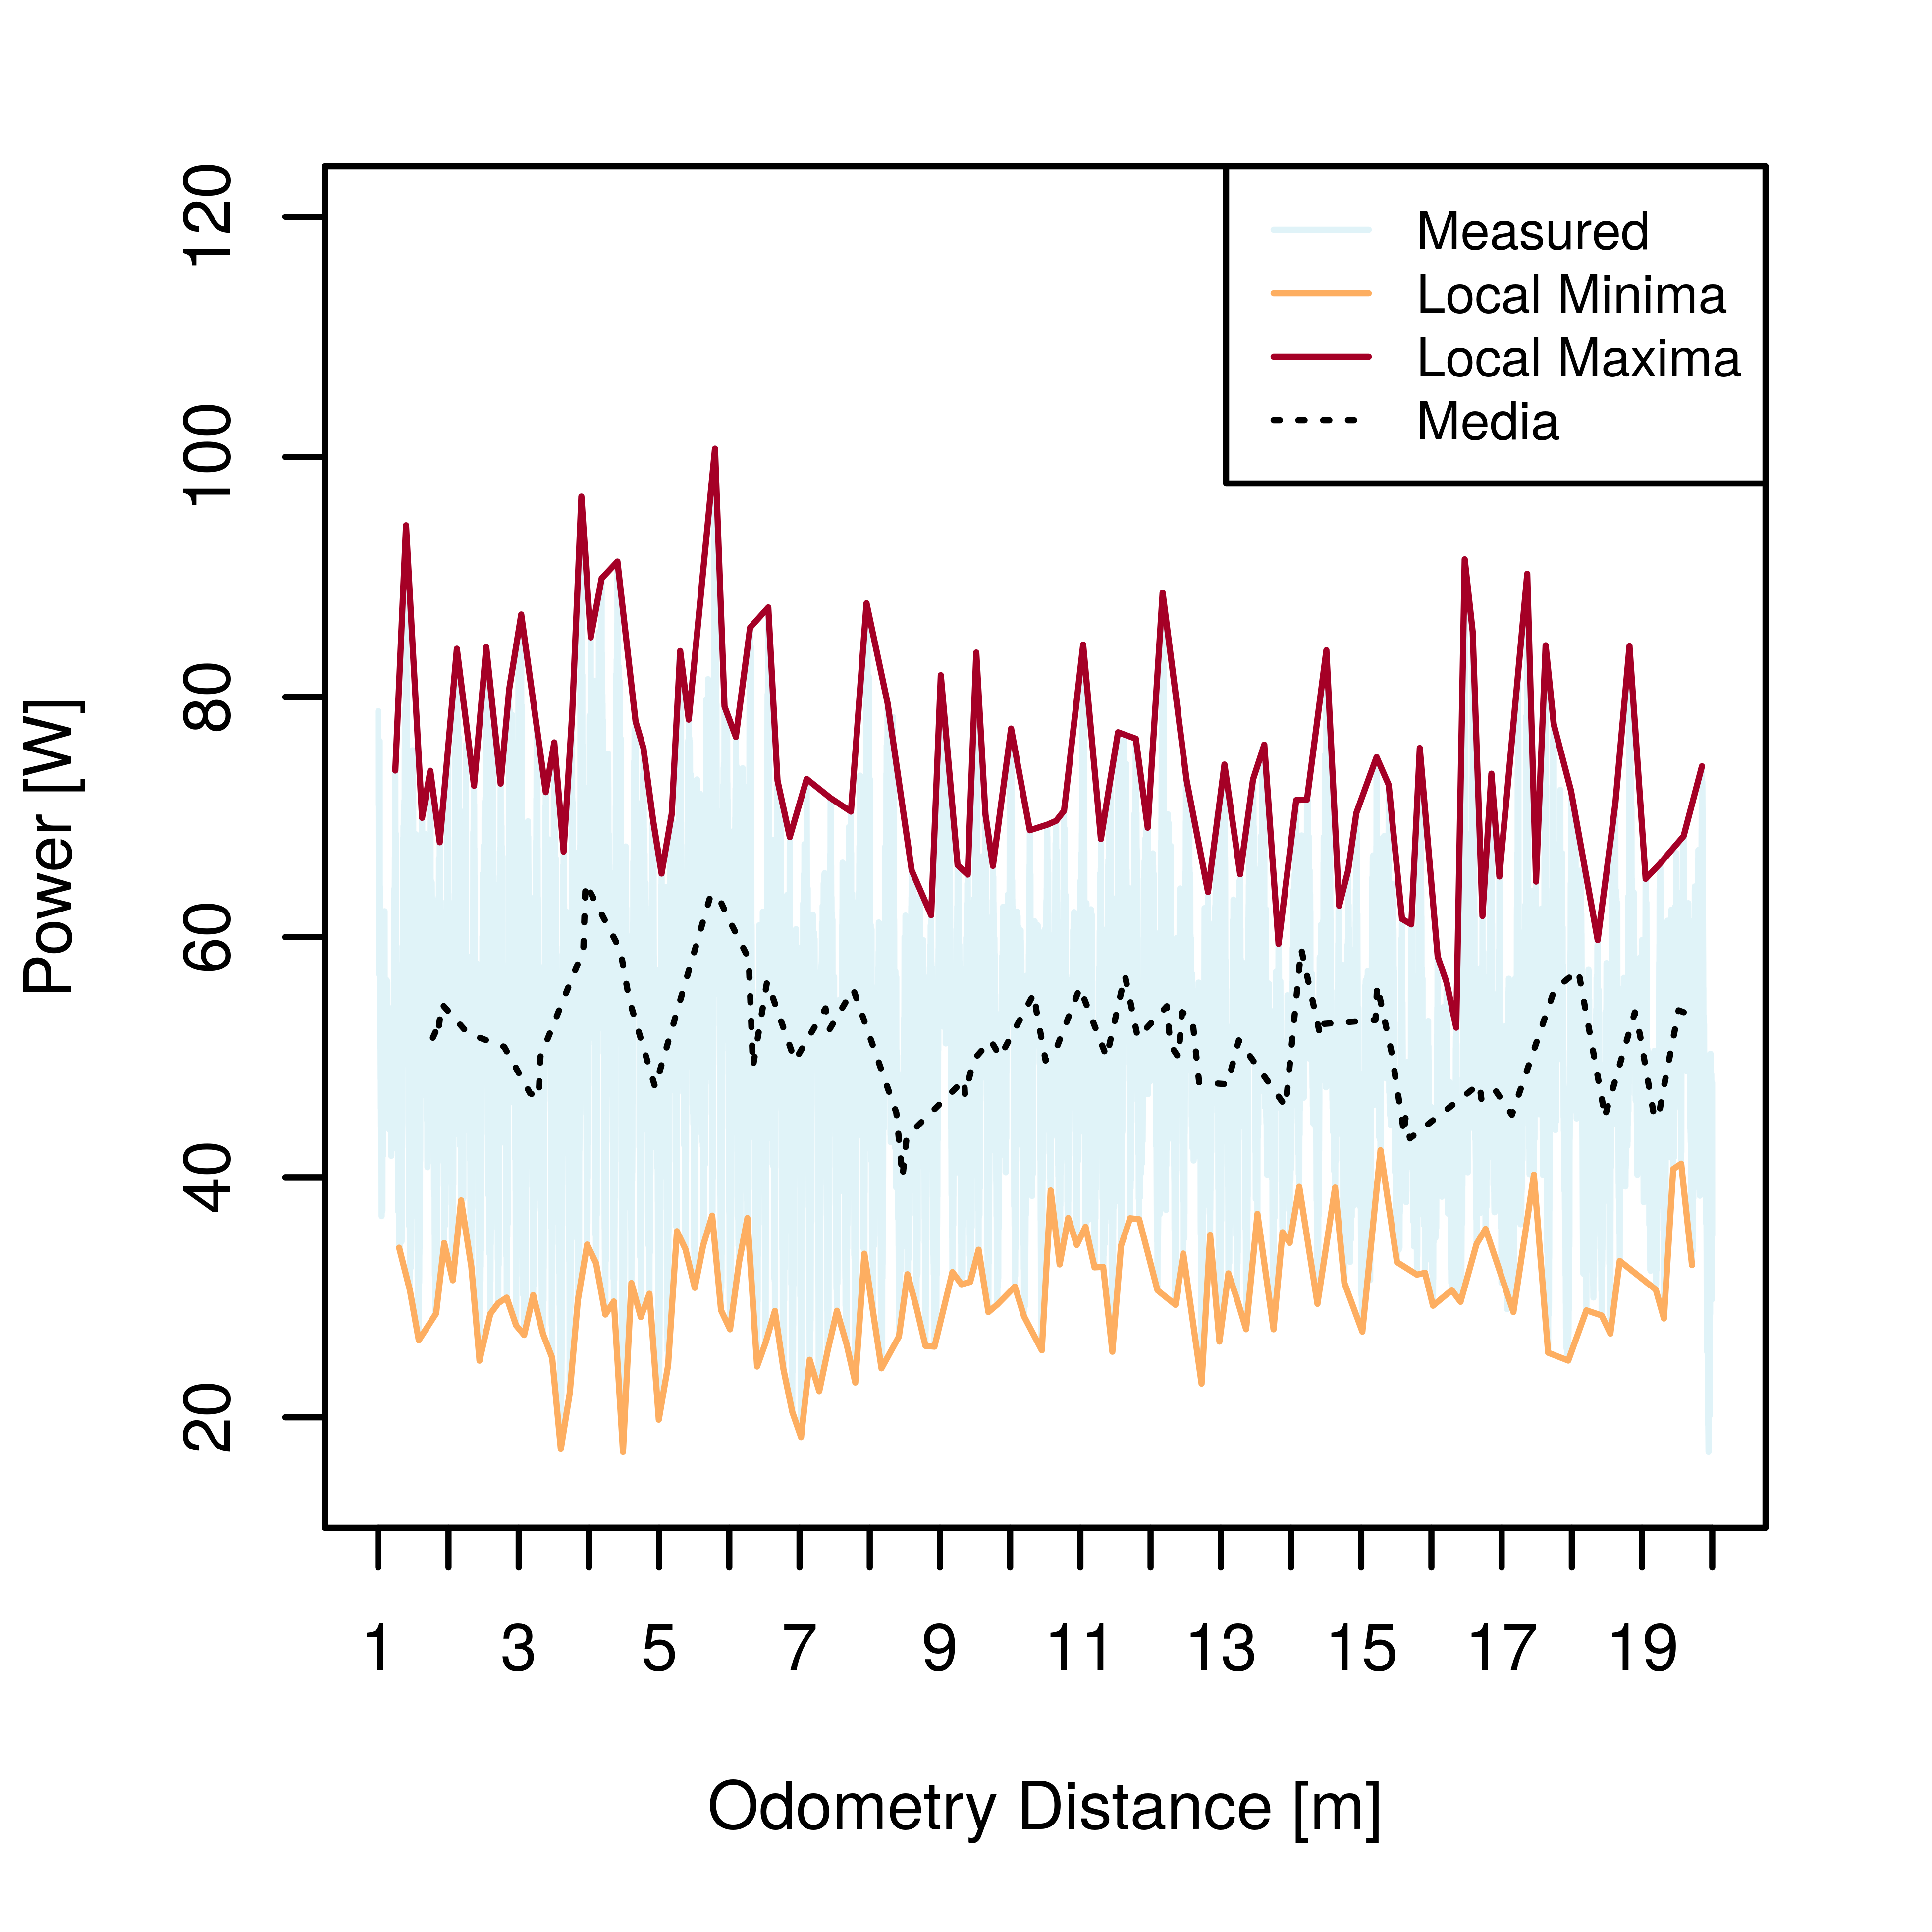
\includegraphics[height=\graphicsHeight]{sections/locomotion-power-draws/plots/locomotion-power-draw-on-flat-terrain-2.png}
  		\subcaption{Run \#2}
		\label{fig:plot:sub:sherpatt-flat-terrain-power-draw-2}
	\end{subfigure}\\[0.8ex]
    \caption[Propulsion power draw for a flat terrain traverse during SherpaTT Mars analogue field tests in Utah]
            {Propulsion power draw for a flat terrain traverse during SherpaTT Mars analogue field tests in Utah.}
    \label{fig:plot:sherpatt-flat-terrain-power-draw}
\vspace{-2ex}
\end{figure}


These measurements are summarised in Table \ref{tab:sherpatt-flat-terrain-global-minimum-maximum-and-medium-power-draws}. To eliminate power draw fluctuations from the analysis, only local media values were considered. Local media were selected rather than the worst-case local maxima on the basis of the assumptions made in Section \ref{sec:PropulsionPowerConstraints:Introduction}. For flat terrain traverses, a worst-case maximum power draw of \SI{74}{\watt} is observed for a mean of \SI{61}{\watt}.

\clearpage
\begin{table}[h]
\centering
\caption{Global minimum, maximum, and medium of traced local minima, maxima, and media for SherpaTT flat terrain propulsion power draw lines.}
\label{tab:sherpatt-flat-terrain-global-minimum-maximum-and-medium-power-draws}
\begin{tabular}{llccc}
\cline{3-5}
\multicolumn{2}{l|}{\multirow{2}{*}{}} & \multicolumn{3}{c|}{\textbf{Power Draw {[}W{]}}} \\ \cline{3-5}
\multicolumn{2}{l|}{} & \multicolumn{1}{c|}{\textbf{\begin{tabular}[c]{@{}c@{}}Global Minimum\end{tabular}}} & \multicolumn{1}{c|}{\textbf{\begin{tabular}[c]{@{}c@{}}Global Maximum\end{tabular}}} & \multicolumn{1}{c|}{\textbf{\begin{tabular}[c]{@{}c@{}}Global Media\end{tabular}}} \\ \hline
\multicolumn{1}{|c|}{\multirow{4}{*}{\textbf{Run \#1}}} & \multicolumn{1}{l|}{\textbf{Measured}} & \multicolumn{1}{c|}{27} & \multicolumn{1}{c|}{114} & \multicolumn{1}{c|}{60} \\ \cline{2-5}
\multicolumn{1}{|c|}{} & \multicolumn{1}{l|}{\textbf{Local Minima}} & \multicolumn{1}{c|}{27} & \multicolumn{1}{c|}{50} & \multicolumn{1}{c|}{38} \\ \cline{2-5}
\multicolumn{1}{|c|}{} & \multicolumn{1}{l|}{\textbf{Local Maxima}} & \multicolumn{1}{c|}{69} & \multicolumn{1}{c|}{114} & \multicolumn{1}{c|}{83} \\ \cline{2-5}
\multicolumn{1}{|c|}{} & \multicolumn{1}{l|}{\textbf{Local Media}} & \multicolumn{1}{c|}{52} & \multicolumn{1}{c|}{74} & \multicolumn{1}{c|}{61} \\ \hhline{|=|=|=|=|=|}
\multicolumn{1}{|l|}{\multirow{4}{*}{\textbf{Run \#2}}} & \multicolumn{1}{l|}{\textbf{Measured}} & \multicolumn{1}{c|}{17} & \multicolumn{1}{c|}{101} & \multicolumn{1}{c|}{51} \\ \cline{2-5}
\multicolumn{1}{|l|}{} & \multicolumn{1}{l|}{\textbf{Local Minima}} & \multicolumn{1}{c|}{17} & \multicolumn{1}{c|}{42} & \multicolumn{1}{c|}{30} \\ \cline{2-5}
\multicolumn{1}{|l|}{} & \multicolumn{1}{l|}{\textbf{Local Maxima}} & \multicolumn{1}{c|}{52} & \multicolumn{1}{c|}{101} & \multicolumn{1}{c|}{74} \\ \cline{2-5}
\multicolumn{1}{|l|}{} & \multicolumn{1}{l|}{\textbf{Local Media}} & \multicolumn{1}{c|}{40} & \multicolumn{1}{c|}{64} & \multicolumn{1}{c|}{52} \\ \hline
 &  & \multicolumn{1}{l}{} & \multicolumn{1}{l}{} & \multicolumn{1}{l}{} \\
 &  & \multicolumn{1}{l}{} & \multicolumn{1}{l}{} & \multicolumn{1}{l}{}
\end{tabular}
\end{table}


\subsection{Upslope Terrain Traverse}
\label{sec:PropulsionPowerConstraints:UpslopeTerrainTraverse}
Propulsion power draws on a steep uplsope were measured along an approximately \SI{16}{\meter} track and are shown Figure \ref{fig:plot:sub:sherpatt-disaggregated-upslope-terrain-power-draw-locomotion}. The drive and suspension power draw components are shown in Figures \ref{fig:plot:sub:sherpatt-disaggregated-upslope-terrain-power-draw-drive} and \ref{fig:plot:sub:sherpatt-disaggregated-upslope-terrain-power-draw-suspension}, respectively.

\begin{figure}[h]
\captionsetup[subfigure]{justification=centering}
\vspace{-2ex}
	\centering
    %% setup sizes
    \setlength{\subfigureWidth}{0.32\textwidth}
    \setlength{\graphicsHeight}{50mm}
    %% kill hyper-link highlighting
    \hypersetup{hidelinks=true}%
    %% the figures
	\begin{subfigure}[t]{\subfigureWidth}
        \centering
        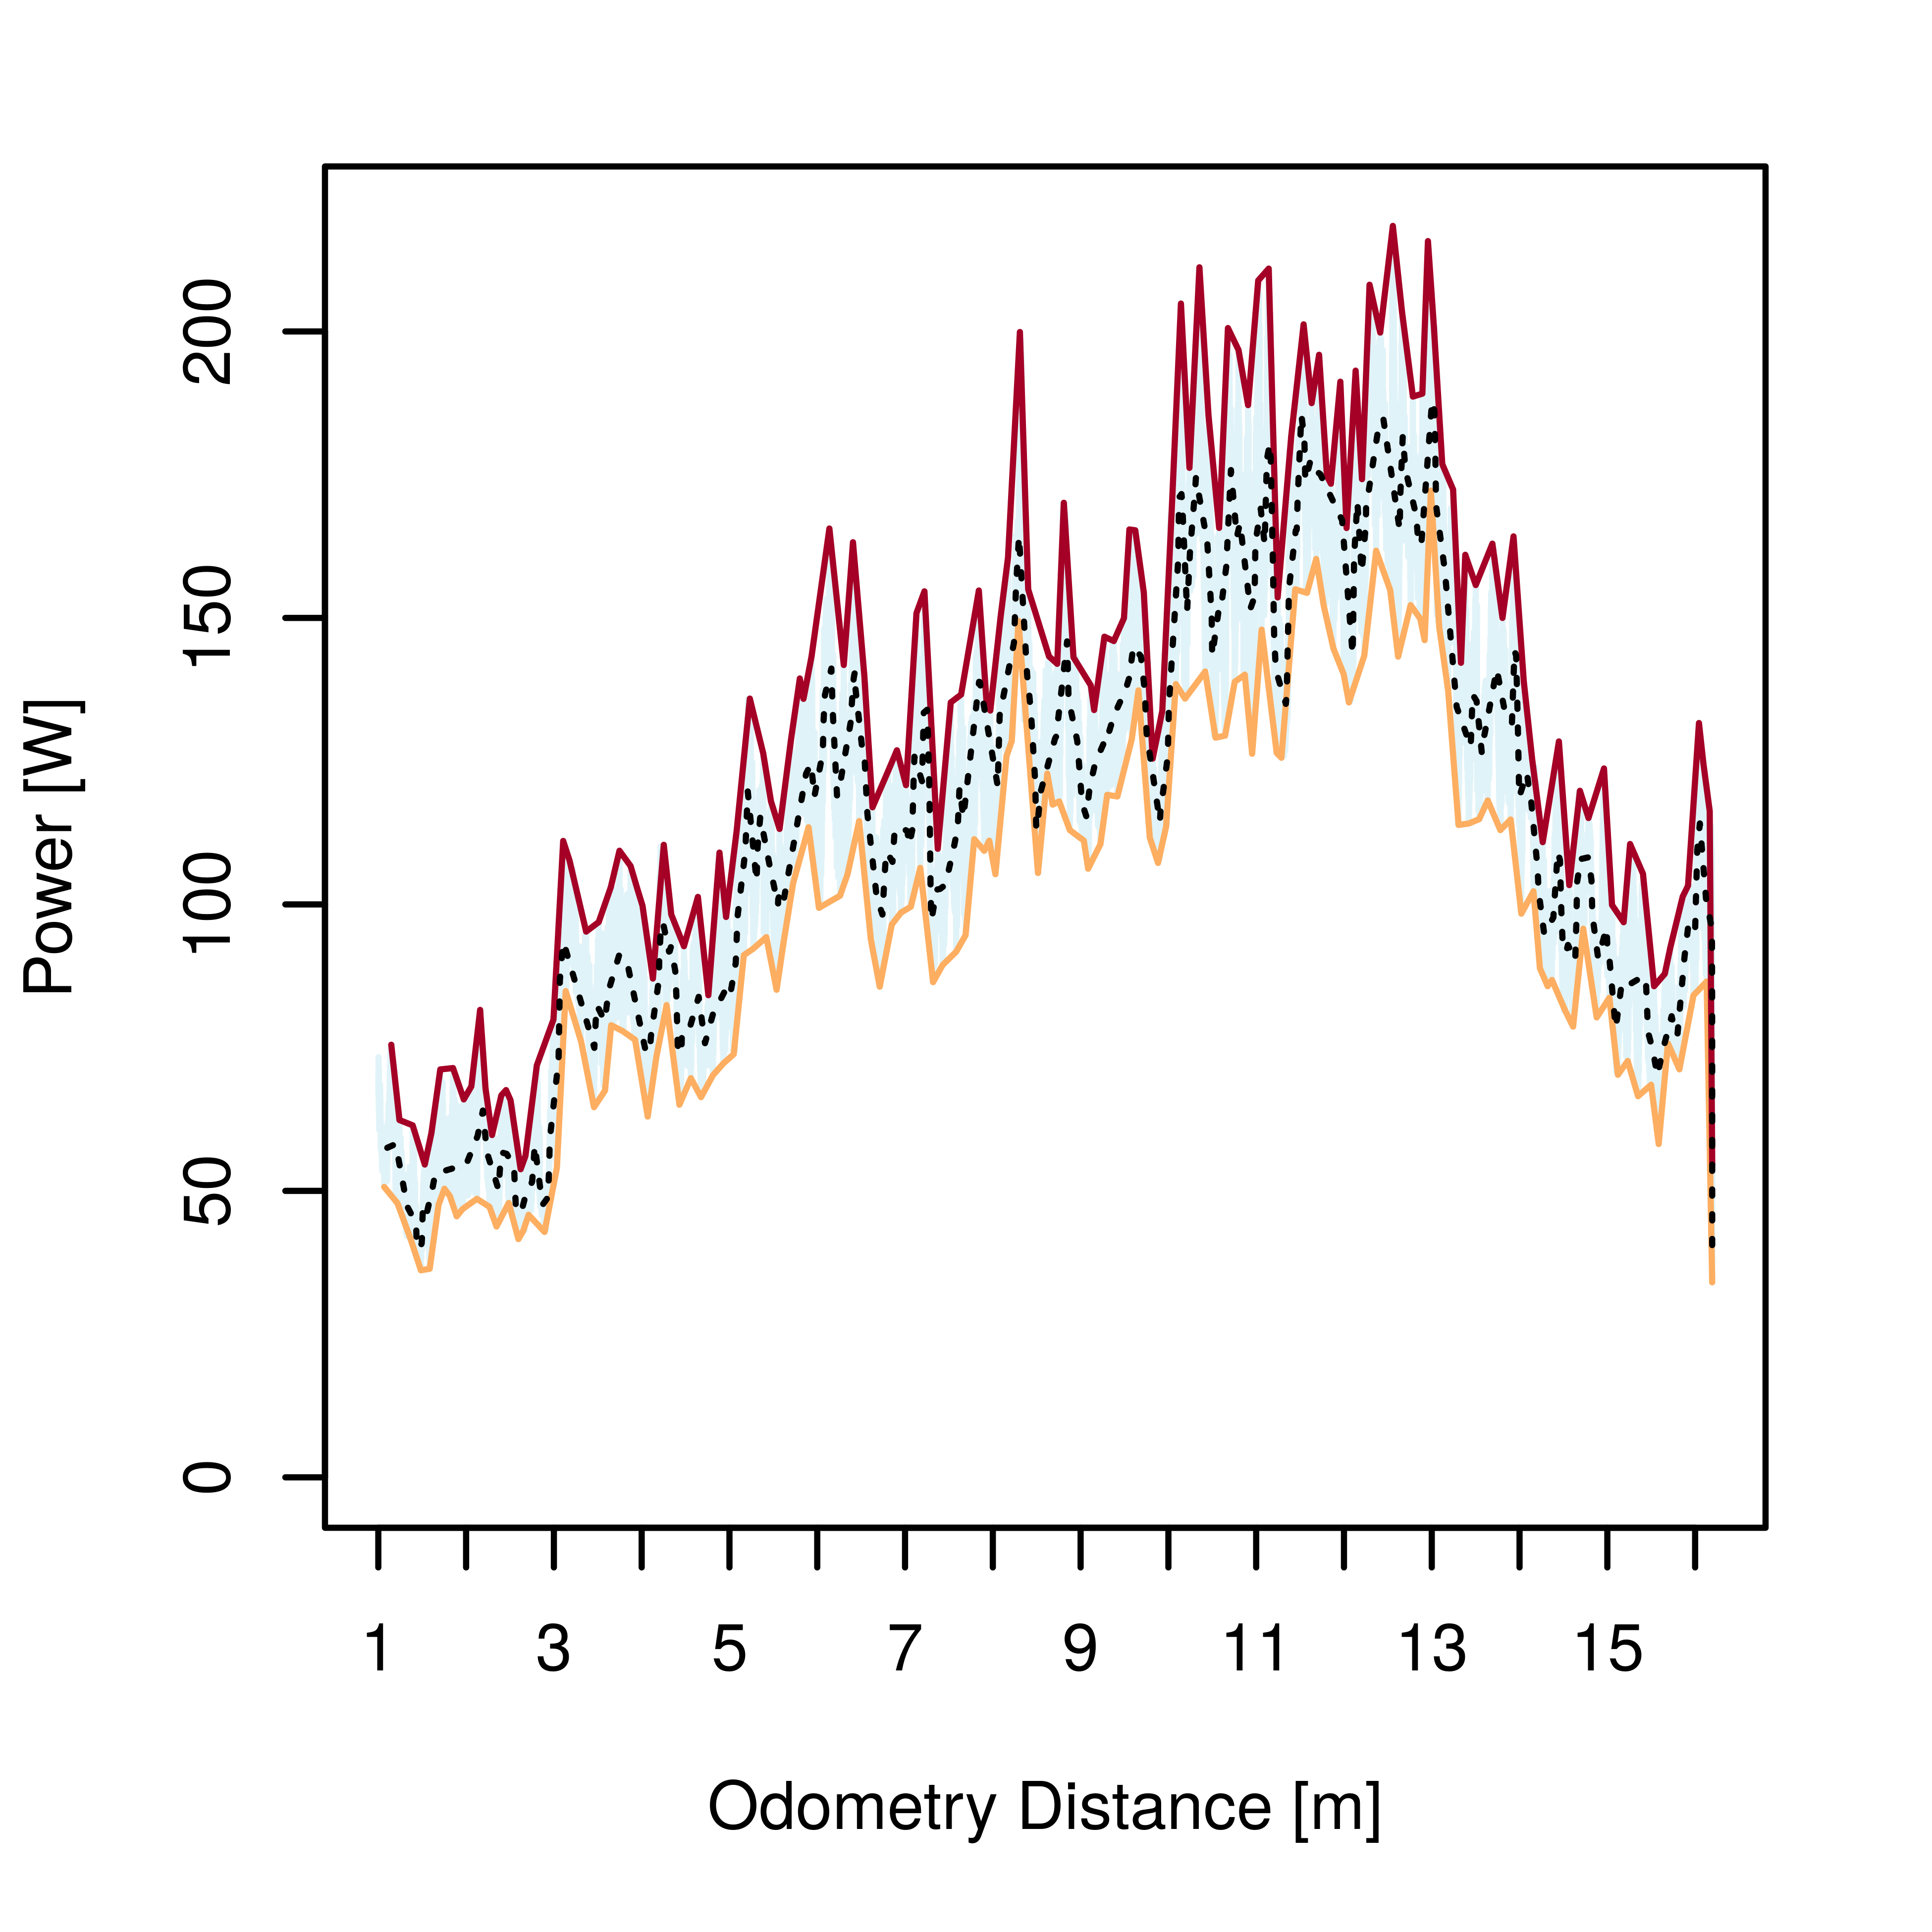
\includegraphics[height=\graphicsHeight]{sections/locomotion-power-draws/plots/locomotion-power-draw-on-upslope-terrain.png}
  		\subcaption{Propulsion}
		\label{fig:plot:sub:sherpatt-disaggregated-upslope-terrain-power-draw-locomotion}
	\end{subfigure}\hfill
	\begin{subfigure}[t]{\subfigureWidth}
        \centering
        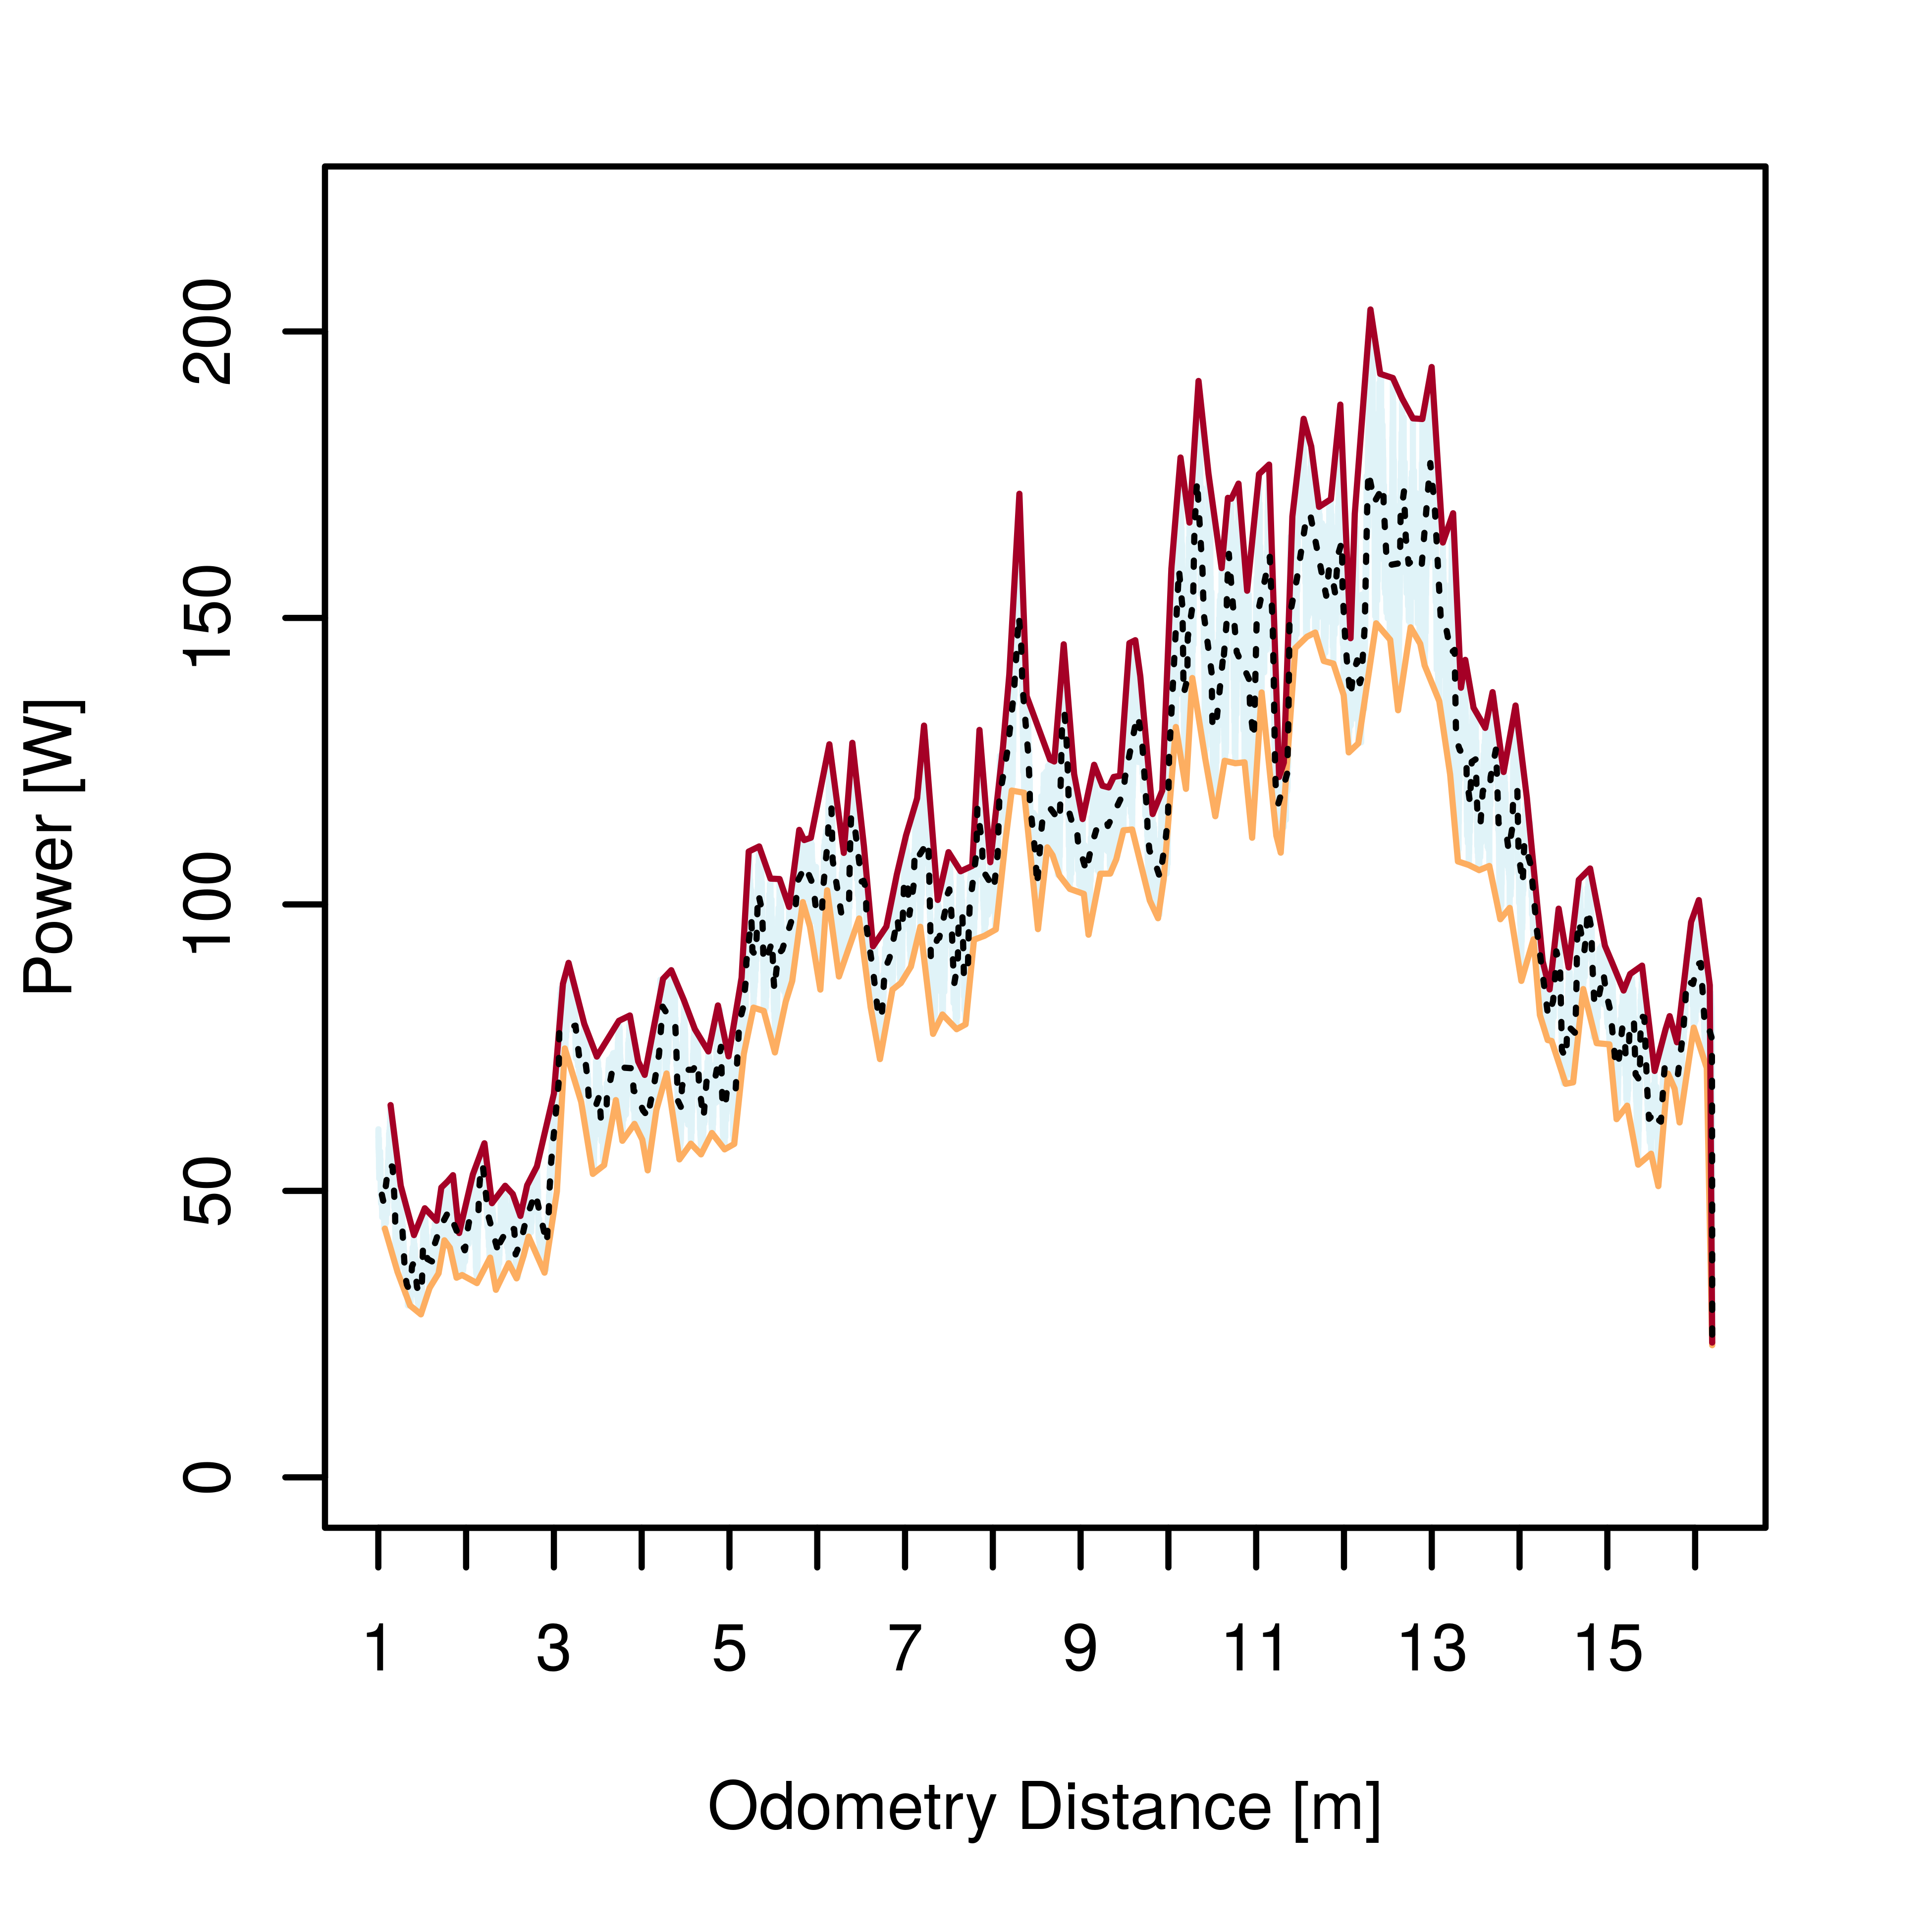
\includegraphics[height=\graphicsHeight]{sections/locomotion-power-draws/plots/drive-power-draw-on-upslope-terrain.png}
  		\subcaption{Drive}
		\label{fig:plot:sub:sherpatt-disaggregated-upslope-terrain-power-draw-drive}
	\end{subfigure}\hfill
    \begin{subfigure}[t]{\subfigureWidth}
        \centering
        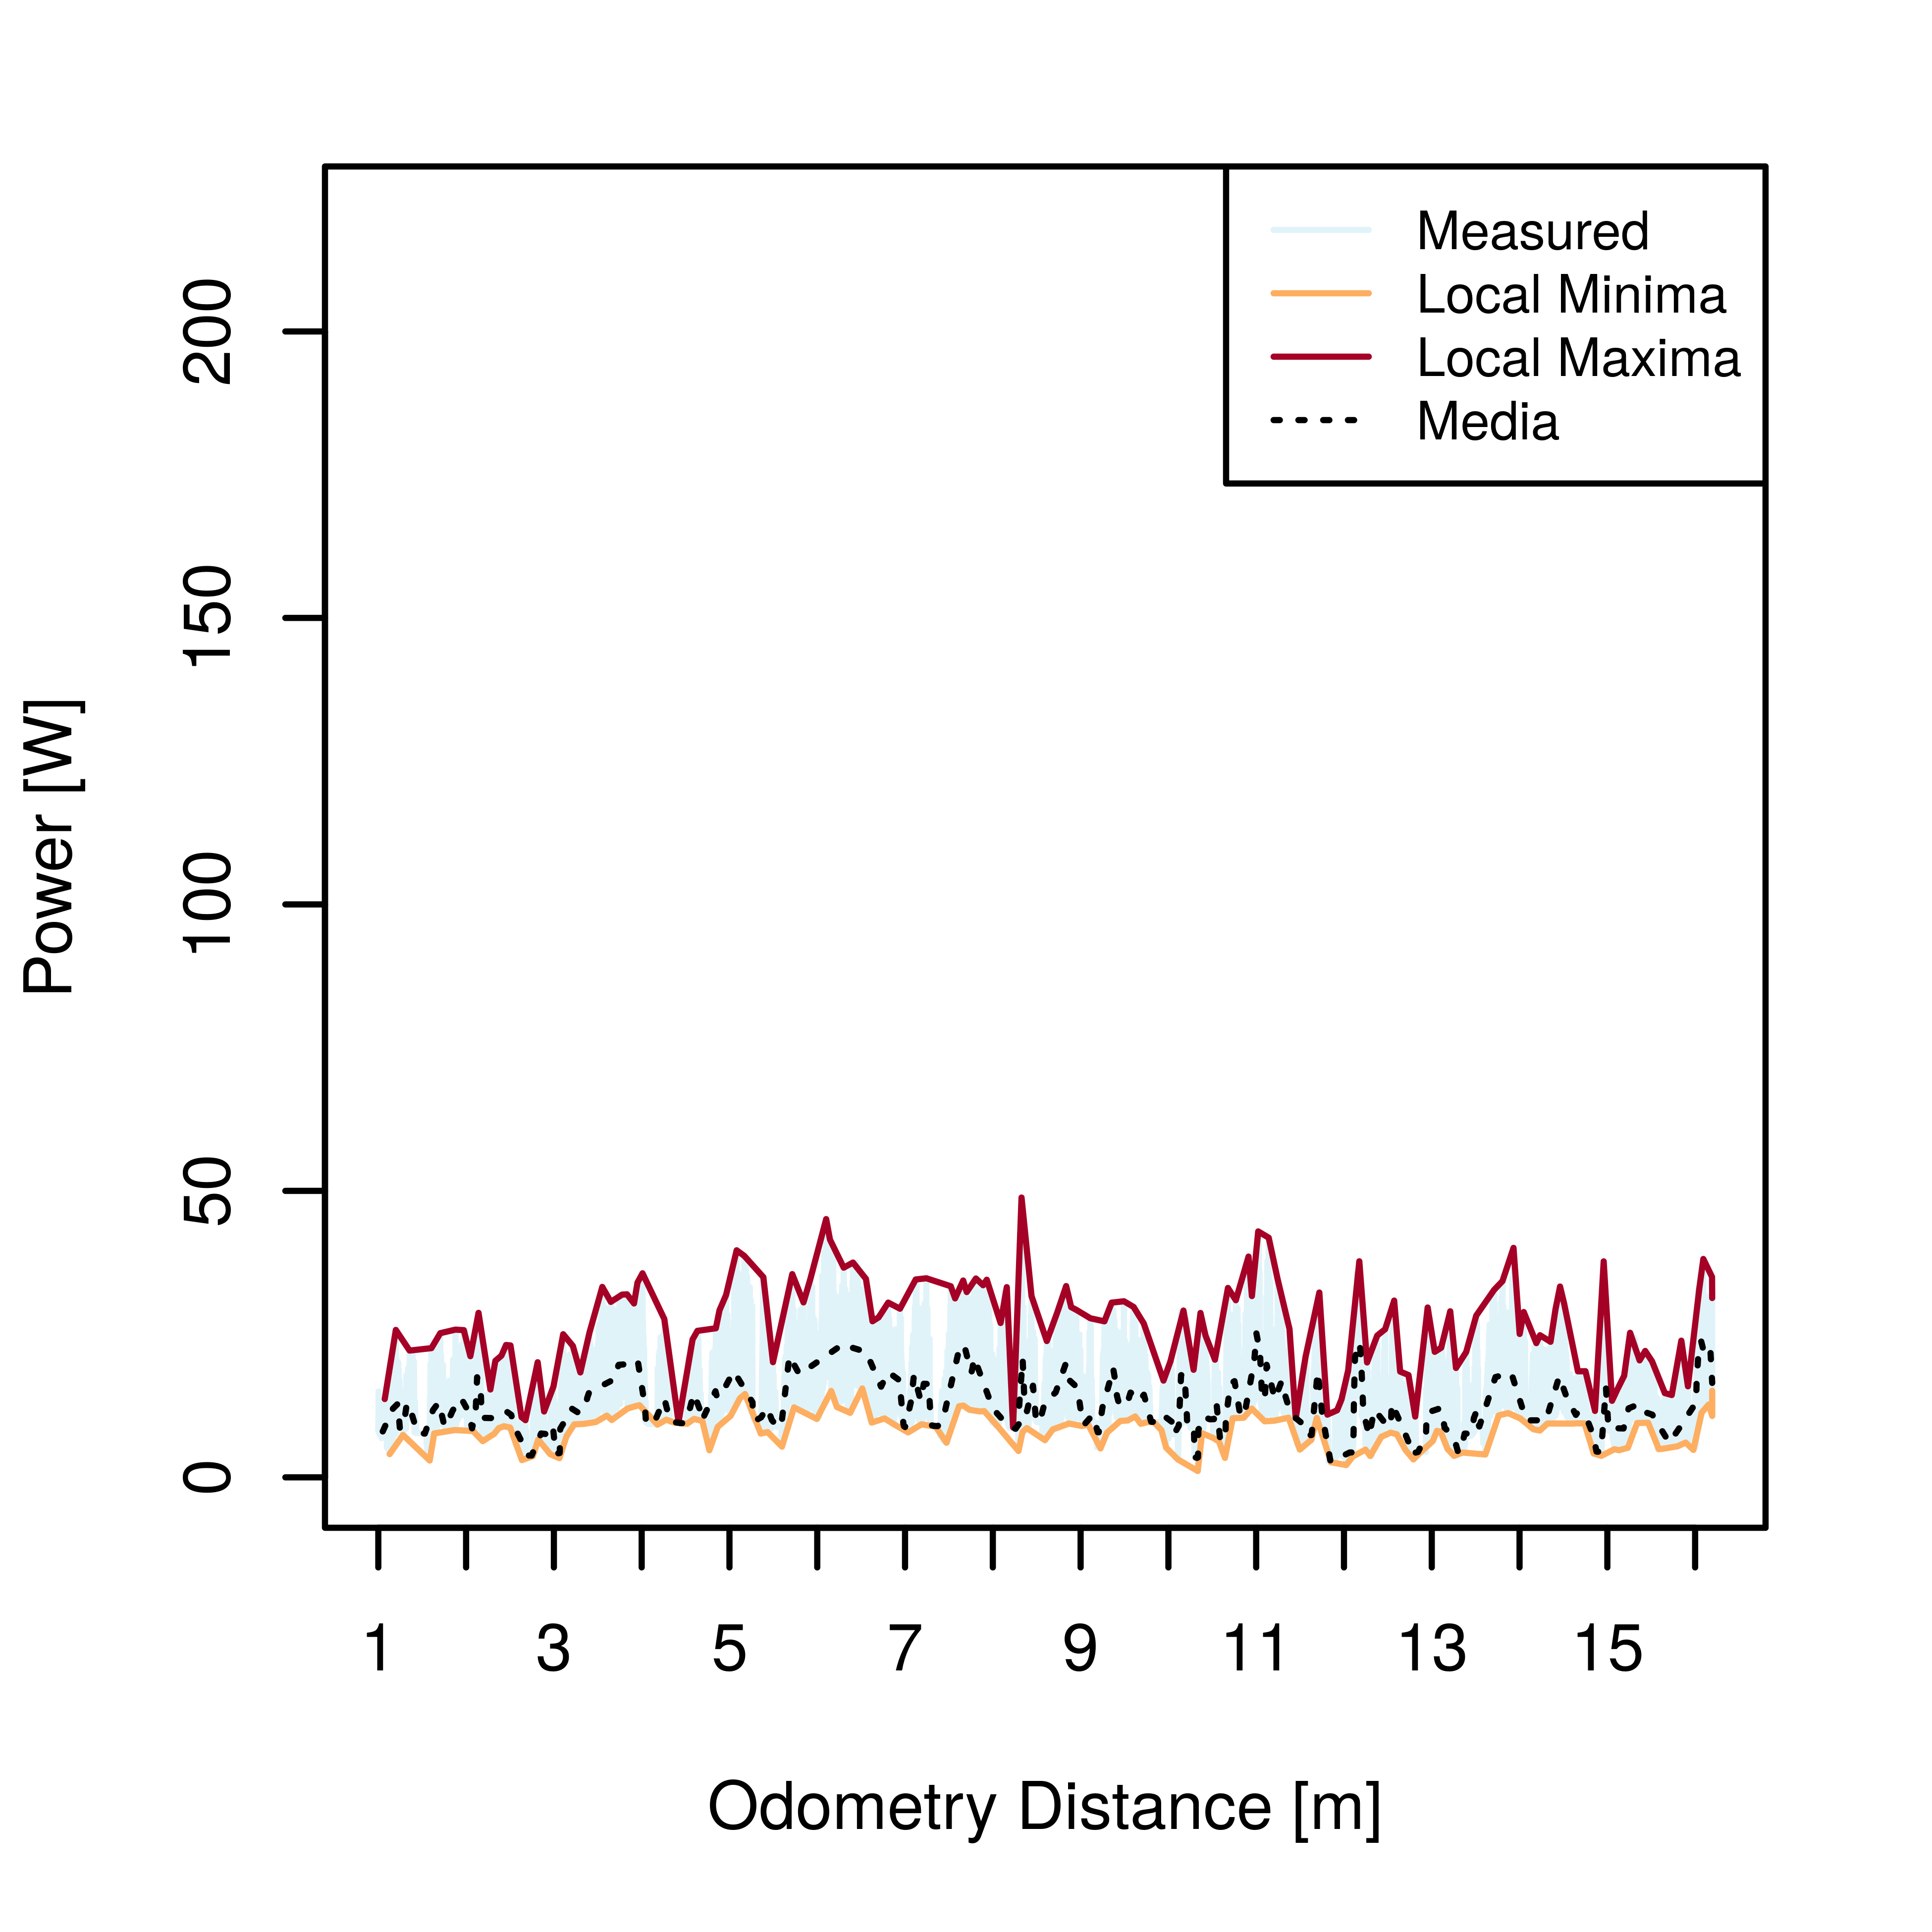
\includegraphics[height=\graphicsHeight]{sections/locomotion-power-draws/plots/suspension-power-draw-on-upslope-terrain.png}
  		\subcaption{Suspension}
		\label{fig:plot:sub:sherpatt-disaggregated-upslope-terrain-power-draw-suspension}
	\end{subfigure}\\[0.8ex]
    \caption[Disaggregated measurements of power draw for upslope terrain traverse during SherpaTT Mars analogue field tests in Utah]
            {Disaggregated measurements of power draw for upslope terrain traverse during SherpaTT Mars analogue field tests in Utah.}
    \label{fig:plot:sherpatt-disaggregated-upslope-terrain-power-draw}
\vspace{-2ex}
\end{figure}

An uplsope traverse has no discernable effect on the suspension power draw, however; there is a clear gradual increase in the drive power draw. The global maximum, minimum, and medium of the traced local minima, maxima, and media power draw lines are presented in Table \ref{tab:sherpatt-upslope-terrain-global-minimum-maximum-and-medium-power-draws}.

\clearpage
\begin{table}[h]
\centering
\caption{Global minimum, maximum, and medium of traced local minima, maxima, and media for SherpaTT upslope terrain traverse propulsion power draw lines.}
\label{tab:sherpatt-upslope-terrain-global-minimum-maximum-and-medium-power-draws}
\begin{tabular}{l|c|c|c|}
\cline{2-4}
\multicolumn{1}{c|}{\multirow{2}{*}{\textbf{}}} & \multicolumn{3}{c|}{\textbf{Power Draw {[}W{]}}} \\ \cline{2-4}
\multicolumn{1}{c|}{} & \textbf{\begin{tabular}[c]{@{}c@{}}Global Minimum\end{tabular}} & \textbf{\begin{tabular}[c]{@{}c@{}}Global Maximum\end{tabular}} & \textbf{\begin{tabular}[c]{@{}c@{}}Global Media\end{tabular}} \\ \hline
\multicolumn{1}{|l|}{\textbf{Measured}} & 34 & 218 & 114 \\ \hline
\multicolumn{1}{|l|}{\textbf{Local Minima}} & 34 & 172 & 98 \\ \hline
\multicolumn{1}{|l|}{\textbf{Local Maxima}} & 54 & 218 & 133 \\ \hline
\multicolumn{1}{|l|}{\textbf{Local Media}} & 40 & 188 & 18 \\ \hline
\end{tabular}
\end{table}


Figure \ref{fig:plot:sherpatt-upslope-terrain-power-draw} overlaps the propulsion local media power draws with the tackled slope angles. The steepest slope angle was \SI{28}{\degree} for an average of \SI{17.52}{\degree}. Slope angle increase are consistently followed by power draw spikes, i.e. at approximately 3, 4, 5, 6, 8, and 9 meters in the odometry measurements. Inversely, slope angle decreases were followed by power draws troughs at approximately 11, 13, 14, and 16 meters.

\begin{figure}[h]
  \centering
  \hypersetup{linkcolor=captionTextColor}
  \includegraphics[width=0.8\linewidth]{sections/locomotion-power-draws/plots/minima-locomotion-power-draws-on-upslope-terrain.png}\\
  \caption[Mean Propulsion power draw for an upslope terrain traverse during SherpaTT Utah field test campaign.]
          {Mean Propulsion power draw for an upslope terrain traverse during SherpaTT Utah field test campaign.}
  \label{fig:plot:sherpatt-upslope-terrain-power-draw}
\end{figure}

The power draws trough following the slope angle change from \SI{28}{\degree} to \SI{20}{\degree} at the \SI{11}{\meter} mark is subsequently followed by an unusual power draw increase and fluctuation. These measurements were discarded as they are outliers with respect to the power draw responses for the slope angle descreases that followed.

Table \ref{tab:sherpatt-upslope-terrain-local-media-measurement-summary} summarises the minimum, maximum, and mean local media propulsion power draws that were measured for different slope angles. Discarding the outlier measurements subsequent to the slope angle change from \SI{28}{\degree} to \SI{20}{\degree} at the \SI{11}{\meter} to \SI{13}{\meter} portion of the track, the maximum mean local media propulsion power draw is \SI{146}{\watt}.

\clearpage
\begin{table}[h]
\centering
\caption{SherpaTT mean propulsion power draw measurements for different slope sections}
\label{tab:sherpatt-upslope-terrain-local-media-measurement-summary}
\begin{tabular}{cc|c|c|c|}
\cline{3-5}
\multicolumn{1}{l}{} & \multicolumn{1}{l|}{} & \multicolumn{3}{c|}{\textbf{Power {[}W{]}}} \\ \hline
\multicolumn{1}{|l|}{\textbf{Distance {[}m{]}}} & \multicolumn{1}{l|}{\textbf{Slope Angle {[}deg{]}}} & \multicolumn{1}{l|}{\textbf{Minimum}} & \multicolumn{1}{l|}{\textbf{Maximum}} & \multicolumn{1}{l|}{\textbf{Mean}} \\ \hline
\multicolumn{1}{|c|}{\textbf{1 $<$ x $\leq$ 3}} & 10 & 40 & 64 & 51 \\ \hline
\multicolumn{1}{|c|}{\textbf{3 $<$ x $\leq$ 4}} & 11 & 73 & 93 & 85 \\ \hline
\multicolumn{1}{|c|}{\textbf{4 $<$ x $\leq$ 5}} & 15 & 74 & 87 & 83 \\ \hline
\multicolumn{1}{|c|}{\textbf{5 $<$ x $\leq$ 6}} & 16 & 85 & 125 & 107 \\ \hline
\multicolumn{1}{|c|}{\textbf{6 $<$ x $\leq$ 7}} & 28 & 98 & 141 & 123 \\ \hline
\multicolumn{1}{|c|}{\textbf{7 $<$ x $\leq$ 8}} & 22 & 97 & 139 & 116 \\ \hline
\multicolumn{1}{|c|}{\textbf{8 $<$ x $\leq$ 9}} & 25 & 113 & 164 & 133 \\ \hline
\multicolumn{1}{|c|}{\textbf{9 $<$ x $\leq$ 11}} & 28 & 114 & 176 & 146 \\ \hline
\multicolumn{1}{|c|}{\textbf{11 $<$ x $\leq$ 13}} & 20 & 135 & 188 & 167 \\ \hline
\multicolumn{1}{|c|}{\textbf{13 $<$ x $\leq$ 14}} & 15 & 119 & 123 & 145 \\ \hline
\multicolumn{1}{|c|}{\textbf{14 $<$ x $\leq$ 16}} & 10 & 70 & 186 & 94 \\ \hline
\end{tabular}
\end{table}


\section{Conclusion}
\label{sec:PropulsionPowerConstraints:Conclusion}
Based on data from the SherpaTT field campaign and the assumptions made in Section \ref{sec:PropulsionPowerConstraints:Introduction}, the following power subsystem requirements were proposed with respect to propulsion power draws:

\begin{itemize}
    \item The rover shall provide up to \SI{75}{\watt} in propulsion power for flat terrain traverses.
    \item The rover shall provide up to \SI{150}{\watt} in propulsion power for upslope terrain traverses of up to \SI{30}{\degree} inclination.
\end{itemize}


\clearpage
\section{Power Budget}
\label{sec:Design:PowerBudget}
\section{Introduction}
\label{sec:PropulsionPowerConstraints:Introduction}
SherpaTT's actively articulated suspension system consists of 4 wheeled-legs with a total of 20 motors. Each leg is equipped with 3 suspension motors and 2 drive motors. The suspension motors are responsible for Pan, \ac{IL}, and \ac{OL} revolute joint rotations whereas the drive motors are responsible for \ac{WS} and \ac{WD}. The distribution of these motors across each leg are shown in Figure \ref{fig:sherpatt-actively-articulated-suspension-system}. Propulsion power draw refers to the summation of suspension and drive motor power draws. These power draws have been studied in detail for SherpaTT during a Mars analogue field campaign in Utah \citeother{Cordes2018}.

\begin{figure}[h]
  \centering
  \hypersetup{linkcolor=captionTextColor}
  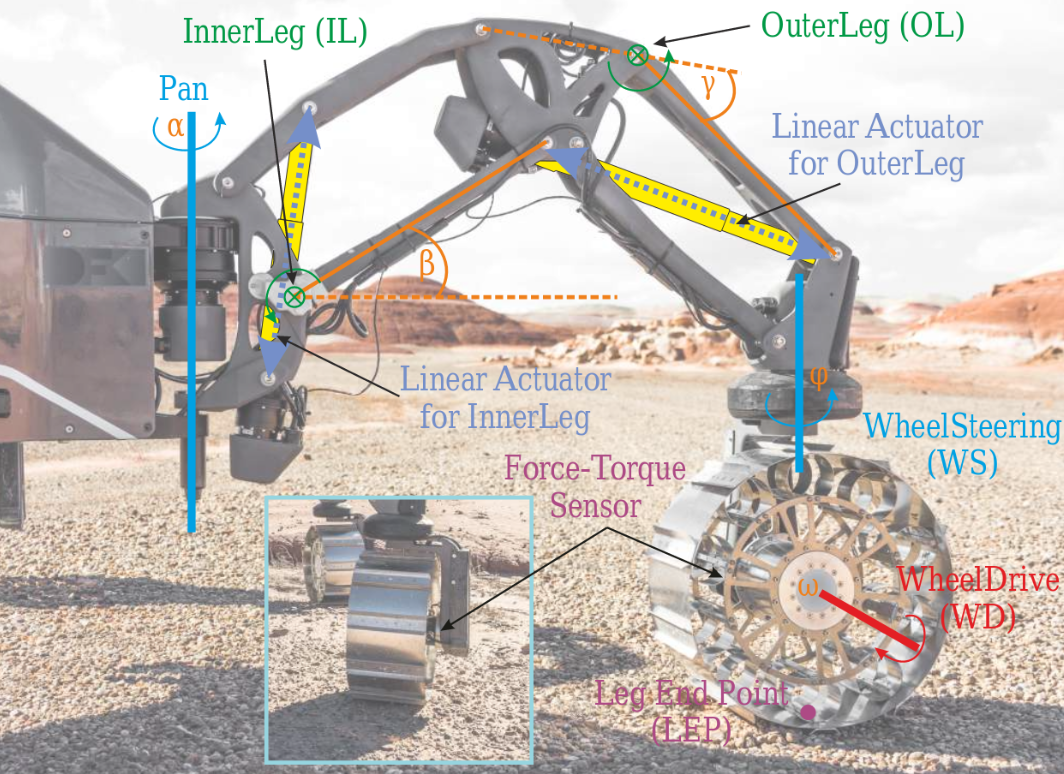
\includegraphics[width=0.8\linewidth]{sections/locomotion-power-draws/images/sherpatt-actively-articulated-suspension-sytem.png}\\
  \caption[SherpaTT actively articulated suspension system]
          {SherpaTT actively articulated suspension system.}
  \label{fig:sherpatt-actively-articulated-suspension-system}
\end{figure}

 This section restricts power draw analysis to establishing propulsion power constraints for the study of SherpaTT Mars mission scenarios. Lack of motor optimisation as well as lower gravity and pressure on Mars permit the assumption that, given similar topology traversals, measured propulsion power draws are greater than those that would be observed on a Martian environment. This assumption is further supported when considering that SherpaTT's velocities during power draw measurements were much greater than what has been achieved on present and past Mars rover missions.


\section{Power Draw}
\label{sec:PropulsionPowerConstraints:PowerDraw}
Available datasets from the Mars analogue field test campaign cover 2 flat surface runs and 3 steep upslope terrain runs. From the 2 upslope runs, the dataset with the worst-case maximum and mean propulsion power draw was used as the worst-case scenario. Hereafter, all mention of SherpaTT power draws will reference measurements included in these datasets. Measured power draws fluctuate due to slips, skids, noise, and other unknown imperfections. To ease readability, local minima, maxima, and media lines have been traced for all power plot figures.


\subsection{Flat Terrain Traverse}
\label{sec:PropulsionPowerConstraints:FlatTerrainTraverse}
\ac{MER} and \ac{MSL} rovers are each equipped with a total of 10 propulsion motors to drive their Rocker-Bogie passive suspension system: 6 to rotate the wheels and 4 to steer them \citeother{Novak2005} \citeother{Lakdawalla2018}. The \ac{MER} rovers needed approximately \SI{100}{\watt} to drive \citeother{MERRoverEnergy}. Propulsion power draws measured for SherpaTT on flat surface runs are shown in Figure \ref{fig:plot:sherpatt-flat-terrain-power-draw}.

\begin{figure}[h]
\captionsetup[subfigure]{justification=centering}
\vspace{-2ex}
	\centering
    %% setup sizes
    \setlength{\subfigureWidth}{0.50\textwidth}
    \setlength{\graphicsHeight}{80mm}
    %% kill hyper-link highlighting
    \hypersetup{hidelinks=true}%
    %% the figures
    \begin{subfigure}[t]{\subfigureWidth}
        \centering
        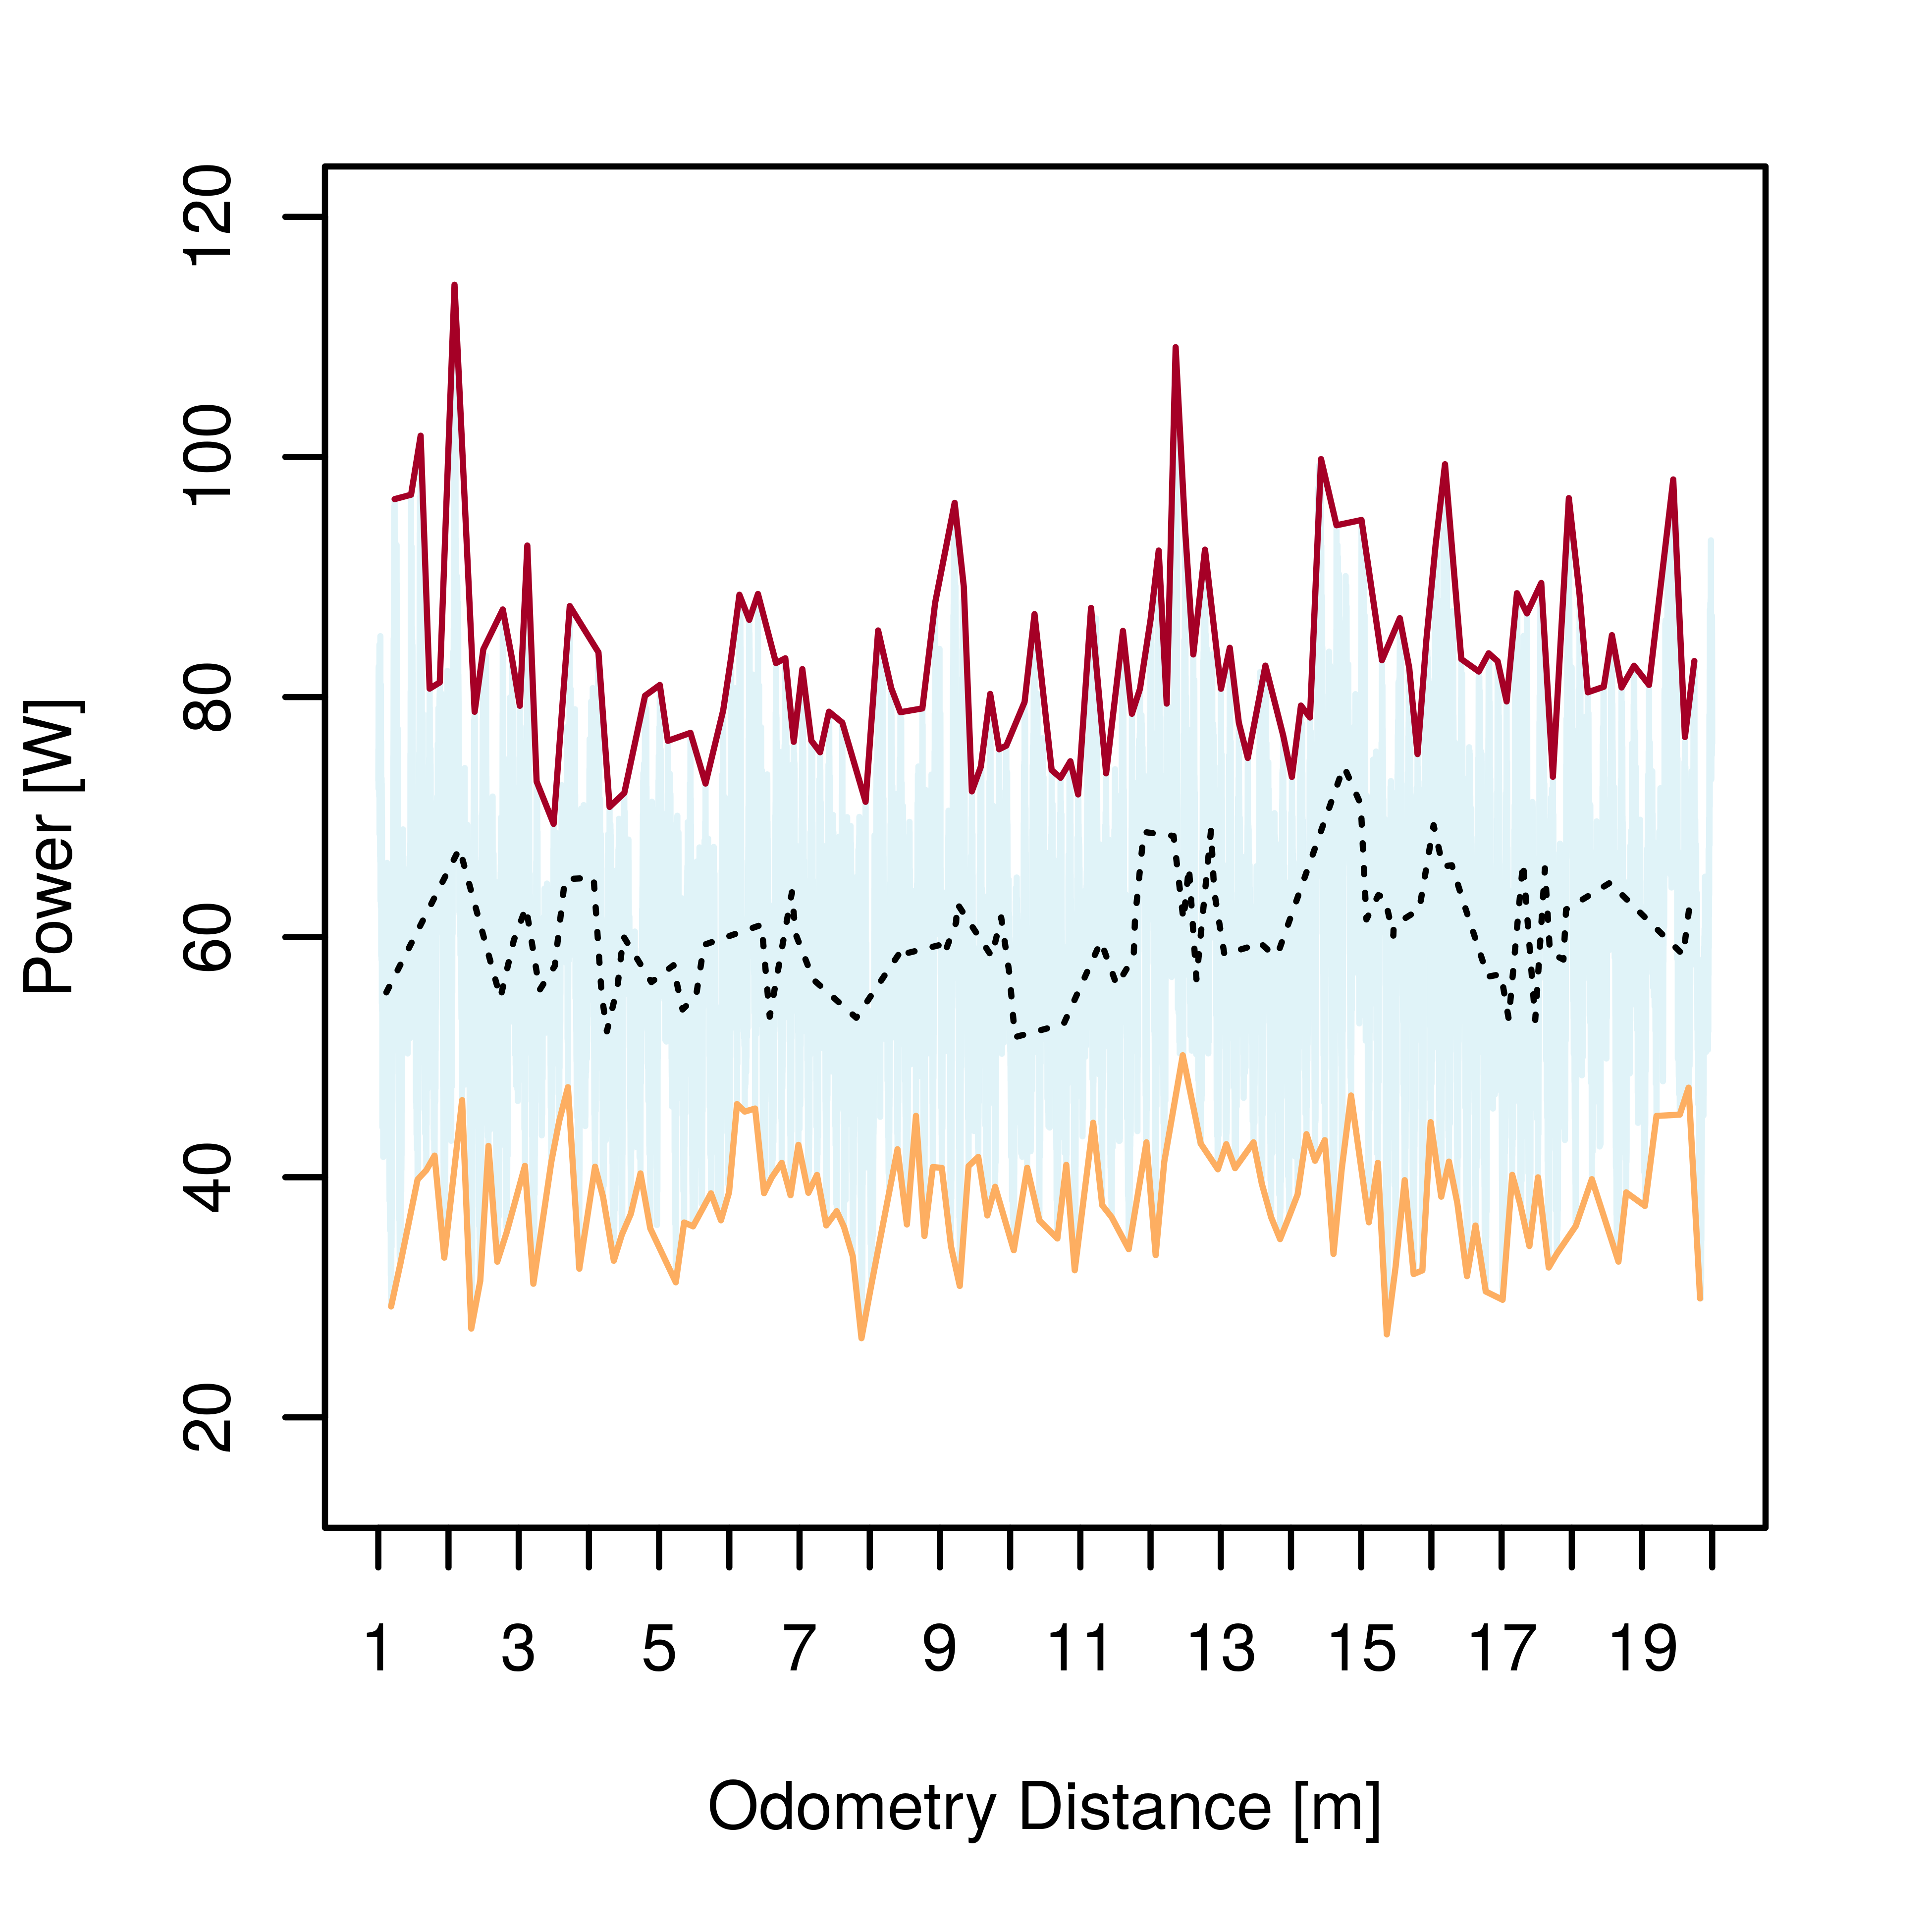
\includegraphics[height=\graphicsHeight]{sections/locomotion-power-draws/plots/locomotion-power-draw-on-flat-terrain-1.png}
        \subcaption{Run \#1}
        \label{fig:plot:sub:sherpatt-flat-terrain-power-draw-1}
    \end{subfigure}\hfill
    \begin{subfigure}[t]{\subfigureWidth}
        \centering
        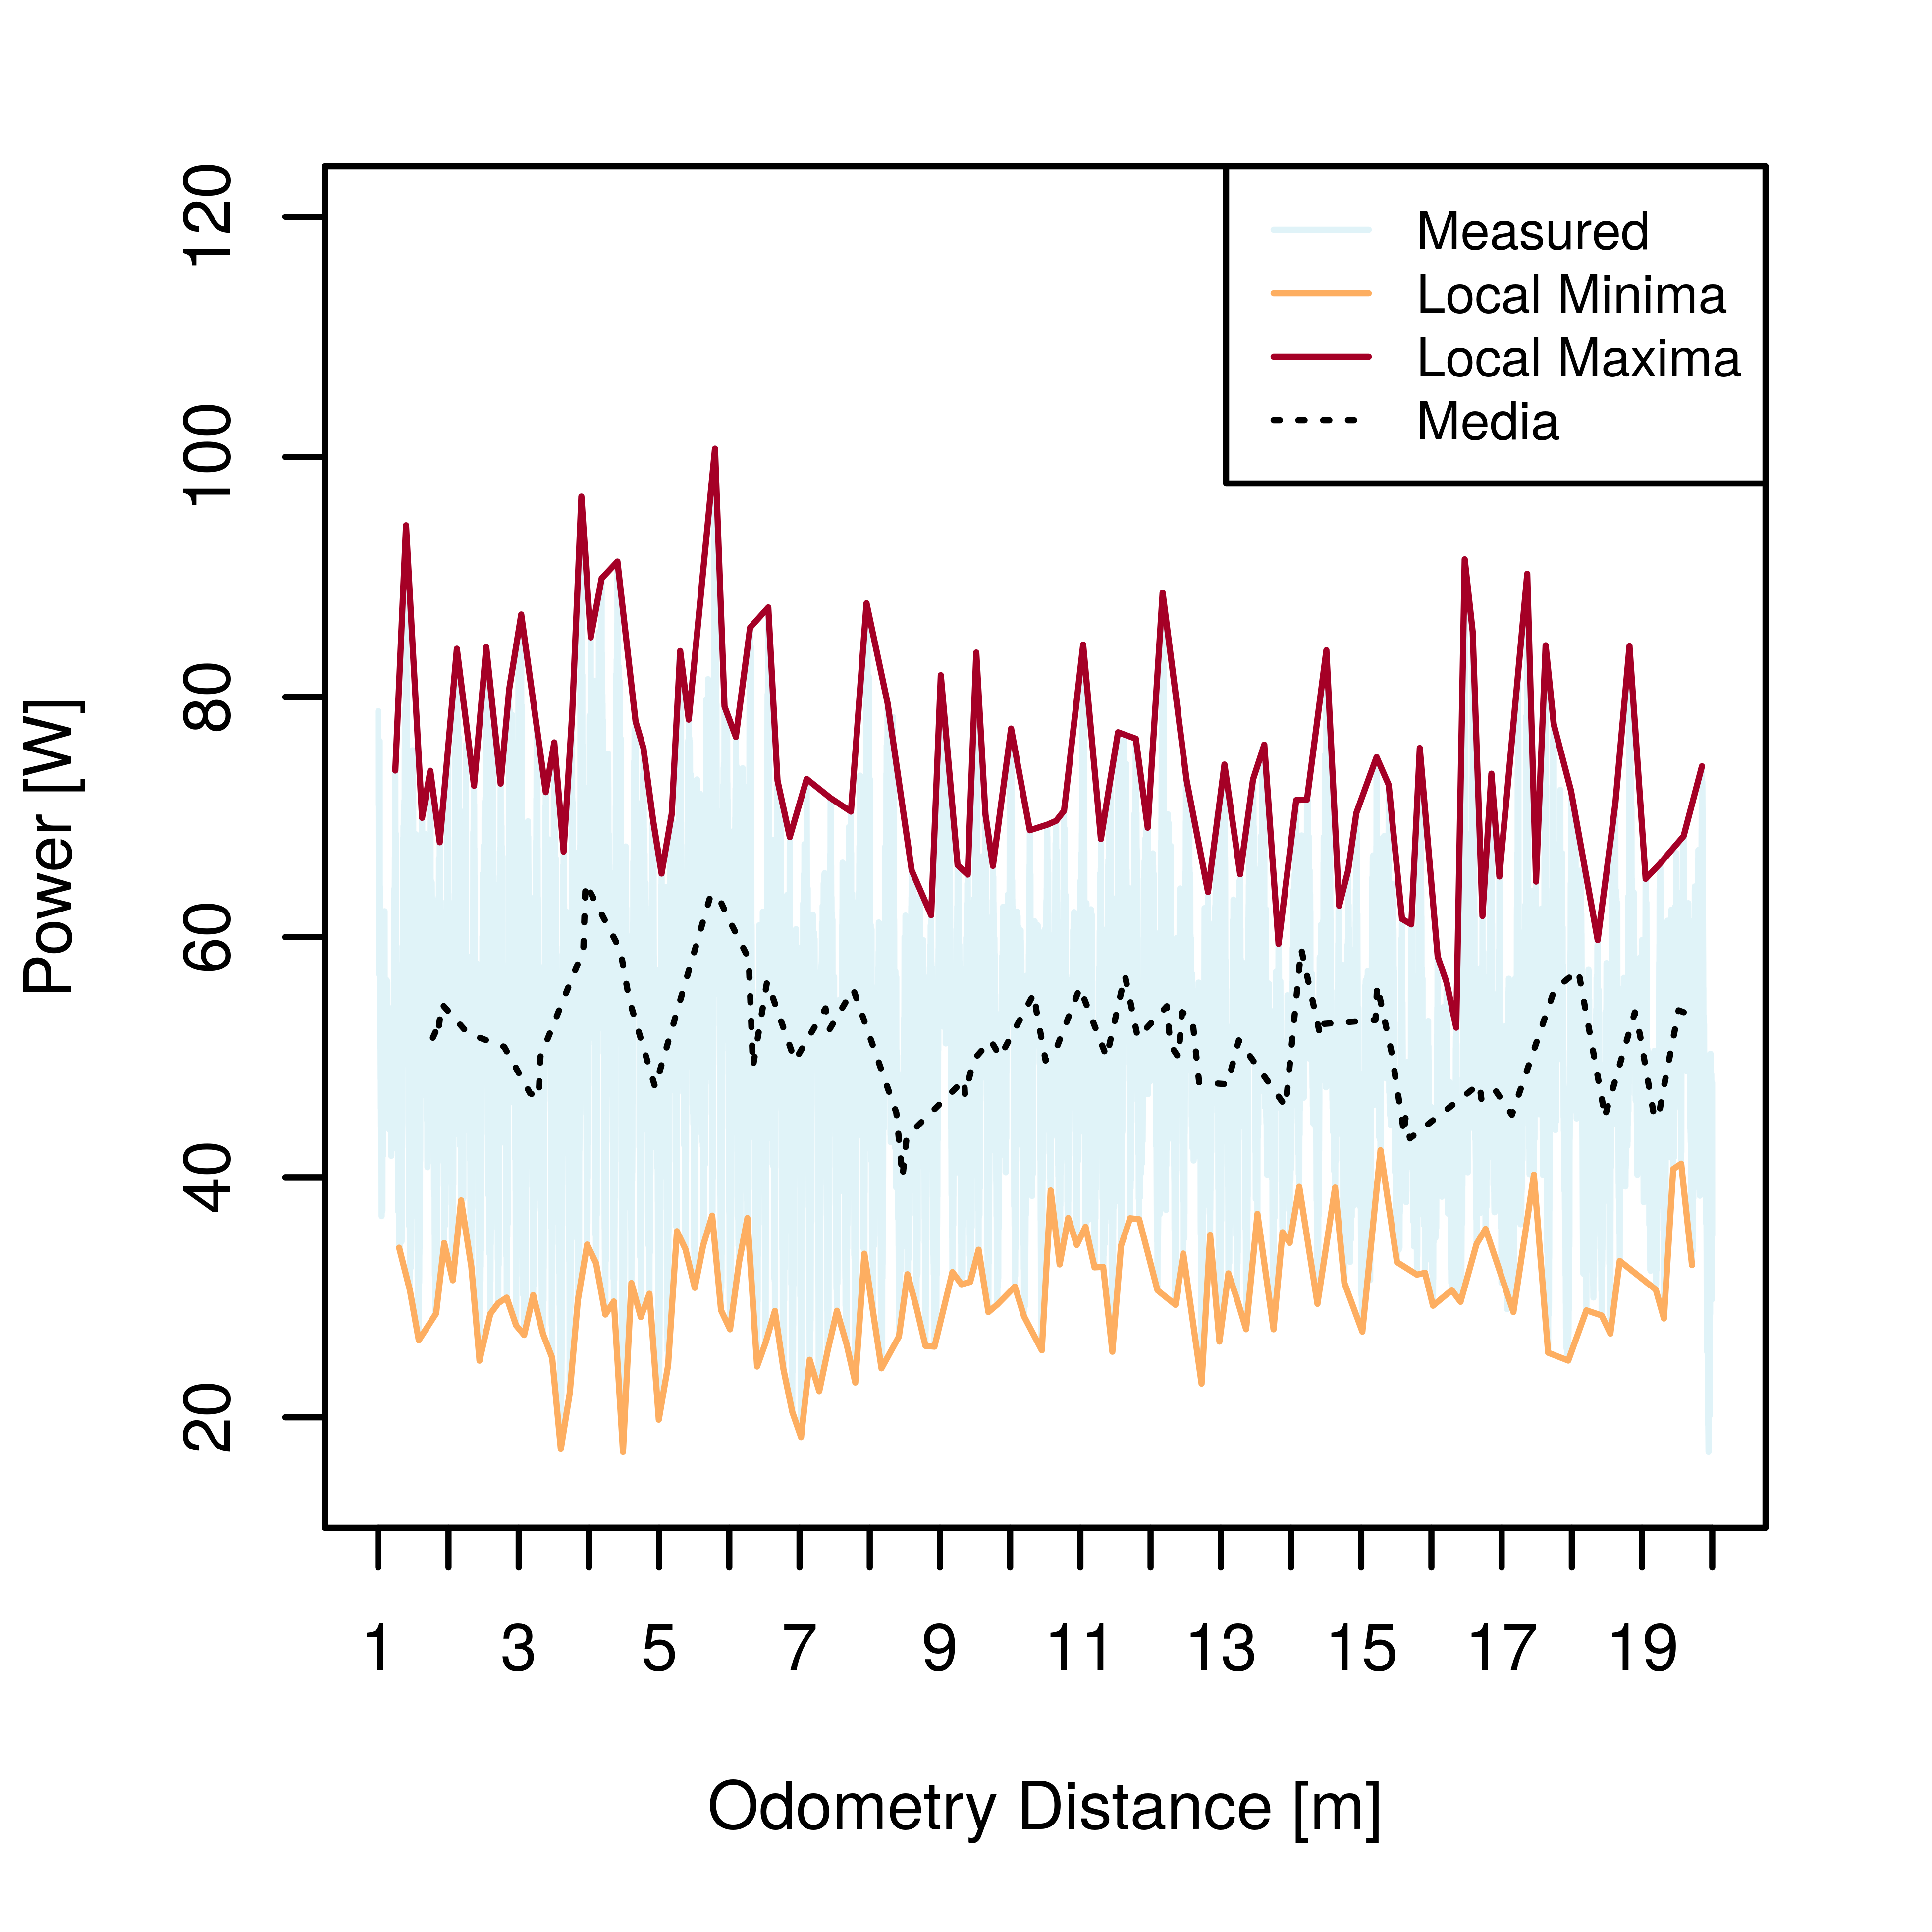
\includegraphics[height=\graphicsHeight]{sections/locomotion-power-draws/plots/locomotion-power-draw-on-flat-terrain-2.png}
  		\subcaption{Run \#2}
		\label{fig:plot:sub:sherpatt-flat-terrain-power-draw-2}
	\end{subfigure}\\[0.8ex]
    \caption[Propulsion power draw for a flat terrain traverse during SherpaTT Mars analogue field tests in Utah]
            {Propulsion power draw for a flat terrain traverse during SherpaTT Mars analogue field tests in Utah.}
    \label{fig:plot:sherpatt-flat-terrain-power-draw}
\vspace{-2ex}
\end{figure}


These measurements are summarised in Table \ref{tab:sherpatt-flat-terrain-global-minimum-maximum-and-medium-power-draws}. To eliminate power draw fluctuations from the analysis, only local media values were considered. Local media were selected rather than the worst-case local maxima on the basis of the assumptions made in Section \ref{sec:PropulsionPowerConstraints:Introduction}. For flat terrain traverses, a worst-case maximum power draw of \SI{74}{\watt} is observed for a mean of \SI{61}{\watt}.

\clearpage
\begin{table}[h]
\centering
\caption{Global minimum, maximum, and medium of traced local minima, maxima, and media for SherpaTT flat terrain propulsion power draw lines.}
\label{tab:sherpatt-flat-terrain-global-minimum-maximum-and-medium-power-draws}
\begin{tabular}{llccc}
\cline{3-5}
\multicolumn{2}{l|}{\multirow{2}{*}{}} & \multicolumn{3}{c|}{\textbf{Power Draw {[}W{]}}} \\ \cline{3-5}
\multicolumn{2}{l|}{} & \multicolumn{1}{c|}{\textbf{\begin{tabular}[c]{@{}c@{}}Global Minimum\end{tabular}}} & \multicolumn{1}{c|}{\textbf{\begin{tabular}[c]{@{}c@{}}Global Maximum\end{tabular}}} & \multicolumn{1}{c|}{\textbf{\begin{tabular}[c]{@{}c@{}}Global Media\end{tabular}}} \\ \hline
\multicolumn{1}{|c|}{\multirow{4}{*}{\textbf{Run \#1}}} & \multicolumn{1}{l|}{\textbf{Measured}} & \multicolumn{1}{c|}{27} & \multicolumn{1}{c|}{114} & \multicolumn{1}{c|}{60} \\ \cline{2-5}
\multicolumn{1}{|c|}{} & \multicolumn{1}{l|}{\textbf{Local Minima}} & \multicolumn{1}{c|}{27} & \multicolumn{1}{c|}{50} & \multicolumn{1}{c|}{38} \\ \cline{2-5}
\multicolumn{1}{|c|}{} & \multicolumn{1}{l|}{\textbf{Local Maxima}} & \multicolumn{1}{c|}{69} & \multicolumn{1}{c|}{114} & \multicolumn{1}{c|}{83} \\ \cline{2-5}
\multicolumn{1}{|c|}{} & \multicolumn{1}{l|}{\textbf{Local Media}} & \multicolumn{1}{c|}{52} & \multicolumn{1}{c|}{74} & \multicolumn{1}{c|}{61} \\ \hhline{|=|=|=|=|=|}
\multicolumn{1}{|l|}{\multirow{4}{*}{\textbf{Run \#2}}} & \multicolumn{1}{l|}{\textbf{Measured}} & \multicolumn{1}{c|}{17} & \multicolumn{1}{c|}{101} & \multicolumn{1}{c|}{51} \\ \cline{2-5}
\multicolumn{1}{|l|}{} & \multicolumn{1}{l|}{\textbf{Local Minima}} & \multicolumn{1}{c|}{17} & \multicolumn{1}{c|}{42} & \multicolumn{1}{c|}{30} \\ \cline{2-5}
\multicolumn{1}{|l|}{} & \multicolumn{1}{l|}{\textbf{Local Maxima}} & \multicolumn{1}{c|}{52} & \multicolumn{1}{c|}{101} & \multicolumn{1}{c|}{74} \\ \cline{2-5}
\multicolumn{1}{|l|}{} & \multicolumn{1}{l|}{\textbf{Local Media}} & \multicolumn{1}{c|}{40} & \multicolumn{1}{c|}{64} & \multicolumn{1}{c|}{52} \\ \hline
 &  & \multicolumn{1}{l}{} & \multicolumn{1}{l}{} & \multicolumn{1}{l}{} \\
 &  & \multicolumn{1}{l}{} & \multicolumn{1}{l}{} & \multicolumn{1}{l}{}
\end{tabular}
\end{table}


\subsection{Upslope Terrain Traverse}
\label{sec:PropulsionPowerConstraints:UpslopeTerrainTraverse}
Propulsion power draws on a steep uplsope were measured along an approximately \SI{16}{\meter} track and are shown Figure \ref{fig:plot:sub:sherpatt-disaggregated-upslope-terrain-power-draw-locomotion}. The drive and suspension power draw components are shown in Figures \ref{fig:plot:sub:sherpatt-disaggregated-upslope-terrain-power-draw-drive} and \ref{fig:plot:sub:sherpatt-disaggregated-upslope-terrain-power-draw-suspension}, respectively.

\begin{figure}[h]
\captionsetup[subfigure]{justification=centering}
\vspace{-2ex}
	\centering
    %% setup sizes
    \setlength{\subfigureWidth}{0.32\textwidth}
    \setlength{\graphicsHeight}{50mm}
    %% kill hyper-link highlighting
    \hypersetup{hidelinks=true}%
    %% the figures
	\begin{subfigure}[t]{\subfigureWidth}
        \centering
        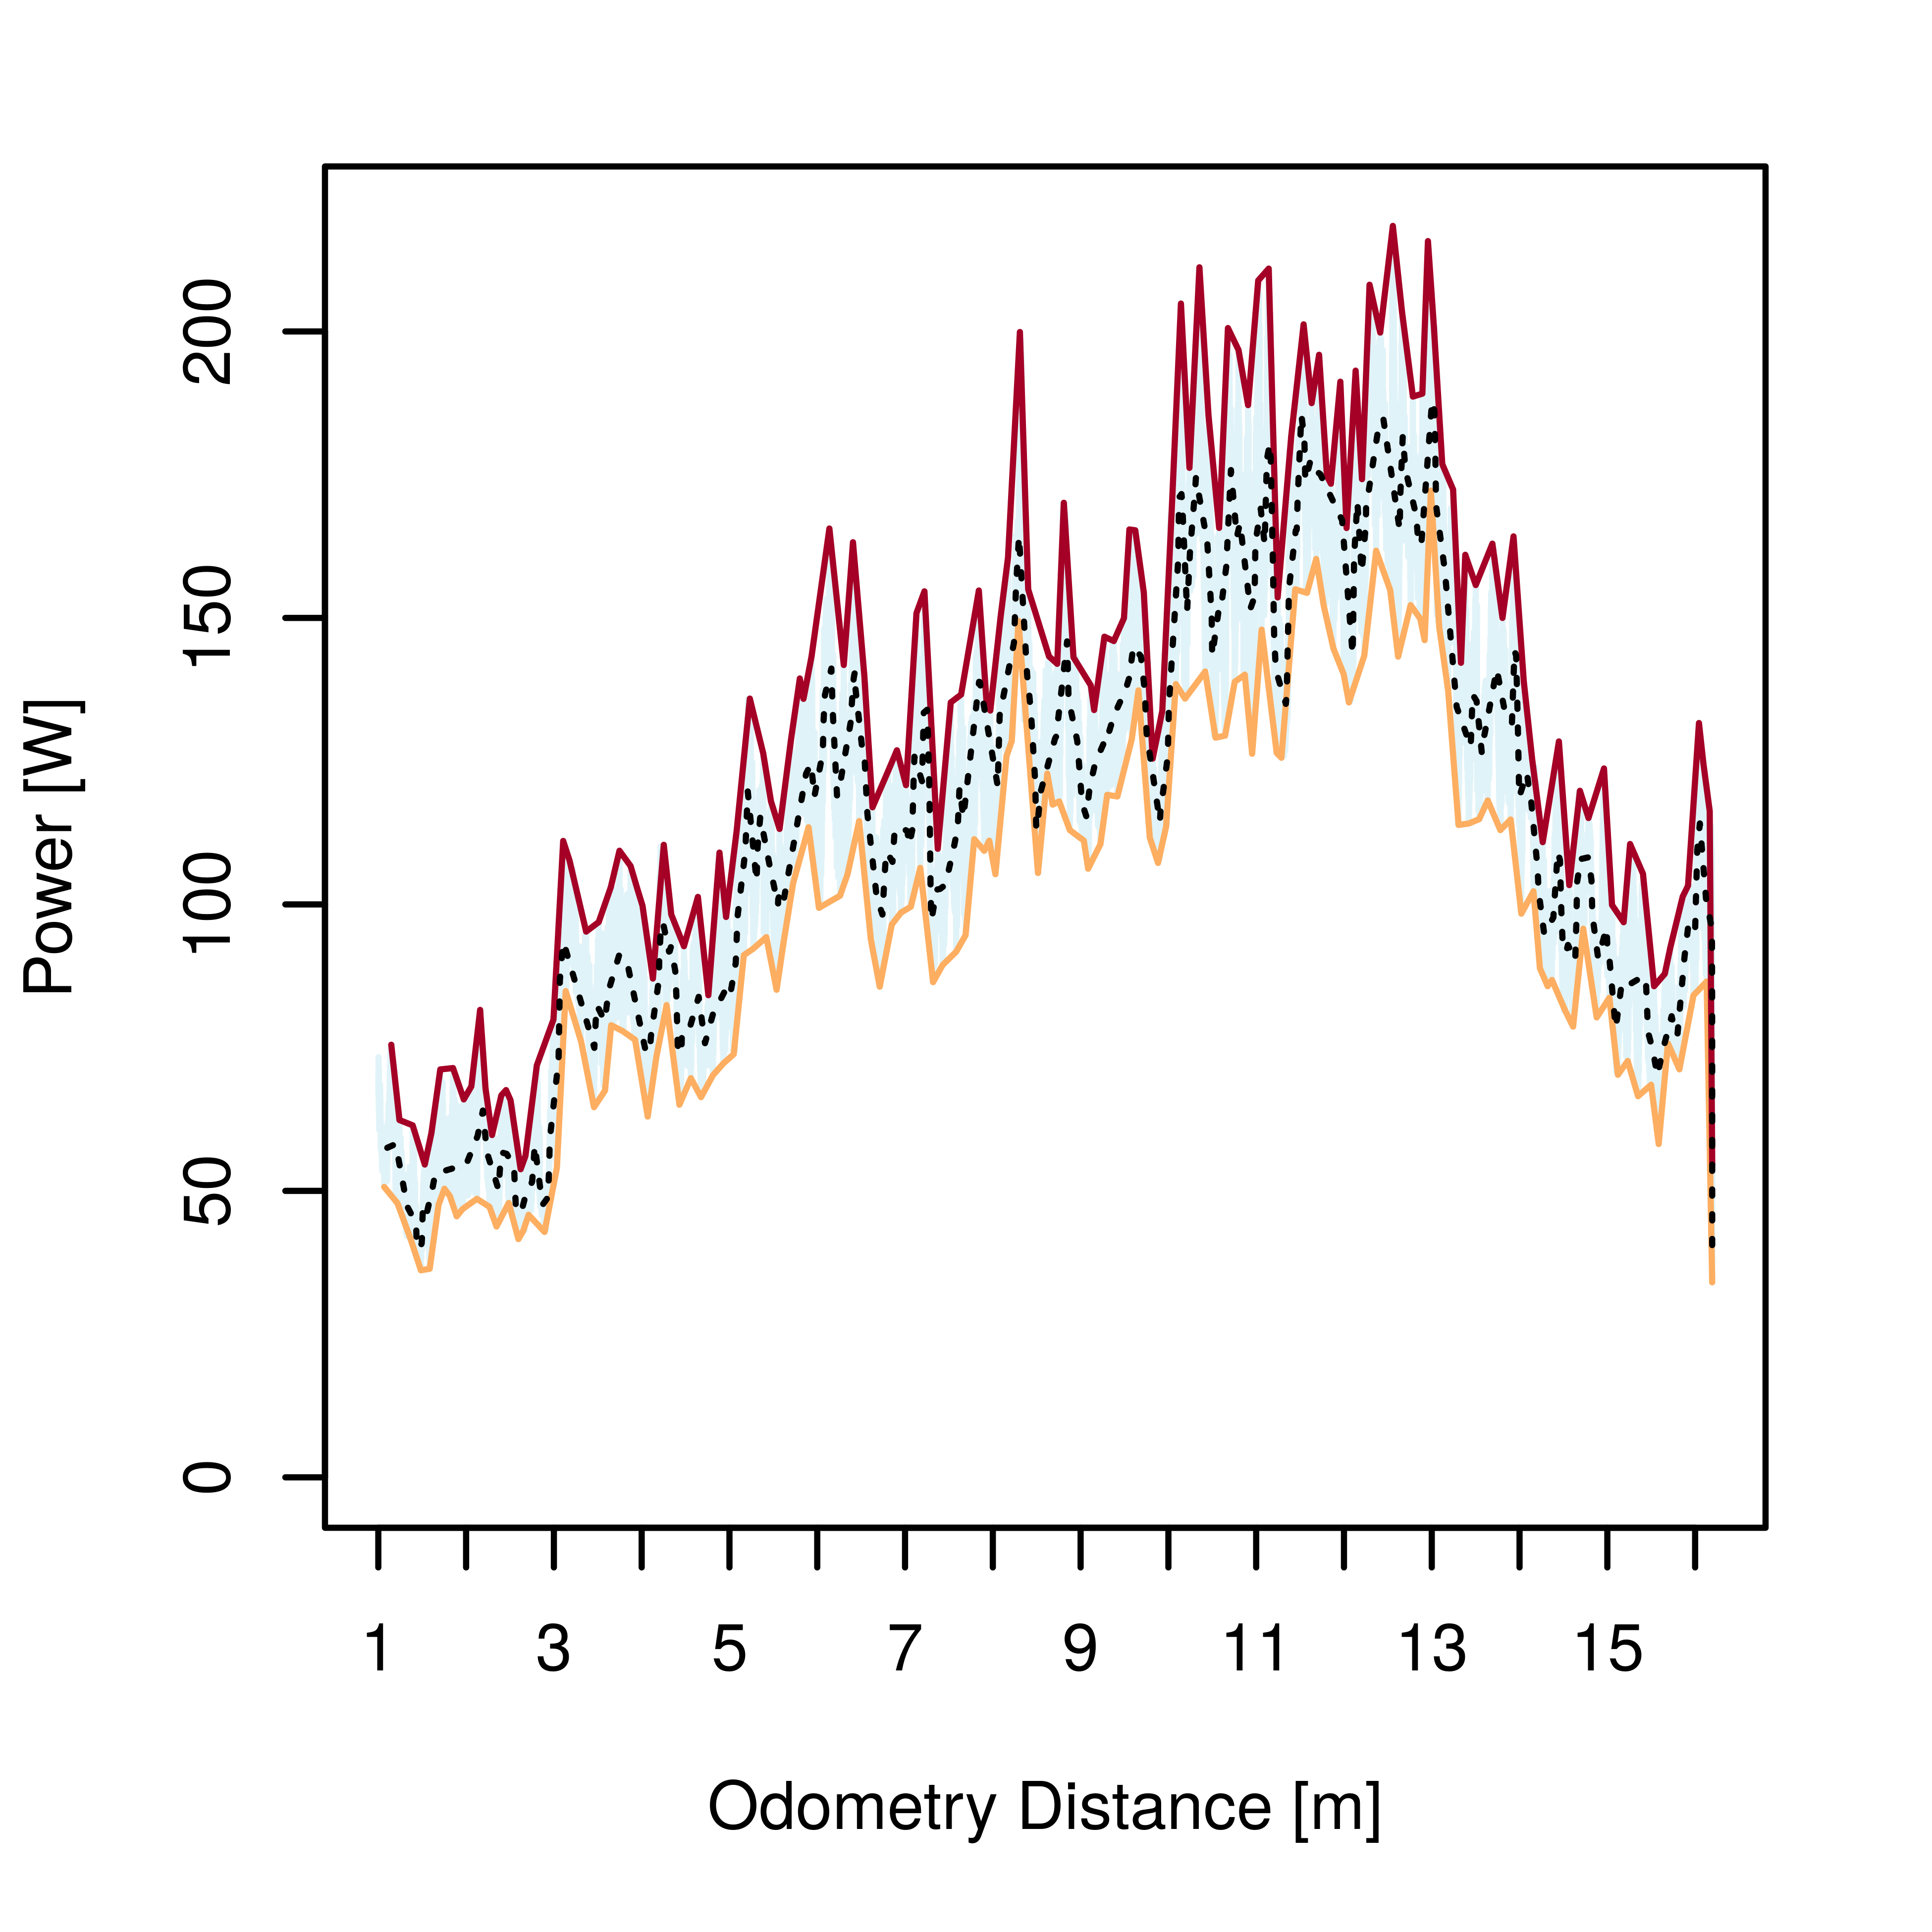
\includegraphics[height=\graphicsHeight]{sections/locomotion-power-draws/plots/locomotion-power-draw-on-upslope-terrain.png}
  		\subcaption{Propulsion}
		\label{fig:plot:sub:sherpatt-disaggregated-upslope-terrain-power-draw-locomotion}
	\end{subfigure}\hfill
	\begin{subfigure}[t]{\subfigureWidth}
        \centering
        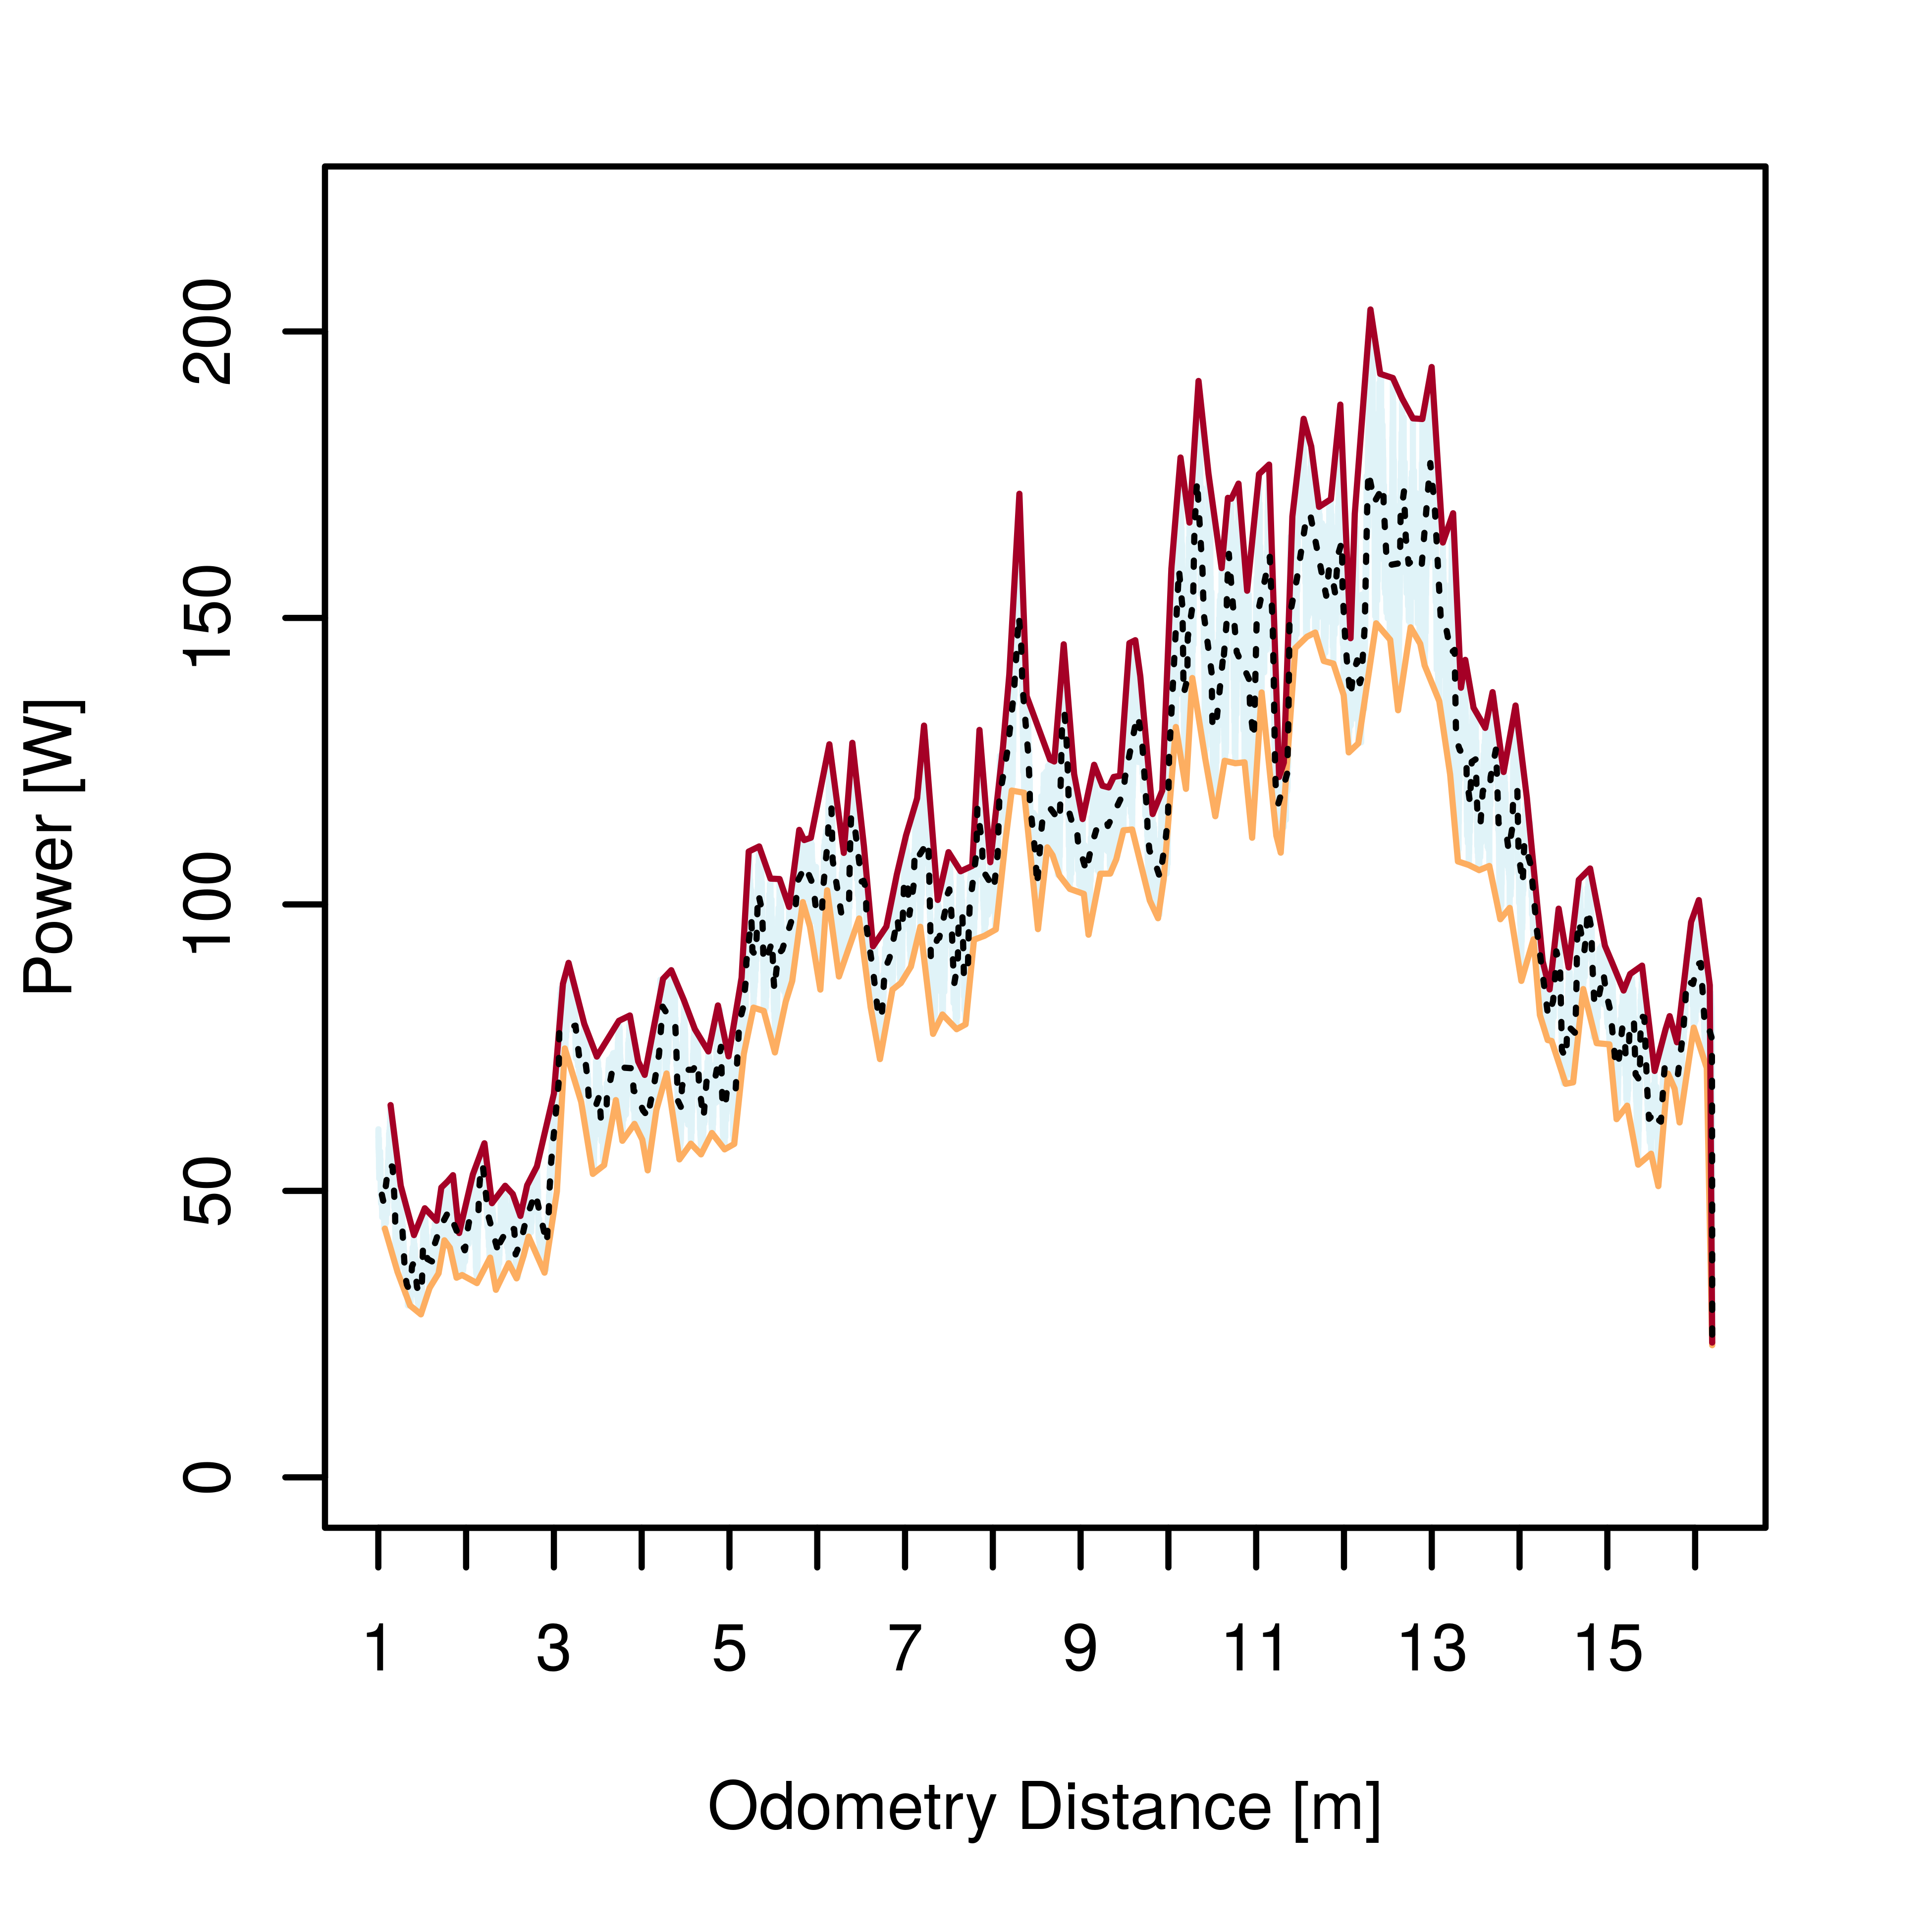
\includegraphics[height=\graphicsHeight]{sections/locomotion-power-draws/plots/drive-power-draw-on-upslope-terrain.png}
  		\subcaption{Drive}
		\label{fig:plot:sub:sherpatt-disaggregated-upslope-terrain-power-draw-drive}
	\end{subfigure}\hfill
    \begin{subfigure}[t]{\subfigureWidth}
        \centering
        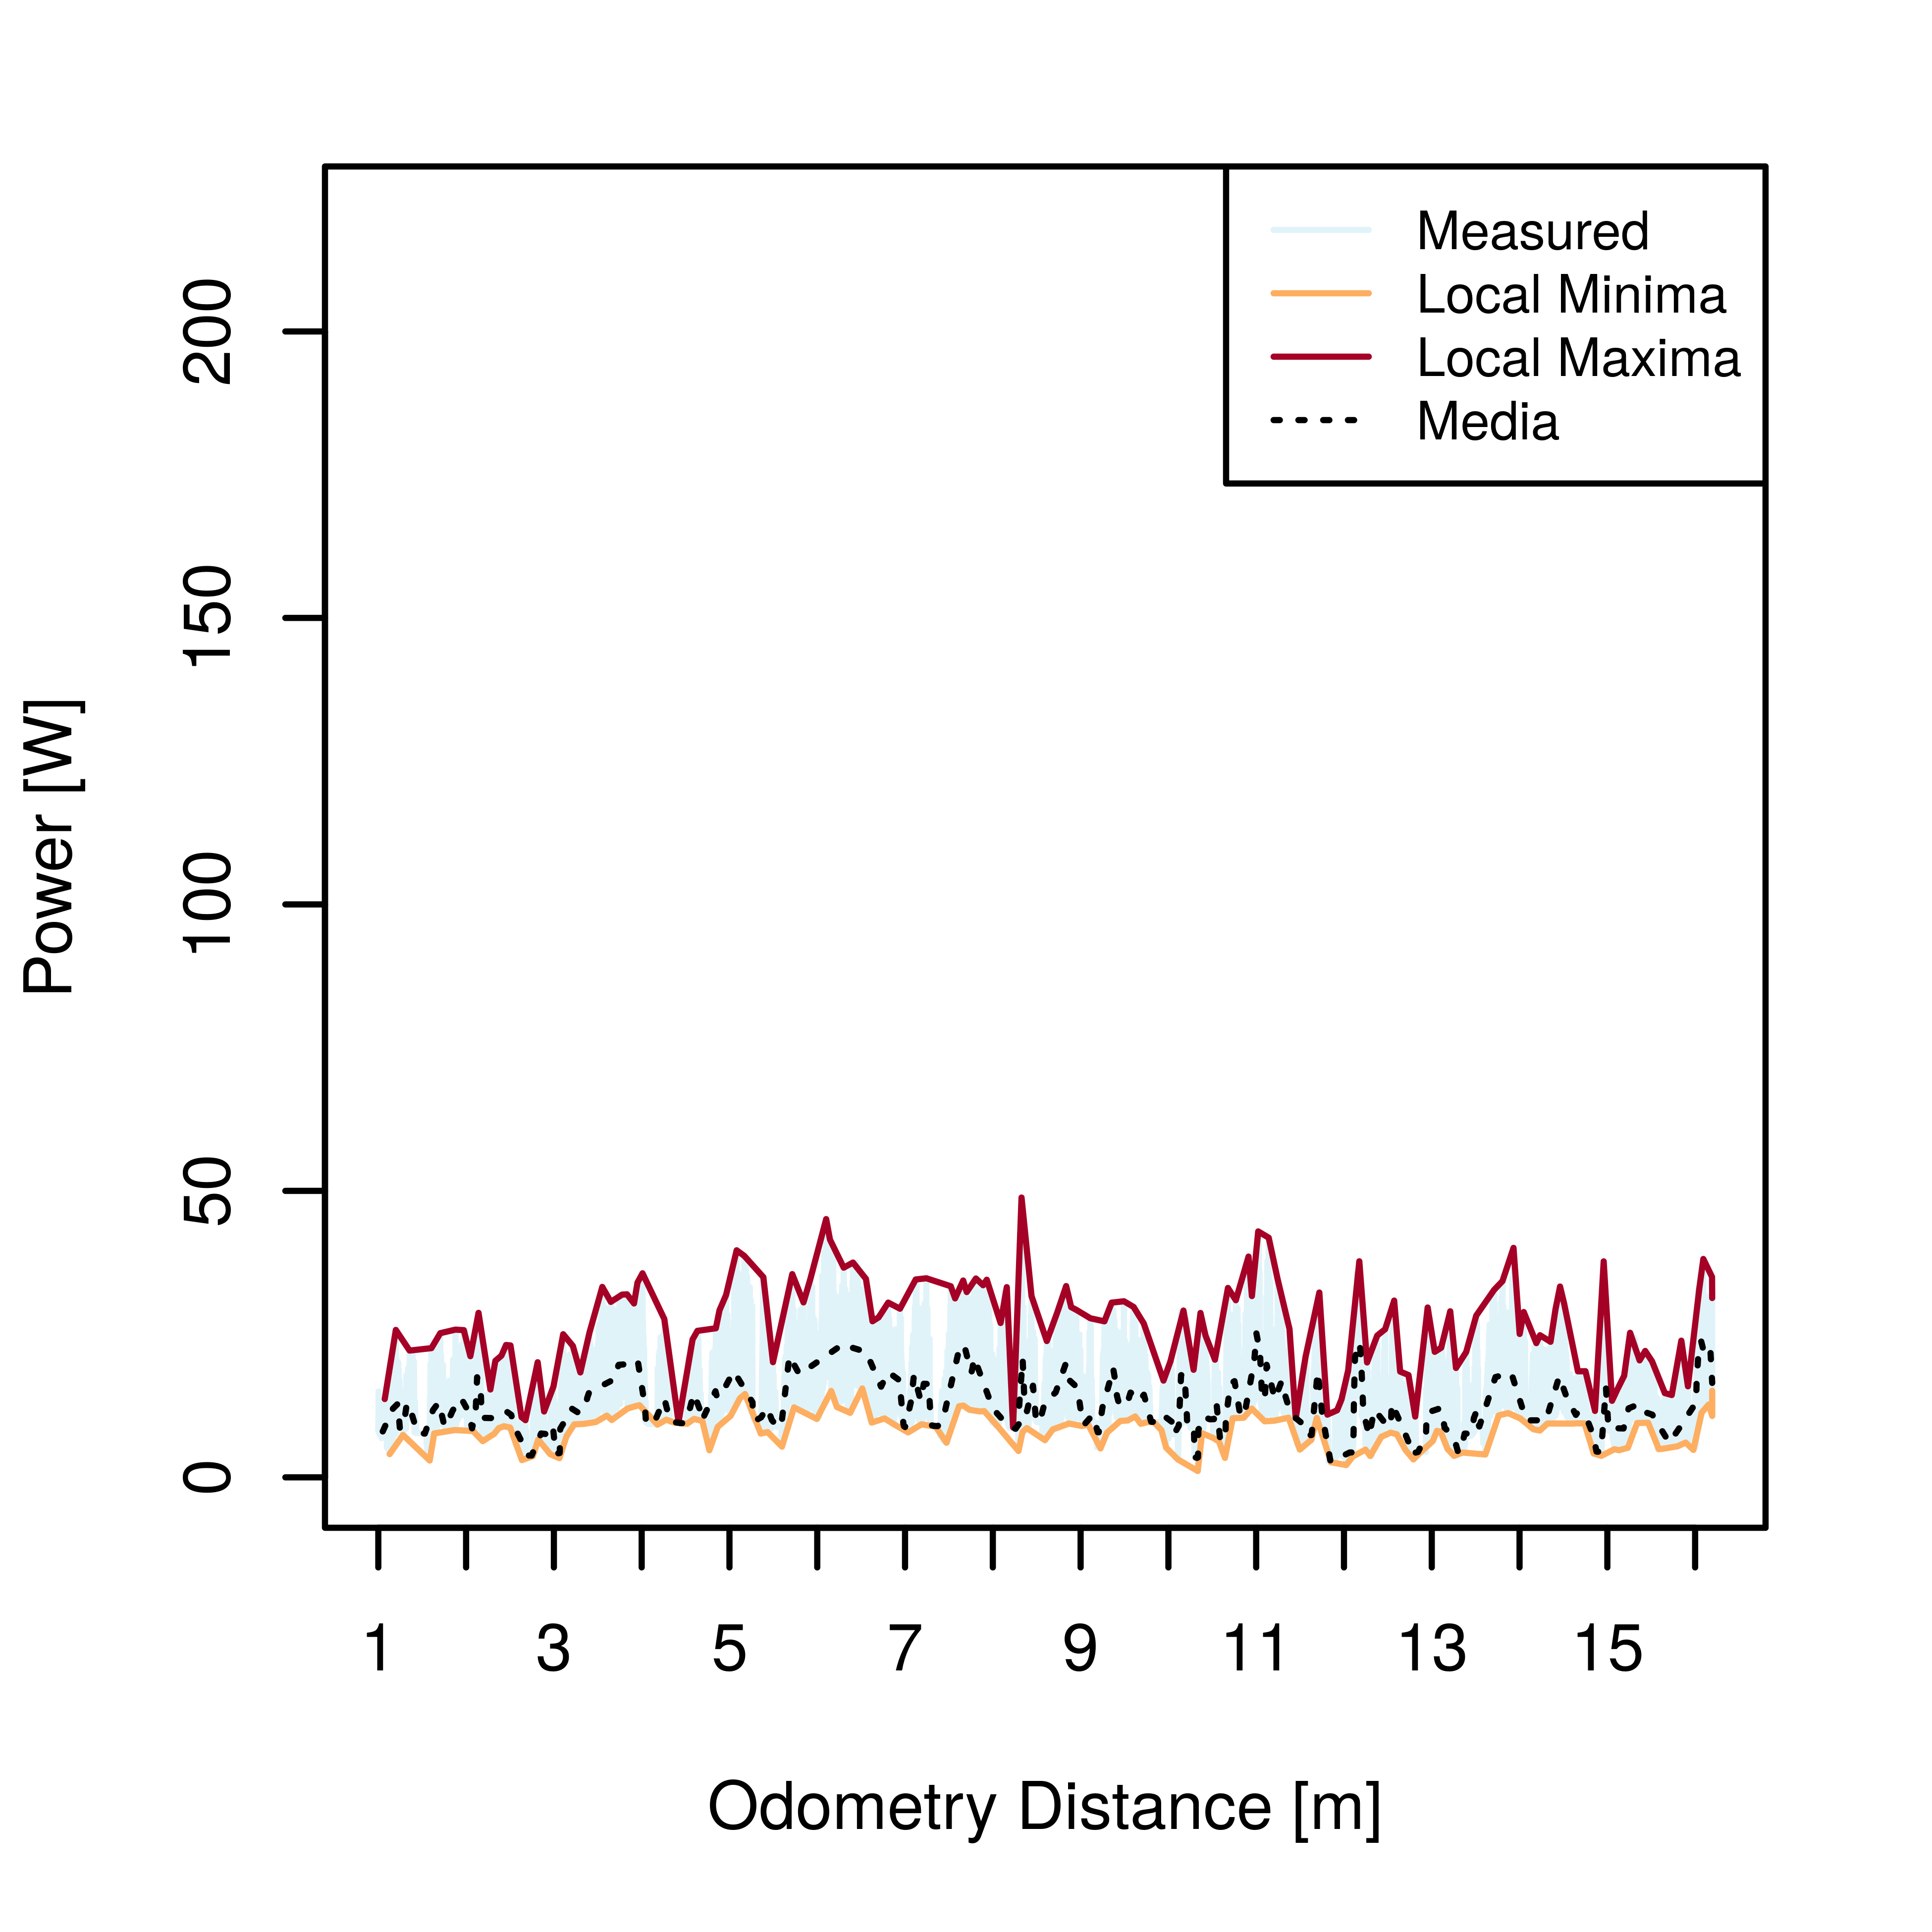
\includegraphics[height=\graphicsHeight]{sections/locomotion-power-draws/plots/suspension-power-draw-on-upslope-terrain.png}
  		\subcaption{Suspension}
		\label{fig:plot:sub:sherpatt-disaggregated-upslope-terrain-power-draw-suspension}
	\end{subfigure}\\[0.8ex]
    \caption[Disaggregated measurements of power draw for upslope terrain traverse during SherpaTT Mars analogue field tests in Utah]
            {Disaggregated measurements of power draw for upslope terrain traverse during SherpaTT Mars analogue field tests in Utah.}
    \label{fig:plot:sherpatt-disaggregated-upslope-terrain-power-draw}
\vspace{-2ex}
\end{figure}

An uplsope traverse has no discernable effect on the suspension power draw, however; there is a clear gradual increase in the drive power draw. The global maximum, minimum, and medium of the traced local minima, maxima, and media power draw lines are presented in Table \ref{tab:sherpatt-upslope-terrain-global-minimum-maximum-and-medium-power-draws}.

\clearpage
\begin{table}[h]
\centering
\caption{Global minimum, maximum, and medium of traced local minima, maxima, and media for SherpaTT upslope terrain traverse propulsion power draw lines.}
\label{tab:sherpatt-upslope-terrain-global-minimum-maximum-and-medium-power-draws}
\begin{tabular}{l|c|c|c|}
\cline{2-4}
\multicolumn{1}{c|}{\multirow{2}{*}{\textbf{}}} & \multicolumn{3}{c|}{\textbf{Power Draw {[}W{]}}} \\ \cline{2-4}
\multicolumn{1}{c|}{} & \textbf{\begin{tabular}[c]{@{}c@{}}Global Minimum\end{tabular}} & \textbf{\begin{tabular}[c]{@{}c@{}}Global Maximum\end{tabular}} & \textbf{\begin{tabular}[c]{@{}c@{}}Global Media\end{tabular}} \\ \hline
\multicolumn{1}{|l|}{\textbf{Measured}} & 34 & 218 & 114 \\ \hline
\multicolumn{1}{|l|}{\textbf{Local Minima}} & 34 & 172 & 98 \\ \hline
\multicolumn{1}{|l|}{\textbf{Local Maxima}} & 54 & 218 & 133 \\ \hline
\multicolumn{1}{|l|}{\textbf{Local Media}} & 40 & 188 & 18 \\ \hline
\end{tabular}
\end{table}


Figure \ref{fig:plot:sherpatt-upslope-terrain-power-draw} overlaps the propulsion local media power draws with the tackled slope angles. The steepest slope angle was \SI{28}{\degree} for an average of \SI{17.52}{\degree}. Slope angle increase are consistently followed by power draw spikes, i.e. at approximately 3, 4, 5, 6, 8, and 9 meters in the odometry measurements. Inversely, slope angle decreases were followed by power draws troughs at approximately 11, 13, 14, and 16 meters.

\begin{figure}[h]
  \centering
  \hypersetup{linkcolor=captionTextColor}
  \includegraphics[width=0.8\linewidth]{sections/locomotion-power-draws/plots/minima-locomotion-power-draws-on-upslope-terrain.png}\\
  \caption[Mean Propulsion power draw for an upslope terrain traverse during SherpaTT Utah field test campaign.]
          {Mean Propulsion power draw for an upslope terrain traverse during SherpaTT Utah field test campaign.}
  \label{fig:plot:sherpatt-upslope-terrain-power-draw}
\end{figure}

The power draws trough following the slope angle change from \SI{28}{\degree} to \SI{20}{\degree} at the \SI{11}{\meter} mark is subsequently followed by an unusual power draw increase and fluctuation. These measurements were discarded as they are outliers with respect to the power draw responses for the slope angle descreases that followed.

Table \ref{tab:sherpatt-upslope-terrain-local-media-measurement-summary} summarises the minimum, maximum, and mean local media propulsion power draws that were measured for different slope angles. Discarding the outlier measurements subsequent to the slope angle change from \SI{28}{\degree} to \SI{20}{\degree} at the \SI{11}{\meter} to \SI{13}{\meter} portion of the track, the maximum mean local media propulsion power draw is \SI{146}{\watt}.

\clearpage
\begin{table}[h]
\centering
\caption{SherpaTT mean propulsion power draw measurements for different slope sections}
\label{tab:sherpatt-upslope-terrain-local-media-measurement-summary}
\begin{tabular}{cc|c|c|c|}
\cline{3-5}
\multicolumn{1}{l}{} & \multicolumn{1}{l|}{} & \multicolumn{3}{c|}{\textbf{Power {[}W{]}}} \\ \hline
\multicolumn{1}{|l|}{\textbf{Distance {[}m{]}}} & \multicolumn{1}{l|}{\textbf{Slope Angle {[}deg{]}}} & \multicolumn{1}{l|}{\textbf{Minimum}} & \multicolumn{1}{l|}{\textbf{Maximum}} & \multicolumn{1}{l|}{\textbf{Mean}} \\ \hline
\multicolumn{1}{|c|}{\textbf{1 $<$ x $\leq$ 3}} & 10 & 40 & 64 & 51 \\ \hline
\multicolumn{1}{|c|}{\textbf{3 $<$ x $\leq$ 4}} & 11 & 73 & 93 & 85 \\ \hline
\multicolumn{1}{|c|}{\textbf{4 $<$ x $\leq$ 5}} & 15 & 74 & 87 & 83 \\ \hline
\multicolumn{1}{|c|}{\textbf{5 $<$ x $\leq$ 6}} & 16 & 85 & 125 & 107 \\ \hline
\multicolumn{1}{|c|}{\textbf{6 $<$ x $\leq$ 7}} & 28 & 98 & 141 & 123 \\ \hline
\multicolumn{1}{|c|}{\textbf{7 $<$ x $\leq$ 8}} & 22 & 97 & 139 & 116 \\ \hline
\multicolumn{1}{|c|}{\textbf{8 $<$ x $\leq$ 9}} & 25 & 113 & 164 & 133 \\ \hline
\multicolumn{1}{|c|}{\textbf{9 $<$ x $\leq$ 11}} & 28 & 114 & 176 & 146 \\ \hline
\multicolumn{1}{|c|}{\textbf{11 $<$ x $\leq$ 13}} & 20 & 135 & 188 & 167 \\ \hline
\multicolumn{1}{|c|}{\textbf{13 $<$ x $\leq$ 14}} & 15 & 119 & 123 & 145 \\ \hline
\multicolumn{1}{|c|}{\textbf{14 $<$ x $\leq$ 16}} & 10 & 70 & 186 & 94 \\ \hline
\end{tabular}
\end{table}


\section{Conclusion}
\label{sec:PropulsionPowerConstraints:Conclusion}
Based on data from the SherpaTT field campaign and the assumptions made in Section \ref{sec:PropulsionPowerConstraints:Introduction}, the following power subsystem requirements were proposed with respect to propulsion power draws:

\begin{itemize}
    \item The rover shall provide up to \SI{75}{\watt} in propulsion power for flat terrain traverses.
    \item The rover shall provide up to \SI{150}{\watt} in propulsion power for upslope terrain traverses of up to \SI{30}{\degree} inclination.
\end{itemize}


\clearpage
\section{Requirements and Design Drivers}
\label{sec:Design:RequirementsAndDesignDrivers}
\section{Introduction}
\label{sec:PropulsionPowerConstraints:Introduction}
SherpaTT's actively articulated suspension system consists of 4 wheeled-legs with a total of 20 motors. Each leg is equipped with 3 suspension motors and 2 drive motors. The suspension motors are responsible for Pan, \ac{IL}, and \ac{OL} revolute joint rotations whereas the drive motors are responsible for \ac{WS} and \ac{WD}. The distribution of these motors across each leg are shown in Figure \ref{fig:sherpatt-actively-articulated-suspension-system}. Propulsion power draw refers to the summation of suspension and drive motor power draws. These power draws have been studied in detail for SherpaTT during a Mars analogue field campaign in Utah \citeother{Cordes2018}.

\begin{figure}[h]
  \centering
  \hypersetup{linkcolor=captionTextColor}
  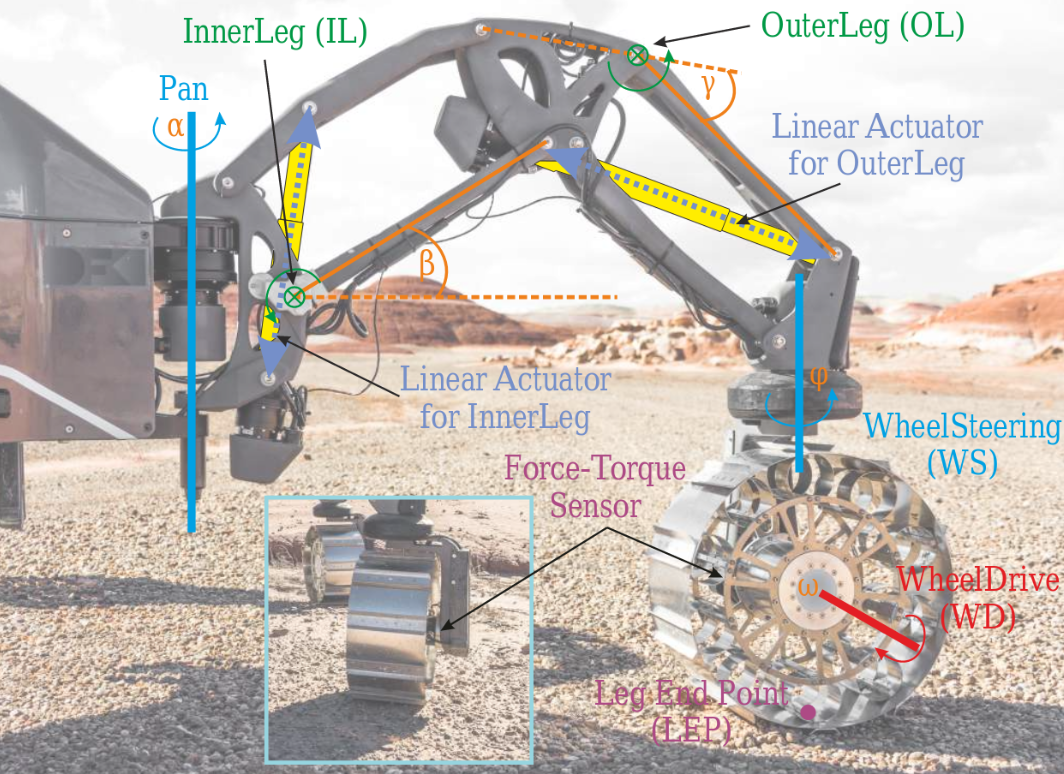
\includegraphics[width=0.8\linewidth]{sections/locomotion-power-draws/images/sherpatt-actively-articulated-suspension-sytem.png}\\
  \caption[SherpaTT actively articulated suspension system]
          {SherpaTT actively articulated suspension system.}
  \label{fig:sherpatt-actively-articulated-suspension-system}
\end{figure}

 This section restricts power draw analysis to establishing propulsion power constraints for the study of SherpaTT Mars mission scenarios. Lack of motor optimisation as well as lower gravity and pressure on Mars permit the assumption that, given similar topology traversals, measured propulsion power draws are greater than those that would be observed on a Martian environment. This assumption is further supported when considering that SherpaTT's velocities during power draw measurements were much greater than what has been achieved on present and past Mars rover missions.


\section{Power Draw}
\label{sec:PropulsionPowerConstraints:PowerDraw}
Available datasets from the Mars analogue field test campaign cover 2 flat surface runs and 3 steep upslope terrain runs. From the 2 upslope runs, the dataset with the worst-case maximum and mean propulsion power draw was used as the worst-case scenario. Hereafter, all mention of SherpaTT power draws will reference measurements included in these datasets. Measured power draws fluctuate due to slips, skids, noise, and other unknown imperfections. To ease readability, local minima, maxima, and media lines have been traced for all power plot figures.


\subsection{Flat Terrain Traverse}
\label{sec:PropulsionPowerConstraints:FlatTerrainTraverse}
\ac{MER} and \ac{MSL} rovers are each equipped with a total of 10 propulsion motors to drive their Rocker-Bogie passive suspension system: 6 to rotate the wheels and 4 to steer them \citeother{Novak2005} \citeother{Lakdawalla2018}. The \ac{MER} rovers needed approximately \SI{100}{\watt} to drive \citeother{MERRoverEnergy}. Propulsion power draws measured for SherpaTT on flat surface runs are shown in Figure \ref{fig:plot:sherpatt-flat-terrain-power-draw}.

\begin{figure}[h]
\captionsetup[subfigure]{justification=centering}
\vspace{-2ex}
	\centering
    %% setup sizes
    \setlength{\subfigureWidth}{0.50\textwidth}
    \setlength{\graphicsHeight}{80mm}
    %% kill hyper-link highlighting
    \hypersetup{hidelinks=true}%
    %% the figures
    \begin{subfigure}[t]{\subfigureWidth}
        \centering
        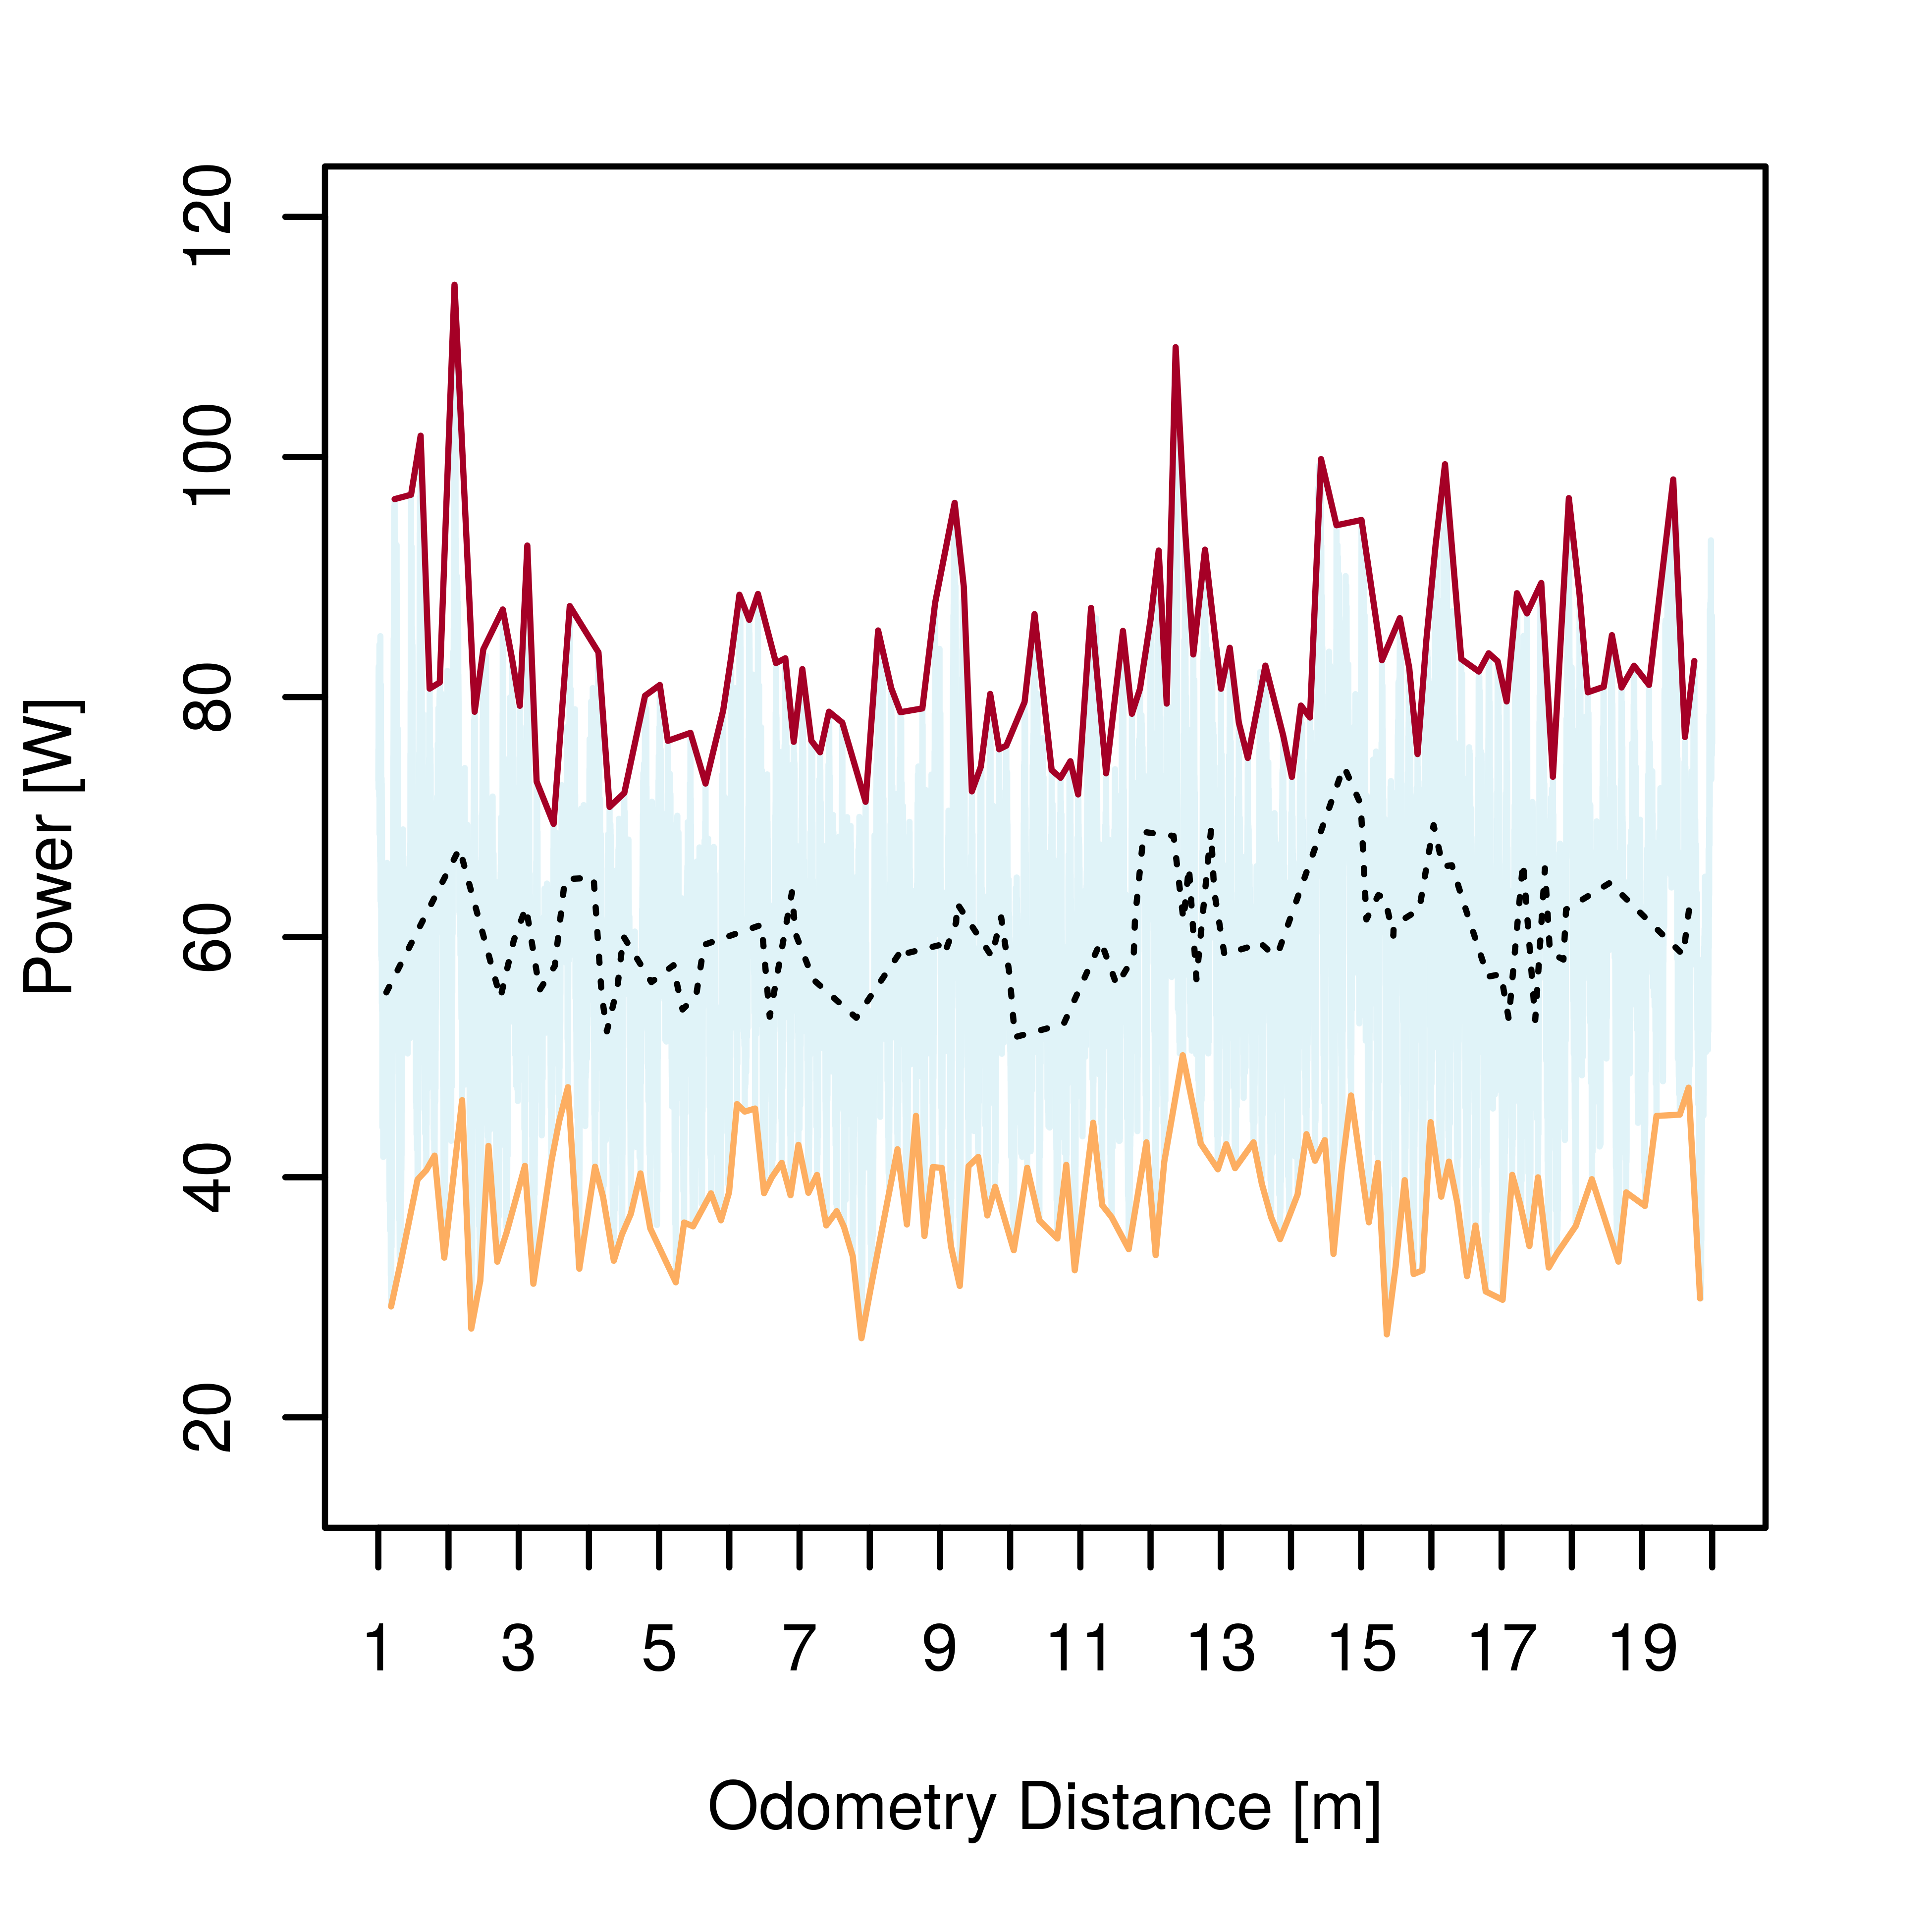
\includegraphics[height=\graphicsHeight]{sections/locomotion-power-draws/plots/locomotion-power-draw-on-flat-terrain-1.png}
        \subcaption{Run \#1}
        \label{fig:plot:sub:sherpatt-flat-terrain-power-draw-1}
    \end{subfigure}\hfill
    \begin{subfigure}[t]{\subfigureWidth}
        \centering
        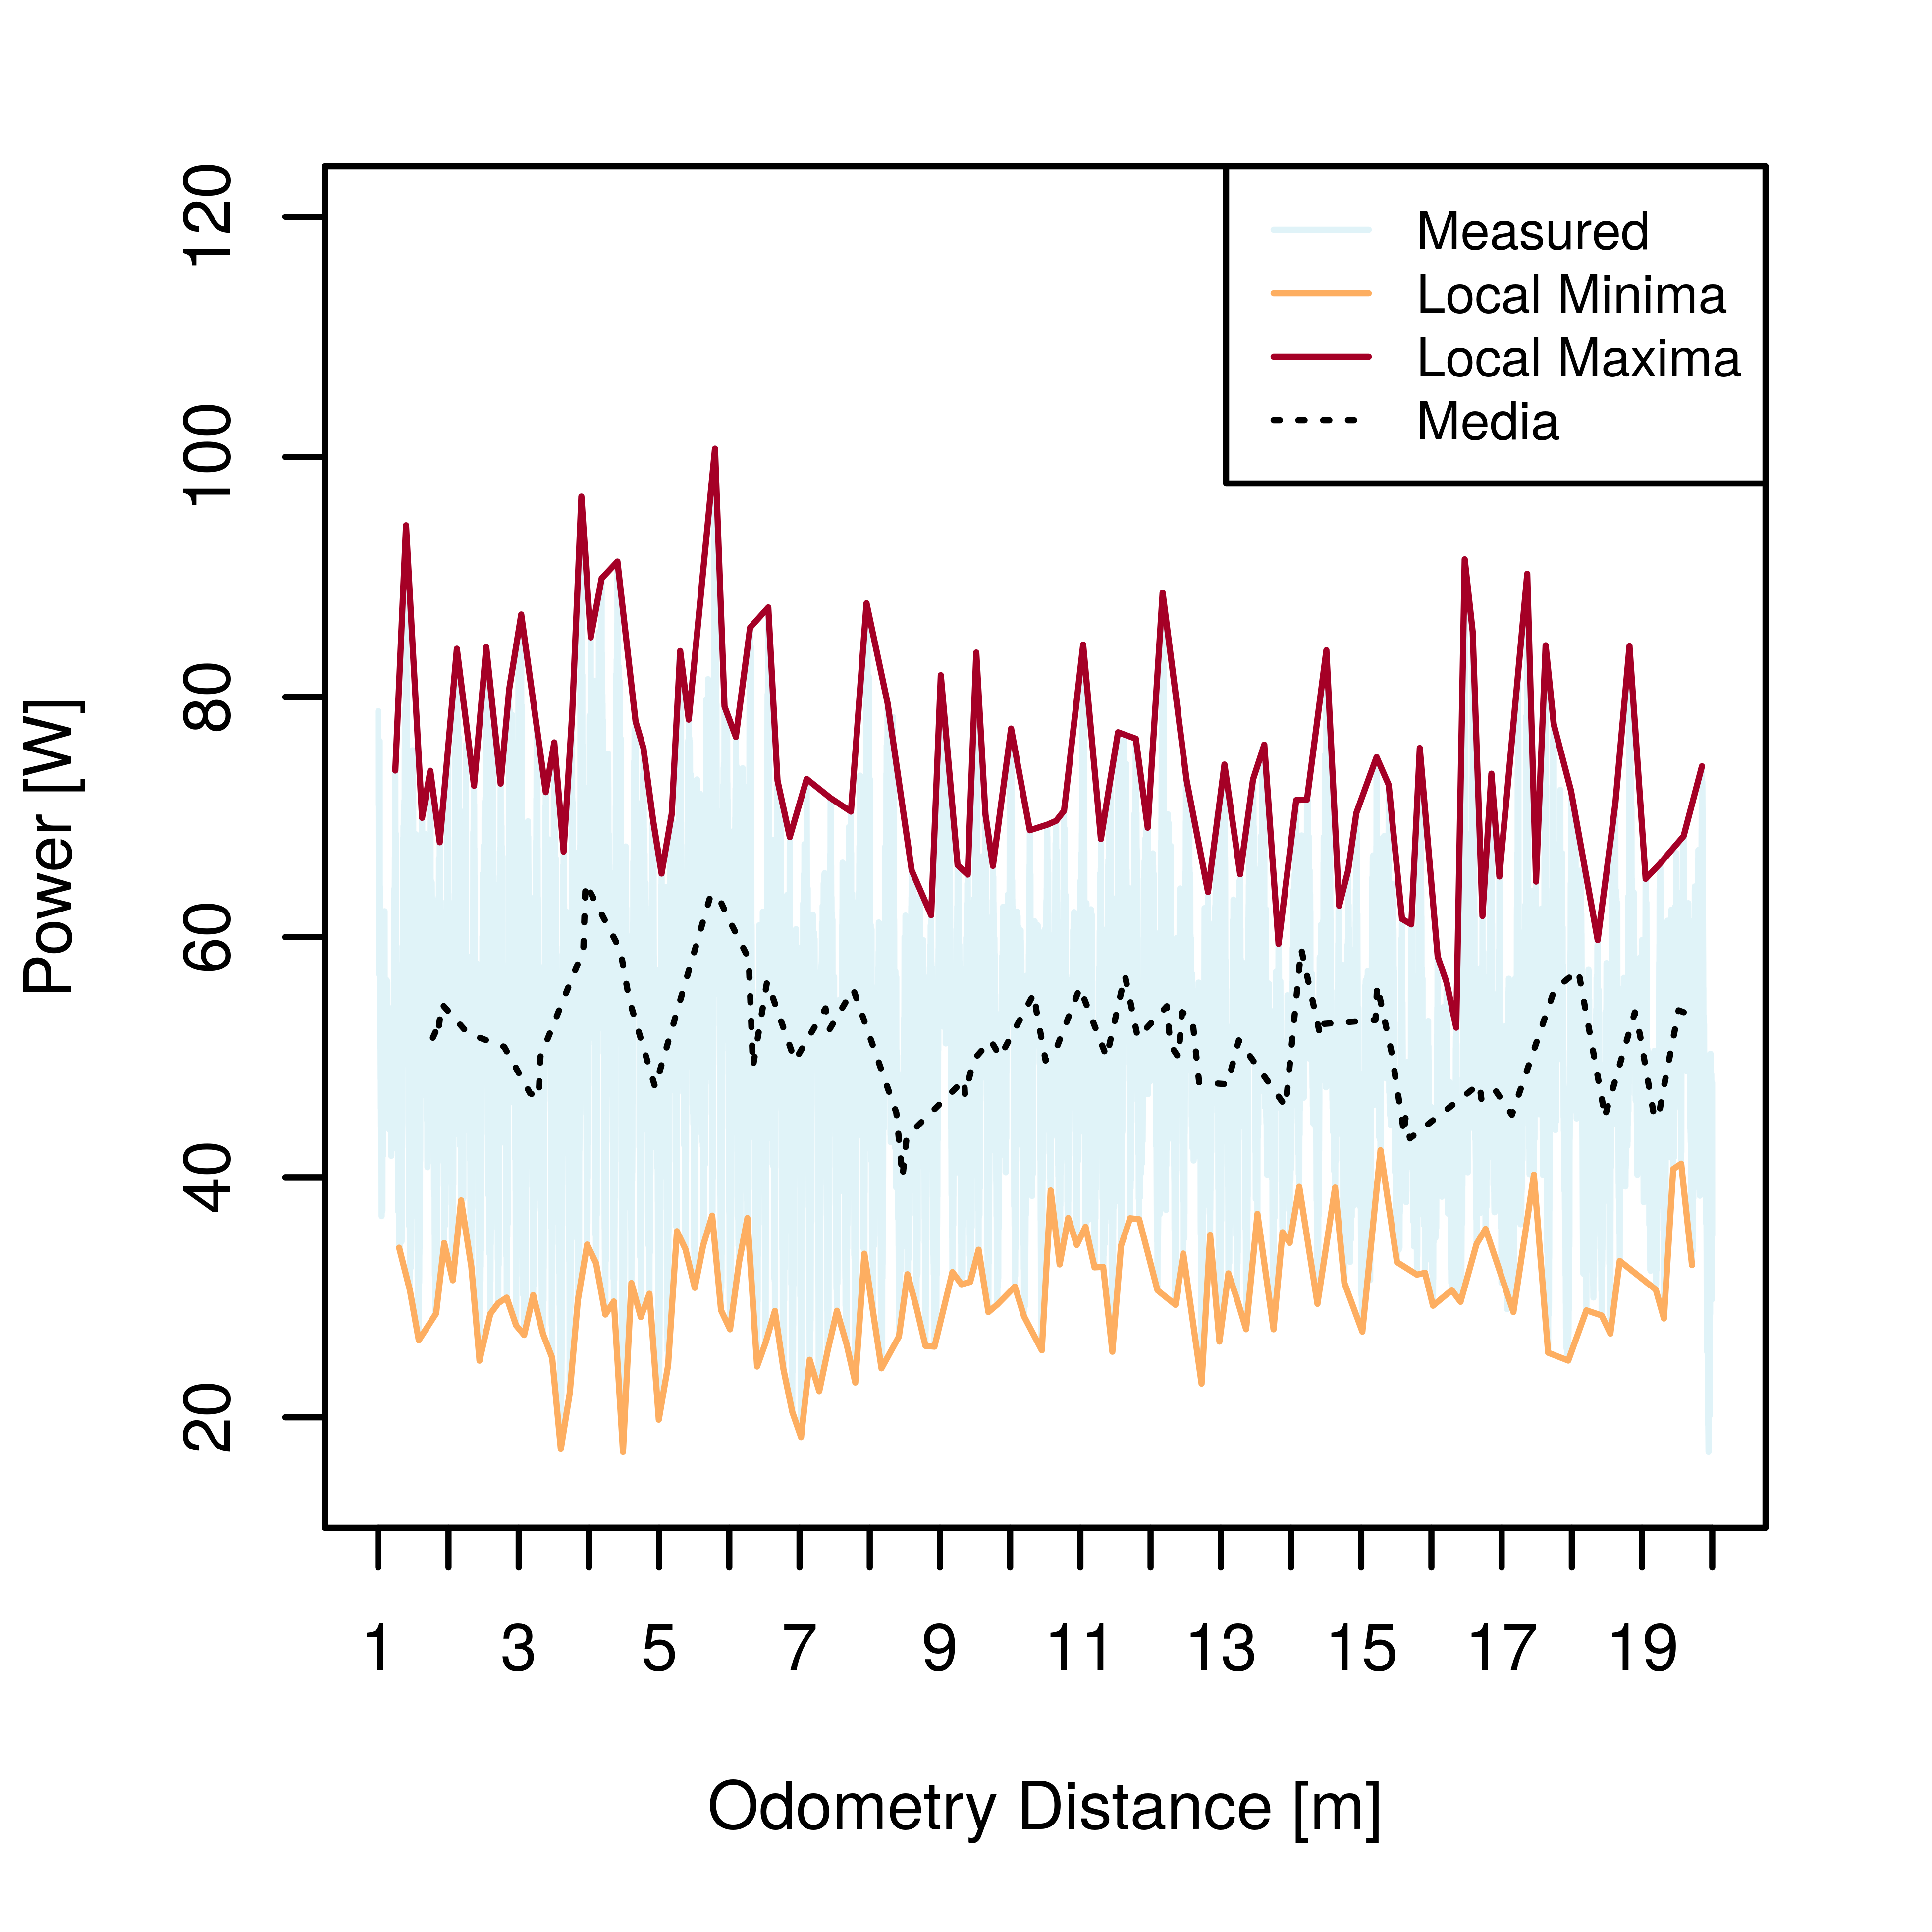
\includegraphics[height=\graphicsHeight]{sections/locomotion-power-draws/plots/locomotion-power-draw-on-flat-terrain-2.png}
  		\subcaption{Run \#2}
		\label{fig:plot:sub:sherpatt-flat-terrain-power-draw-2}
	\end{subfigure}\\[0.8ex]
    \caption[Propulsion power draw for a flat terrain traverse during SherpaTT Mars analogue field tests in Utah]
            {Propulsion power draw for a flat terrain traverse during SherpaTT Mars analogue field tests in Utah.}
    \label{fig:plot:sherpatt-flat-terrain-power-draw}
\vspace{-2ex}
\end{figure}


These measurements are summarised in Table \ref{tab:sherpatt-flat-terrain-global-minimum-maximum-and-medium-power-draws}. To eliminate power draw fluctuations from the analysis, only local media values were considered. Local media were selected rather than the worst-case local maxima on the basis of the assumptions made in Section \ref{sec:PropulsionPowerConstraints:Introduction}. For flat terrain traverses, a worst-case maximum power draw of \SI{74}{\watt} is observed for a mean of \SI{61}{\watt}.

\clearpage
\begin{table}[h]
\centering
\caption{Global minimum, maximum, and medium of traced local minima, maxima, and media for SherpaTT flat terrain propulsion power draw lines.}
\label{tab:sherpatt-flat-terrain-global-minimum-maximum-and-medium-power-draws}
\begin{tabular}{llccc}
\cline{3-5}
\multicolumn{2}{l|}{\multirow{2}{*}{}} & \multicolumn{3}{c|}{\textbf{Power Draw {[}W{]}}} \\ \cline{3-5}
\multicolumn{2}{l|}{} & \multicolumn{1}{c|}{\textbf{\begin{tabular}[c]{@{}c@{}}Global Minimum\end{tabular}}} & \multicolumn{1}{c|}{\textbf{\begin{tabular}[c]{@{}c@{}}Global Maximum\end{tabular}}} & \multicolumn{1}{c|}{\textbf{\begin{tabular}[c]{@{}c@{}}Global Media\end{tabular}}} \\ \hline
\multicolumn{1}{|c|}{\multirow{4}{*}{\textbf{Run \#1}}} & \multicolumn{1}{l|}{\textbf{Measured}} & \multicolumn{1}{c|}{27} & \multicolumn{1}{c|}{114} & \multicolumn{1}{c|}{60} \\ \cline{2-5}
\multicolumn{1}{|c|}{} & \multicolumn{1}{l|}{\textbf{Local Minima}} & \multicolumn{1}{c|}{27} & \multicolumn{1}{c|}{50} & \multicolumn{1}{c|}{38} \\ \cline{2-5}
\multicolumn{1}{|c|}{} & \multicolumn{1}{l|}{\textbf{Local Maxima}} & \multicolumn{1}{c|}{69} & \multicolumn{1}{c|}{114} & \multicolumn{1}{c|}{83} \\ \cline{2-5}
\multicolumn{1}{|c|}{} & \multicolumn{1}{l|}{\textbf{Local Media}} & \multicolumn{1}{c|}{52} & \multicolumn{1}{c|}{74} & \multicolumn{1}{c|}{61} \\ \hhline{|=|=|=|=|=|}
\multicolumn{1}{|l|}{\multirow{4}{*}{\textbf{Run \#2}}} & \multicolumn{1}{l|}{\textbf{Measured}} & \multicolumn{1}{c|}{17} & \multicolumn{1}{c|}{101} & \multicolumn{1}{c|}{51} \\ \cline{2-5}
\multicolumn{1}{|l|}{} & \multicolumn{1}{l|}{\textbf{Local Minima}} & \multicolumn{1}{c|}{17} & \multicolumn{1}{c|}{42} & \multicolumn{1}{c|}{30} \\ \cline{2-5}
\multicolumn{1}{|l|}{} & \multicolumn{1}{l|}{\textbf{Local Maxima}} & \multicolumn{1}{c|}{52} & \multicolumn{1}{c|}{101} & \multicolumn{1}{c|}{74} \\ \cline{2-5}
\multicolumn{1}{|l|}{} & \multicolumn{1}{l|}{\textbf{Local Media}} & \multicolumn{1}{c|}{40} & \multicolumn{1}{c|}{64} & \multicolumn{1}{c|}{52} \\ \hline
 &  & \multicolumn{1}{l}{} & \multicolumn{1}{l}{} & \multicolumn{1}{l}{} \\
 &  & \multicolumn{1}{l}{} & \multicolumn{1}{l}{} & \multicolumn{1}{l}{}
\end{tabular}
\end{table}


\subsection{Upslope Terrain Traverse}
\label{sec:PropulsionPowerConstraints:UpslopeTerrainTraverse}
Propulsion power draws on a steep uplsope were measured along an approximately \SI{16}{\meter} track and are shown Figure \ref{fig:plot:sub:sherpatt-disaggregated-upslope-terrain-power-draw-locomotion}. The drive and suspension power draw components are shown in Figures \ref{fig:plot:sub:sherpatt-disaggregated-upslope-terrain-power-draw-drive} and \ref{fig:plot:sub:sherpatt-disaggregated-upslope-terrain-power-draw-suspension}, respectively.

\begin{figure}[h]
\captionsetup[subfigure]{justification=centering}
\vspace{-2ex}
	\centering
    %% setup sizes
    \setlength{\subfigureWidth}{0.32\textwidth}
    \setlength{\graphicsHeight}{50mm}
    %% kill hyper-link highlighting
    \hypersetup{hidelinks=true}%
    %% the figures
	\begin{subfigure}[t]{\subfigureWidth}
        \centering
        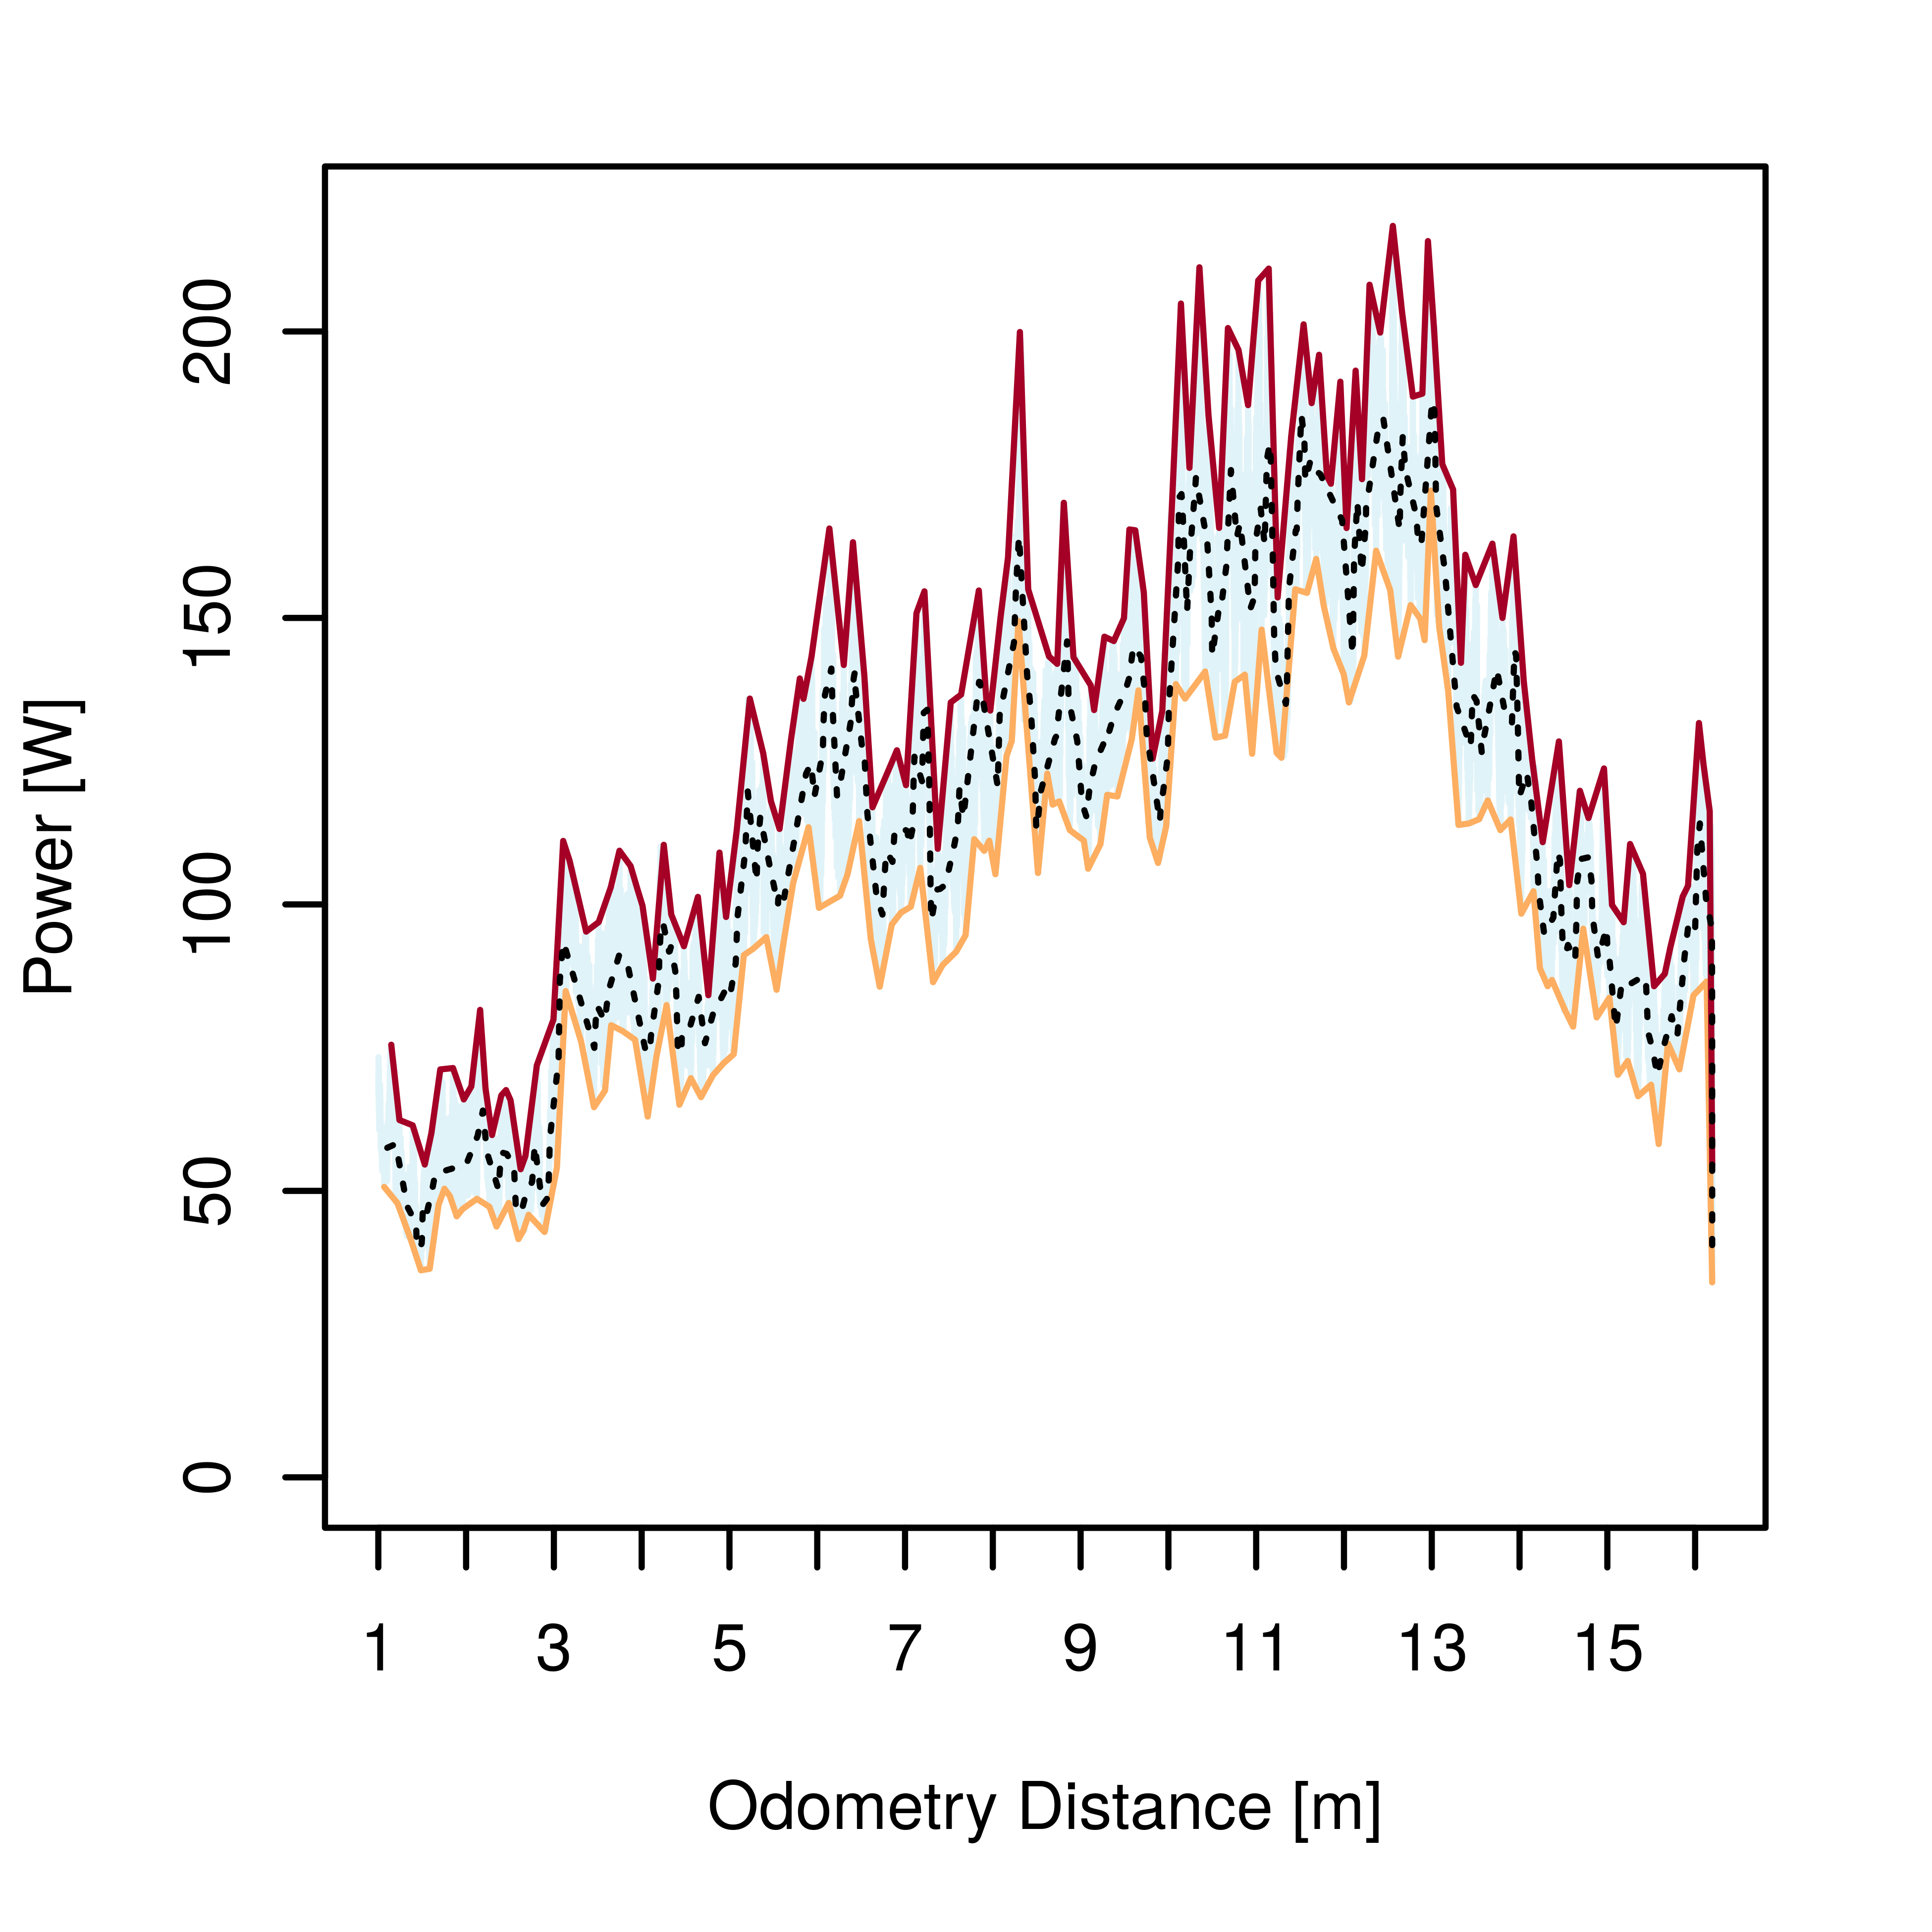
\includegraphics[height=\graphicsHeight]{sections/locomotion-power-draws/plots/locomotion-power-draw-on-upslope-terrain.png}
  		\subcaption{Propulsion}
		\label{fig:plot:sub:sherpatt-disaggregated-upslope-terrain-power-draw-locomotion}
	\end{subfigure}\hfill
	\begin{subfigure}[t]{\subfigureWidth}
        \centering
        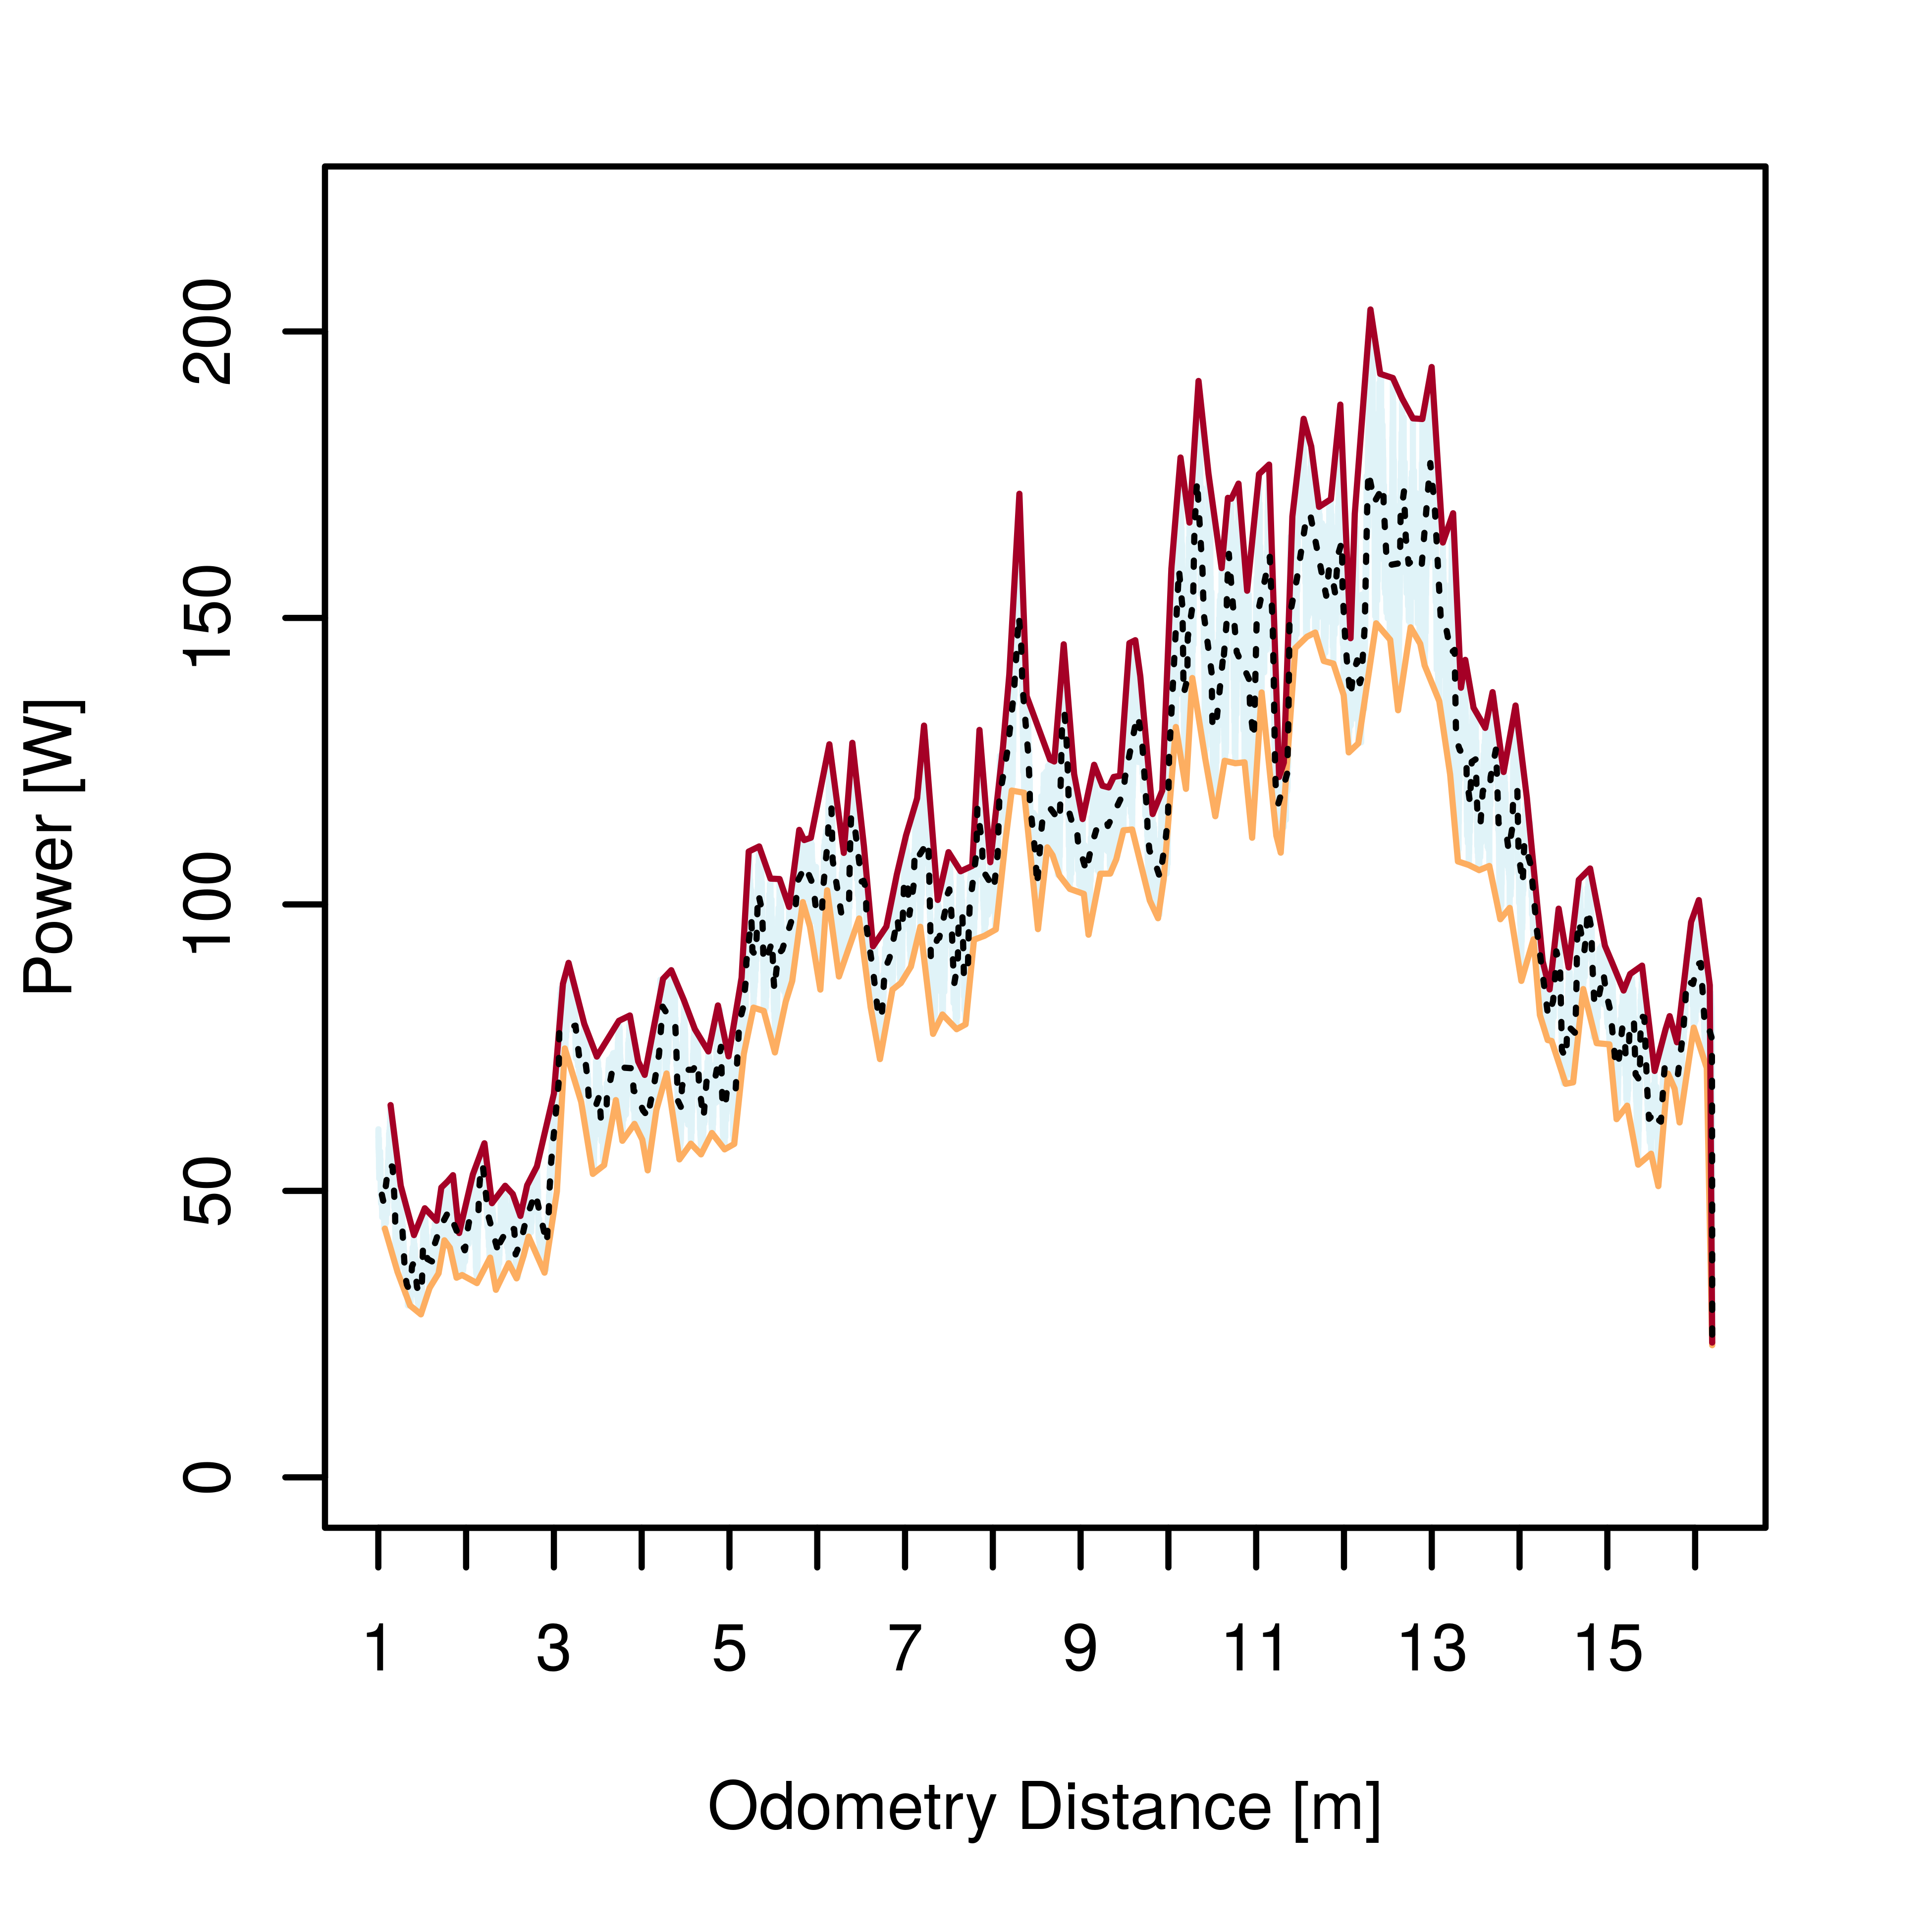
\includegraphics[height=\graphicsHeight]{sections/locomotion-power-draws/plots/drive-power-draw-on-upslope-terrain.png}
  		\subcaption{Drive}
		\label{fig:plot:sub:sherpatt-disaggregated-upslope-terrain-power-draw-drive}
	\end{subfigure}\hfill
    \begin{subfigure}[t]{\subfigureWidth}
        \centering
        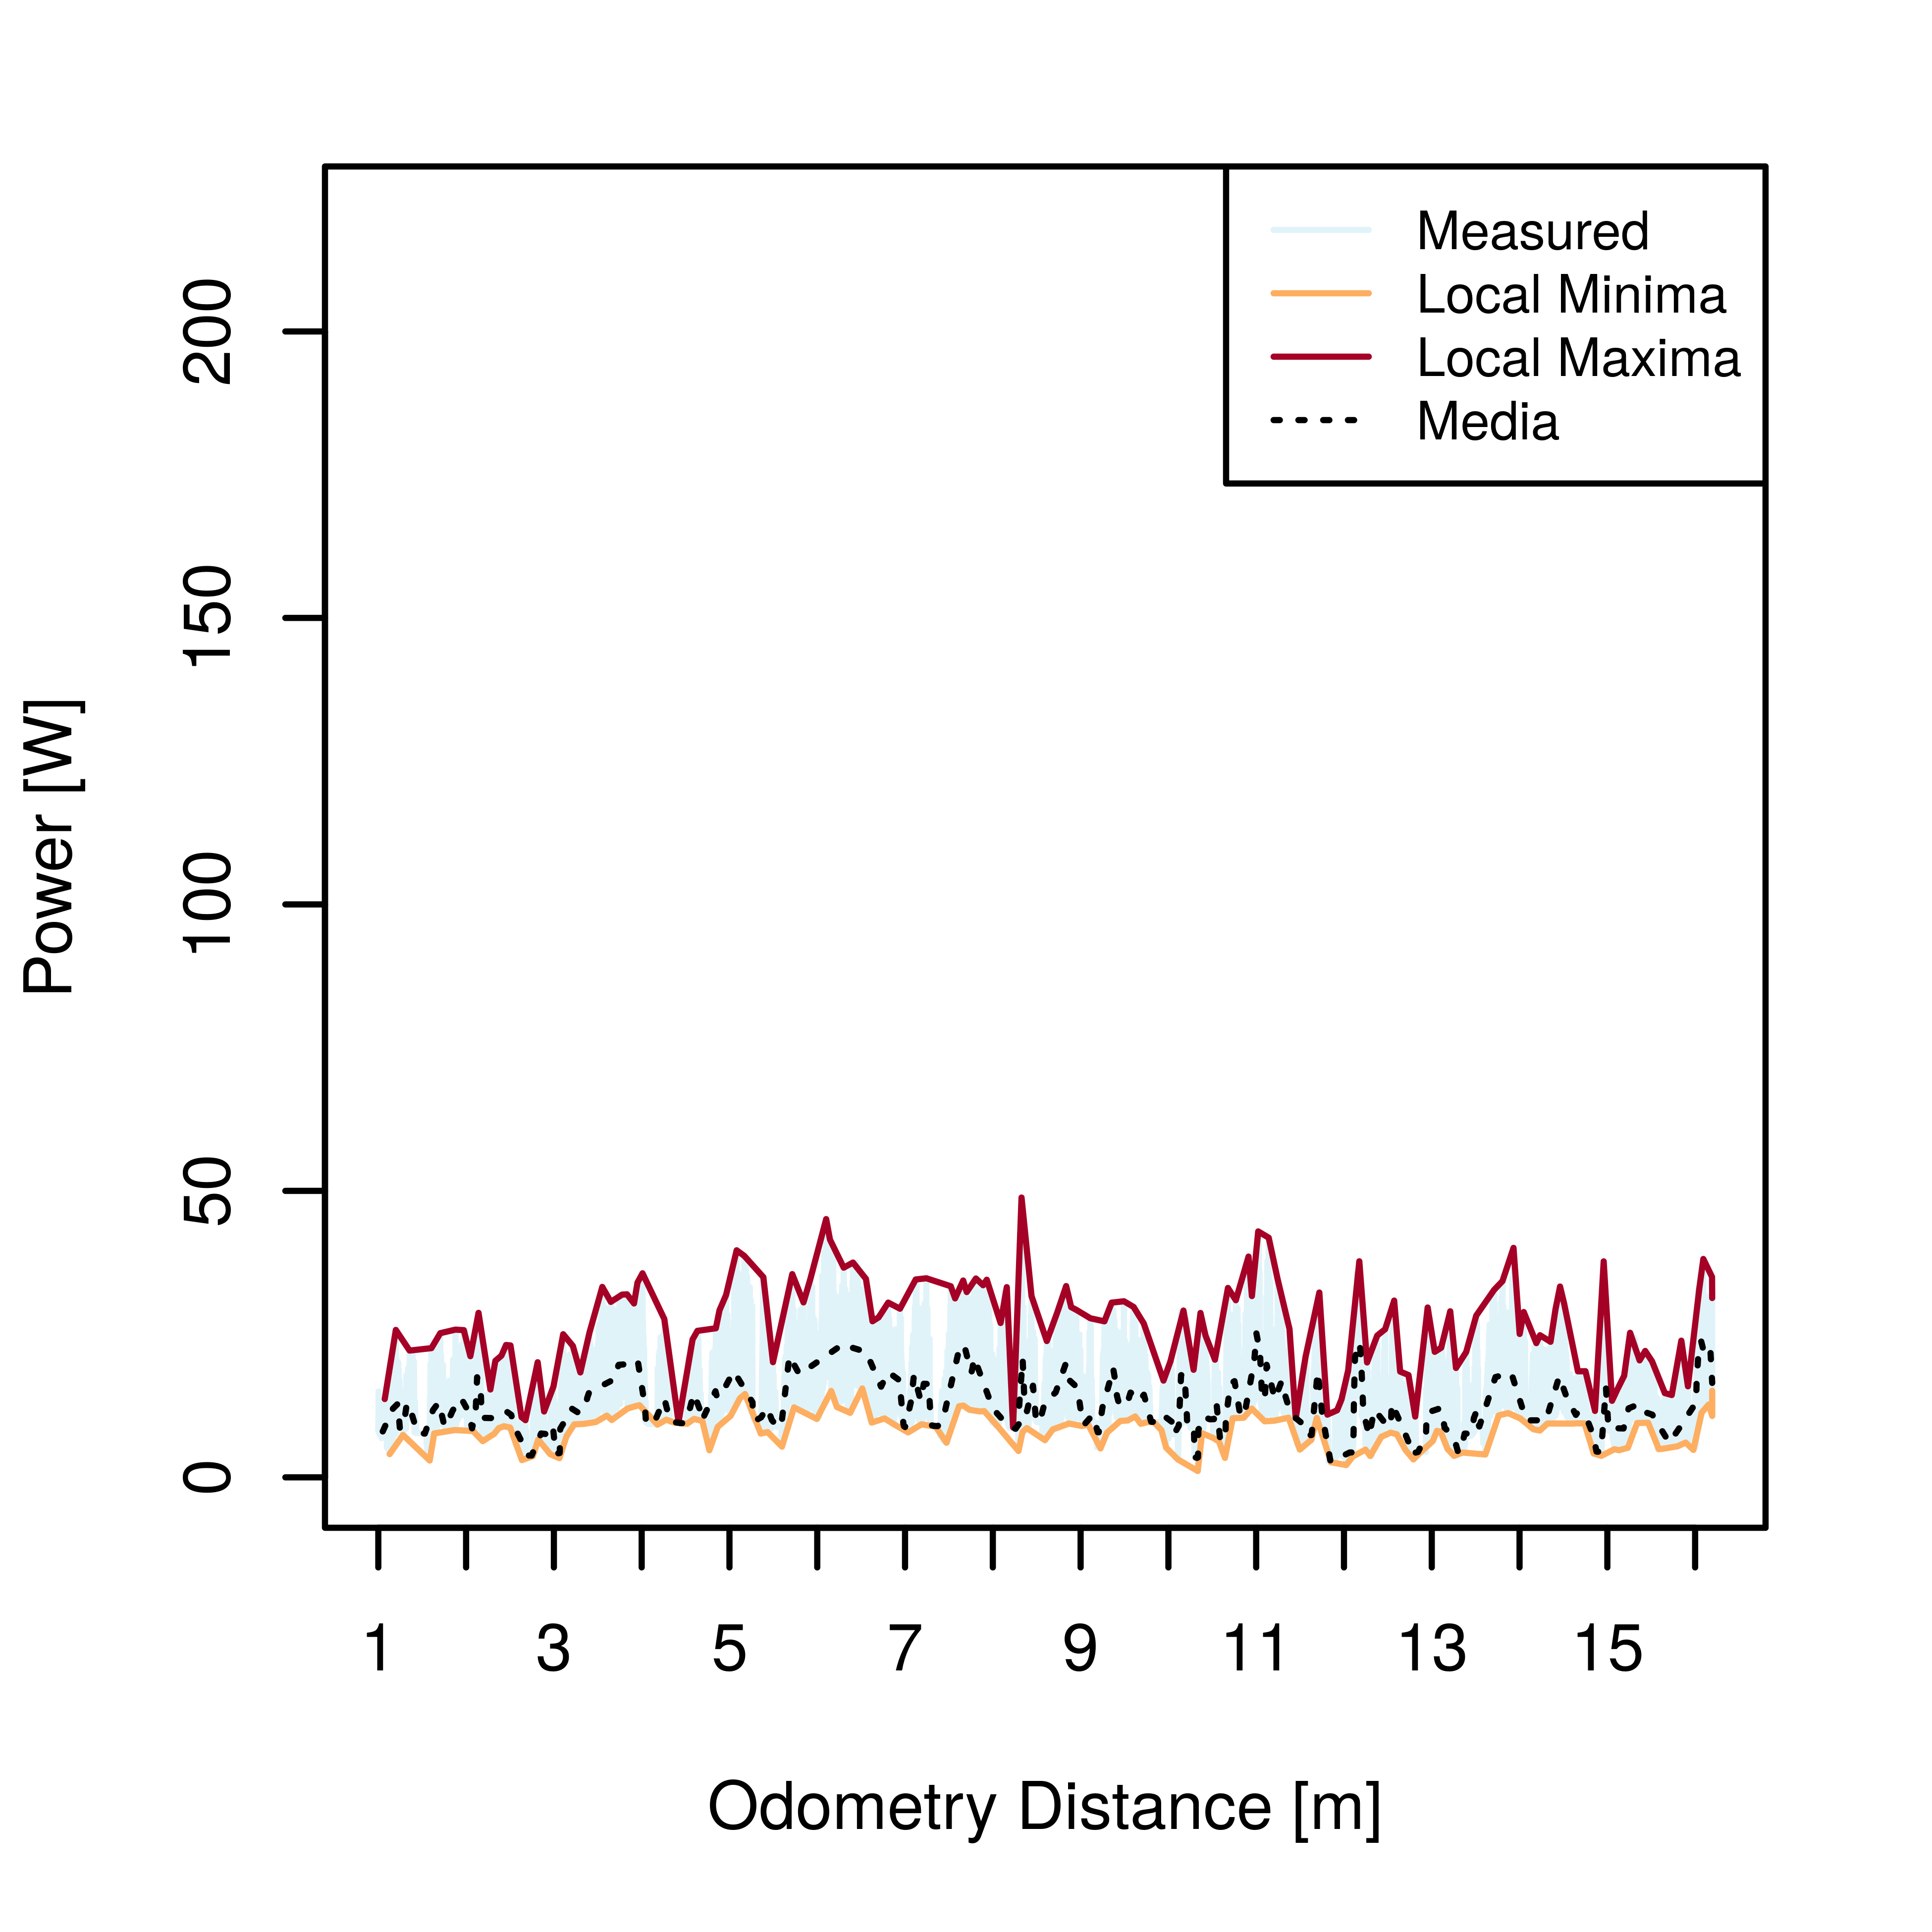
\includegraphics[height=\graphicsHeight]{sections/locomotion-power-draws/plots/suspension-power-draw-on-upslope-terrain.png}
  		\subcaption{Suspension}
		\label{fig:plot:sub:sherpatt-disaggregated-upslope-terrain-power-draw-suspension}
	\end{subfigure}\\[0.8ex]
    \caption[Disaggregated measurements of power draw for upslope terrain traverse during SherpaTT Mars analogue field tests in Utah]
            {Disaggregated measurements of power draw for upslope terrain traverse during SherpaTT Mars analogue field tests in Utah.}
    \label{fig:plot:sherpatt-disaggregated-upslope-terrain-power-draw}
\vspace{-2ex}
\end{figure}

An uplsope traverse has no discernable effect on the suspension power draw, however; there is a clear gradual increase in the drive power draw. The global maximum, minimum, and medium of the traced local minima, maxima, and media power draw lines are presented in Table \ref{tab:sherpatt-upslope-terrain-global-minimum-maximum-and-medium-power-draws}.

\clearpage
\begin{table}[h]
\centering
\caption{Global minimum, maximum, and medium of traced local minima, maxima, and media for SherpaTT upslope terrain traverse propulsion power draw lines.}
\label{tab:sherpatt-upslope-terrain-global-minimum-maximum-and-medium-power-draws}
\begin{tabular}{l|c|c|c|}
\cline{2-4}
\multicolumn{1}{c|}{\multirow{2}{*}{\textbf{}}} & \multicolumn{3}{c|}{\textbf{Power Draw {[}W{]}}} \\ \cline{2-4}
\multicolumn{1}{c|}{} & \textbf{\begin{tabular}[c]{@{}c@{}}Global Minimum\end{tabular}} & \textbf{\begin{tabular}[c]{@{}c@{}}Global Maximum\end{tabular}} & \textbf{\begin{tabular}[c]{@{}c@{}}Global Media\end{tabular}} \\ \hline
\multicolumn{1}{|l|}{\textbf{Measured}} & 34 & 218 & 114 \\ \hline
\multicolumn{1}{|l|}{\textbf{Local Minima}} & 34 & 172 & 98 \\ \hline
\multicolumn{1}{|l|}{\textbf{Local Maxima}} & 54 & 218 & 133 \\ \hline
\multicolumn{1}{|l|}{\textbf{Local Media}} & 40 & 188 & 18 \\ \hline
\end{tabular}
\end{table}


Figure \ref{fig:plot:sherpatt-upslope-terrain-power-draw} overlaps the propulsion local media power draws with the tackled slope angles. The steepest slope angle was \SI{28}{\degree} for an average of \SI{17.52}{\degree}. Slope angle increase are consistently followed by power draw spikes, i.e. at approximately 3, 4, 5, 6, 8, and 9 meters in the odometry measurements. Inversely, slope angle decreases were followed by power draws troughs at approximately 11, 13, 14, and 16 meters.

\begin{figure}[h]
  \centering
  \hypersetup{linkcolor=captionTextColor}
  \includegraphics[width=0.8\linewidth]{sections/locomotion-power-draws/plots/minima-locomotion-power-draws-on-upslope-terrain.png}\\
  \caption[Mean Propulsion power draw for an upslope terrain traverse during SherpaTT Utah field test campaign.]
          {Mean Propulsion power draw for an upslope terrain traverse during SherpaTT Utah field test campaign.}
  \label{fig:plot:sherpatt-upslope-terrain-power-draw}
\end{figure}

The power draws trough following the slope angle change from \SI{28}{\degree} to \SI{20}{\degree} at the \SI{11}{\meter} mark is subsequently followed by an unusual power draw increase and fluctuation. These measurements were discarded as they are outliers with respect to the power draw responses for the slope angle descreases that followed.

Table \ref{tab:sherpatt-upslope-terrain-local-media-measurement-summary} summarises the minimum, maximum, and mean local media propulsion power draws that were measured for different slope angles. Discarding the outlier measurements subsequent to the slope angle change from \SI{28}{\degree} to \SI{20}{\degree} at the \SI{11}{\meter} to \SI{13}{\meter} portion of the track, the maximum mean local media propulsion power draw is \SI{146}{\watt}.

\clearpage
\begin{table}[h]
\centering
\caption{SherpaTT mean propulsion power draw measurements for different slope sections}
\label{tab:sherpatt-upslope-terrain-local-media-measurement-summary}
\begin{tabular}{cc|c|c|c|}
\cline{3-5}
\multicolumn{1}{l}{} & \multicolumn{1}{l|}{} & \multicolumn{3}{c|}{\textbf{Power {[}W{]}}} \\ \hline
\multicolumn{1}{|l|}{\textbf{Distance {[}m{]}}} & \multicolumn{1}{l|}{\textbf{Slope Angle {[}deg{]}}} & \multicolumn{1}{l|}{\textbf{Minimum}} & \multicolumn{1}{l|}{\textbf{Maximum}} & \multicolumn{1}{l|}{\textbf{Mean}} \\ \hline
\multicolumn{1}{|c|}{\textbf{1 $<$ x $\leq$ 3}} & 10 & 40 & 64 & 51 \\ \hline
\multicolumn{1}{|c|}{\textbf{3 $<$ x $\leq$ 4}} & 11 & 73 & 93 & 85 \\ \hline
\multicolumn{1}{|c|}{\textbf{4 $<$ x $\leq$ 5}} & 15 & 74 & 87 & 83 \\ \hline
\multicolumn{1}{|c|}{\textbf{5 $<$ x $\leq$ 6}} & 16 & 85 & 125 & 107 \\ \hline
\multicolumn{1}{|c|}{\textbf{6 $<$ x $\leq$ 7}} & 28 & 98 & 141 & 123 \\ \hline
\multicolumn{1}{|c|}{\textbf{7 $<$ x $\leq$ 8}} & 22 & 97 & 139 & 116 \\ \hline
\multicolumn{1}{|c|}{\textbf{8 $<$ x $\leq$ 9}} & 25 & 113 & 164 & 133 \\ \hline
\multicolumn{1}{|c|}{\textbf{9 $<$ x $\leq$ 11}} & 28 & 114 & 176 & 146 \\ \hline
\multicolumn{1}{|c|}{\textbf{11 $<$ x $\leq$ 13}} & 20 & 135 & 188 & 167 \\ \hline
\multicolumn{1}{|c|}{\textbf{13 $<$ x $\leq$ 14}} & 15 & 119 & 123 & 145 \\ \hline
\multicolumn{1}{|c|}{\textbf{14 $<$ x $\leq$ 16}} & 10 & 70 & 186 & 94 \\ \hline
\end{tabular}
\end{table}


\section{Conclusion}
\label{sec:PropulsionPowerConstraints:Conclusion}
Based on data from the SherpaTT field campaign and the assumptions made in Section \ref{sec:PropulsionPowerConstraints:Introduction}, the following power subsystem requirements were proposed with respect to propulsion power draws:

\begin{itemize}
    \item The rover shall provide up to \SI{75}{\watt} in propulsion power for flat terrain traverses.
    \item The rover shall provide up to \SI{150}{\watt} in propulsion power for upslope terrain traverses of up to \SI{30}{\degree} inclination.
\end{itemize}


\clearpage
\section{Solar Array}
\label{sec:Design:SolarArray}
\section{Introduction}
\label{sec:PropulsionPowerConstraints:Introduction}
SherpaTT's actively articulated suspension system consists of 4 wheeled-legs with a total of 20 motors. Each leg is equipped with 3 suspension motors and 2 drive motors. The suspension motors are responsible for Pan, \ac{IL}, and \ac{OL} revolute joint rotations whereas the drive motors are responsible for \ac{WS} and \ac{WD}. The distribution of these motors across each leg are shown in Figure \ref{fig:sherpatt-actively-articulated-suspension-system}. Propulsion power draw refers to the summation of suspension and drive motor power draws. These power draws have been studied in detail for SherpaTT during a Mars analogue field campaign in Utah \citeother{Cordes2018}.

\begin{figure}[h]
  \centering
  \hypersetup{linkcolor=captionTextColor}
  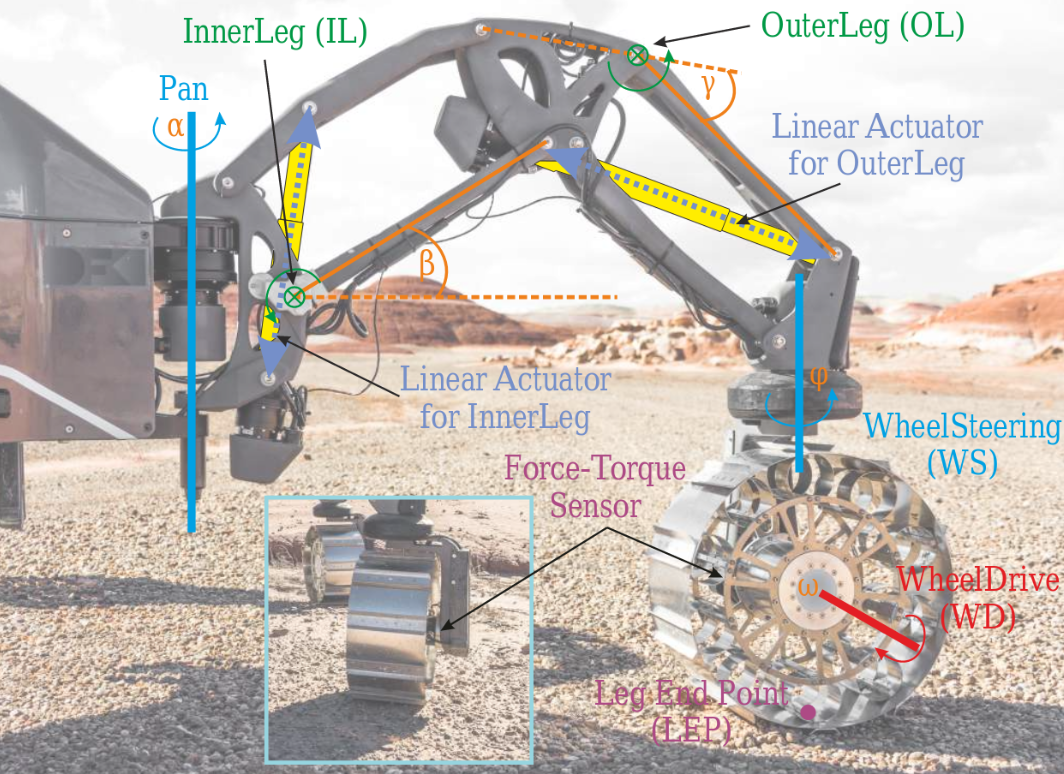
\includegraphics[width=0.8\linewidth]{sections/locomotion-power-draws/images/sherpatt-actively-articulated-suspension-sytem.png}\\
  \caption[SherpaTT actively articulated suspension system]
          {SherpaTT actively articulated suspension system.}
  \label{fig:sherpatt-actively-articulated-suspension-system}
\end{figure}

 This section restricts power draw analysis to establishing propulsion power constraints for the study of SherpaTT Mars mission scenarios. Lack of motor optimisation as well as lower gravity and pressure on Mars permit the assumption that, given similar topology traversals, measured propulsion power draws are greater than those that would be observed on a Martian environment. This assumption is further supported when considering that SherpaTT's velocities during power draw measurements were much greater than what has been achieved on present and past Mars rover missions.


\section{Power Draw}
\label{sec:PropulsionPowerConstraints:PowerDraw}
Available datasets from the Mars analogue field test campaign cover 2 flat surface runs and 3 steep upslope terrain runs. From the 2 upslope runs, the dataset with the worst-case maximum and mean propulsion power draw was used as the worst-case scenario. Hereafter, all mention of SherpaTT power draws will reference measurements included in these datasets. Measured power draws fluctuate due to slips, skids, noise, and other unknown imperfections. To ease readability, local minima, maxima, and media lines have been traced for all power plot figures.


\subsection{Flat Terrain Traverse}
\label{sec:PropulsionPowerConstraints:FlatTerrainTraverse}
\ac{MER} and \ac{MSL} rovers are each equipped with a total of 10 propulsion motors to drive their Rocker-Bogie passive suspension system: 6 to rotate the wheels and 4 to steer them \citeother{Novak2005} \citeother{Lakdawalla2018}. The \ac{MER} rovers needed approximately \SI{100}{\watt} to drive \citeother{MERRoverEnergy}. Propulsion power draws measured for SherpaTT on flat surface runs are shown in Figure \ref{fig:plot:sherpatt-flat-terrain-power-draw}.

\begin{figure}[h]
\captionsetup[subfigure]{justification=centering}
\vspace{-2ex}
	\centering
    %% setup sizes
    \setlength{\subfigureWidth}{0.50\textwidth}
    \setlength{\graphicsHeight}{80mm}
    %% kill hyper-link highlighting
    \hypersetup{hidelinks=true}%
    %% the figures
    \begin{subfigure}[t]{\subfigureWidth}
        \centering
        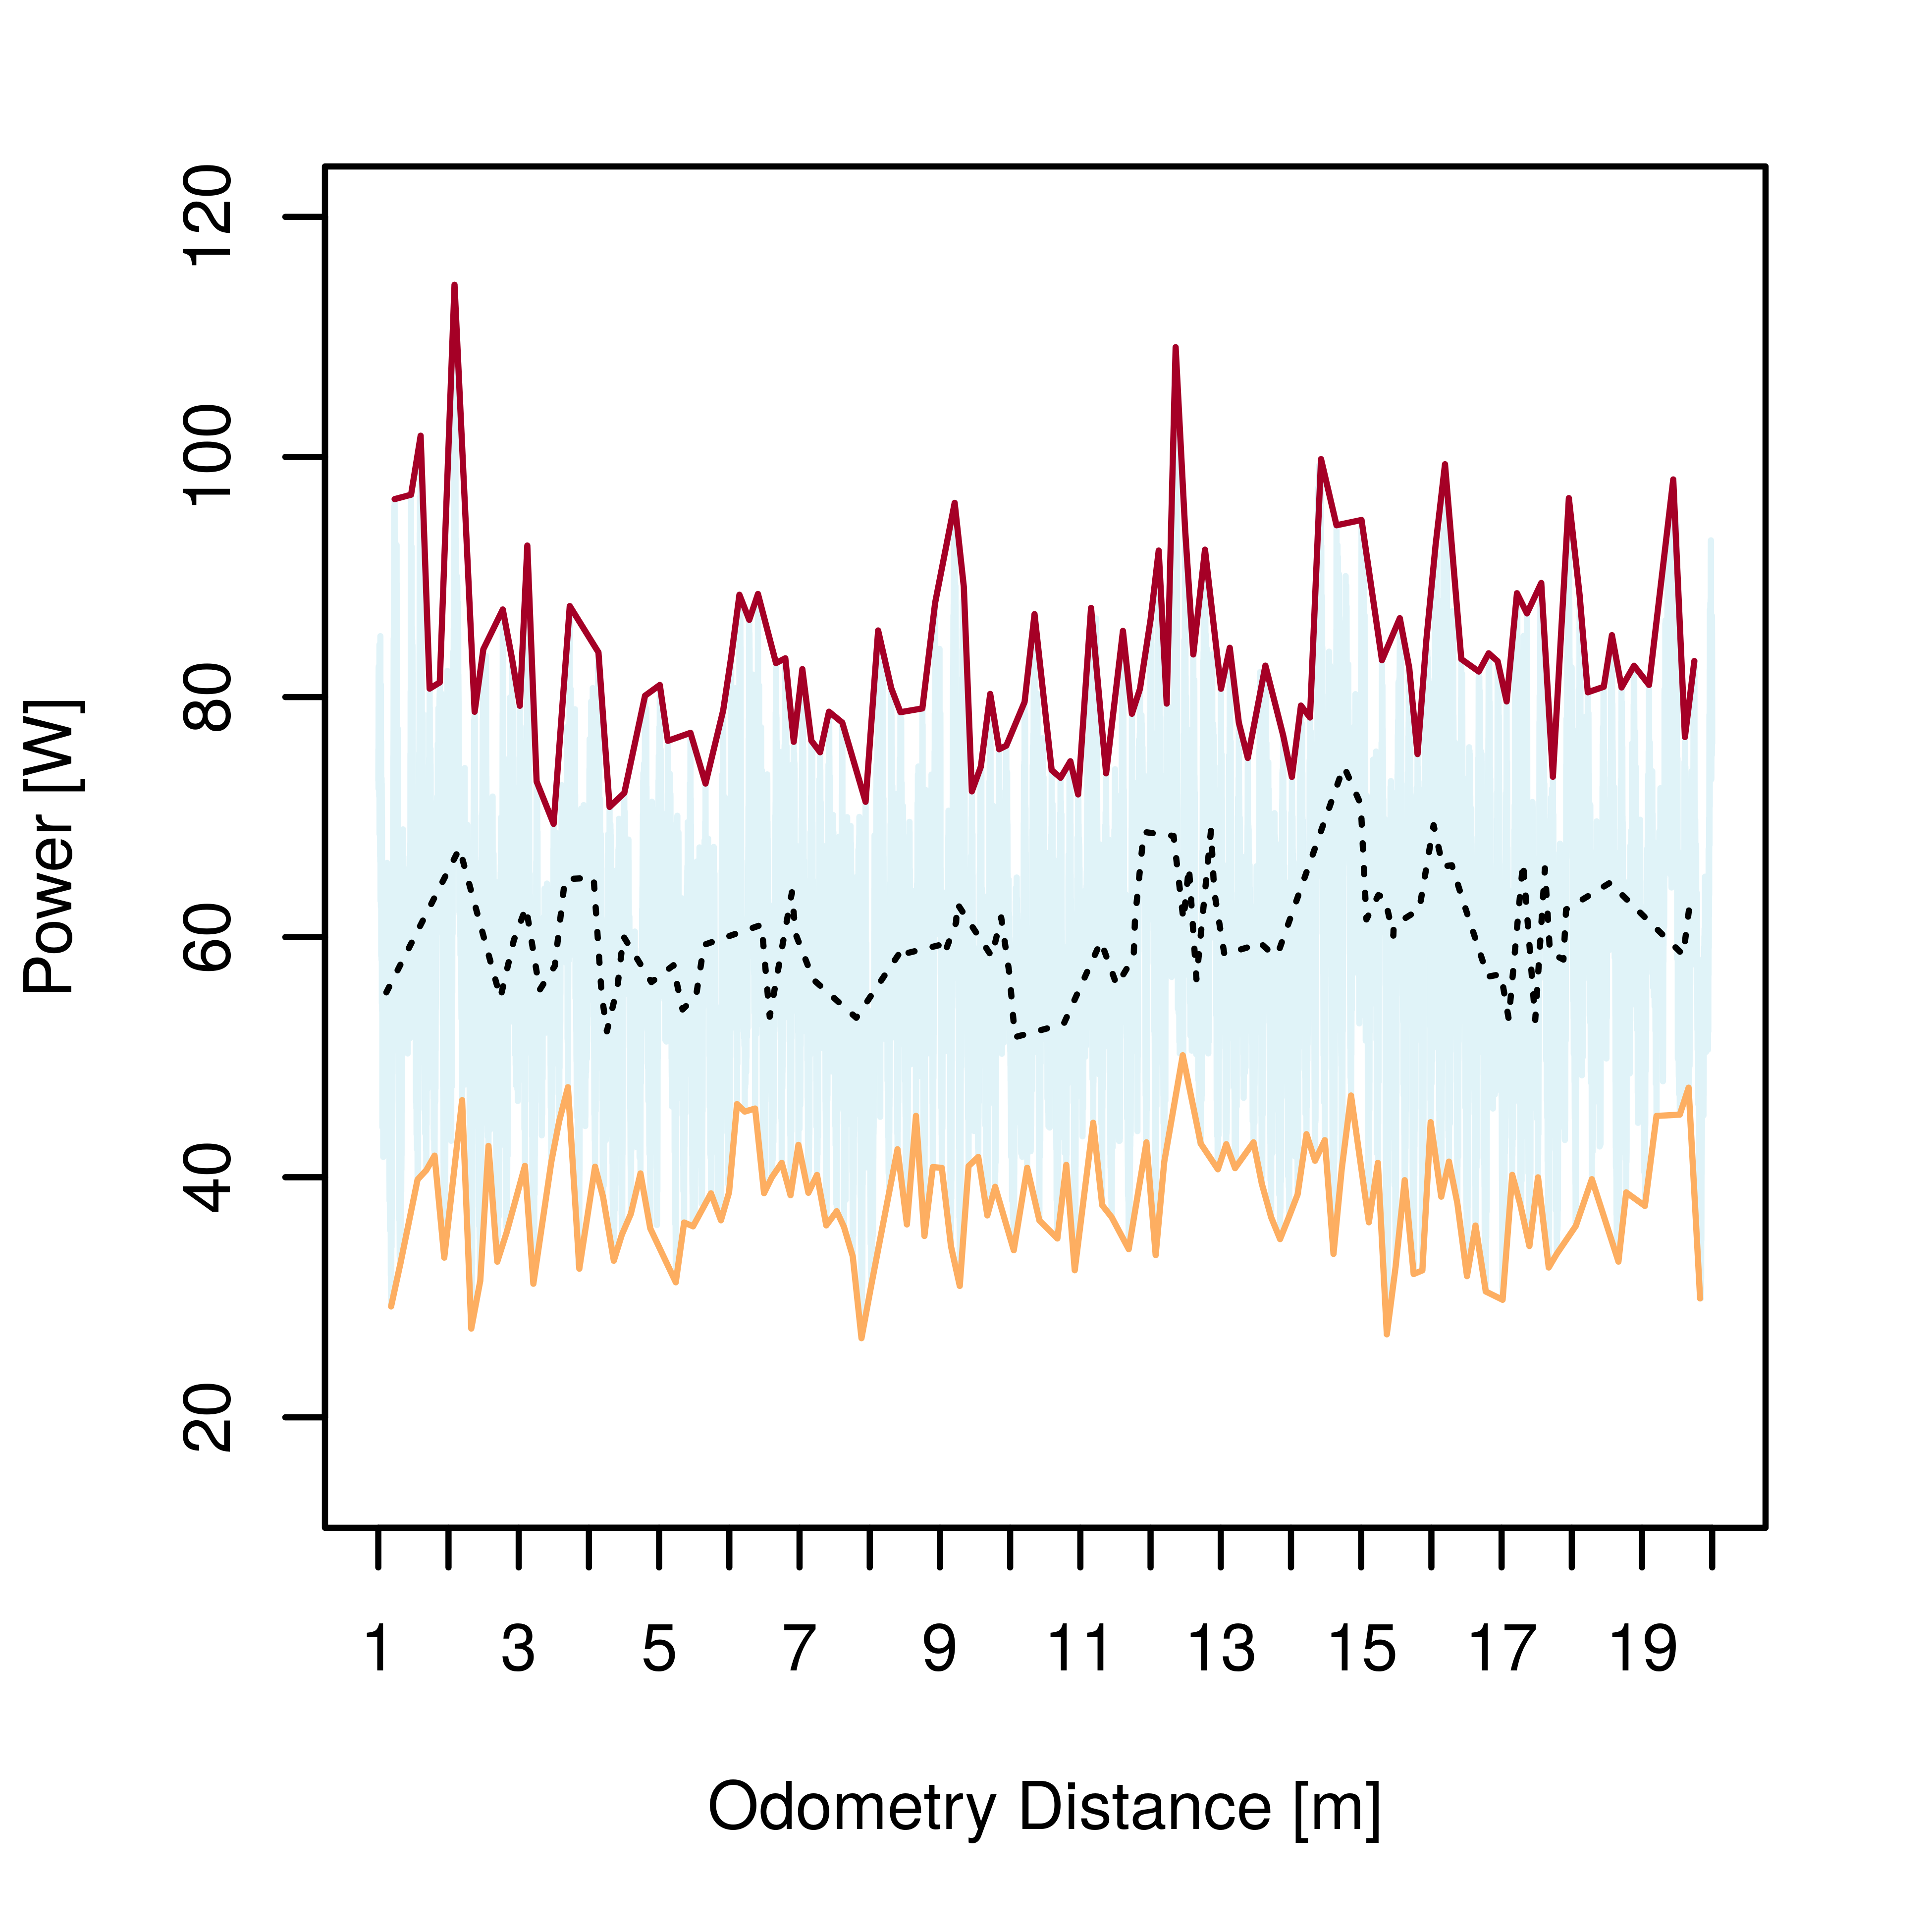
\includegraphics[height=\graphicsHeight]{sections/locomotion-power-draws/plots/locomotion-power-draw-on-flat-terrain-1.png}
        \subcaption{Run \#1}
        \label{fig:plot:sub:sherpatt-flat-terrain-power-draw-1}
    \end{subfigure}\hfill
    \begin{subfigure}[t]{\subfigureWidth}
        \centering
        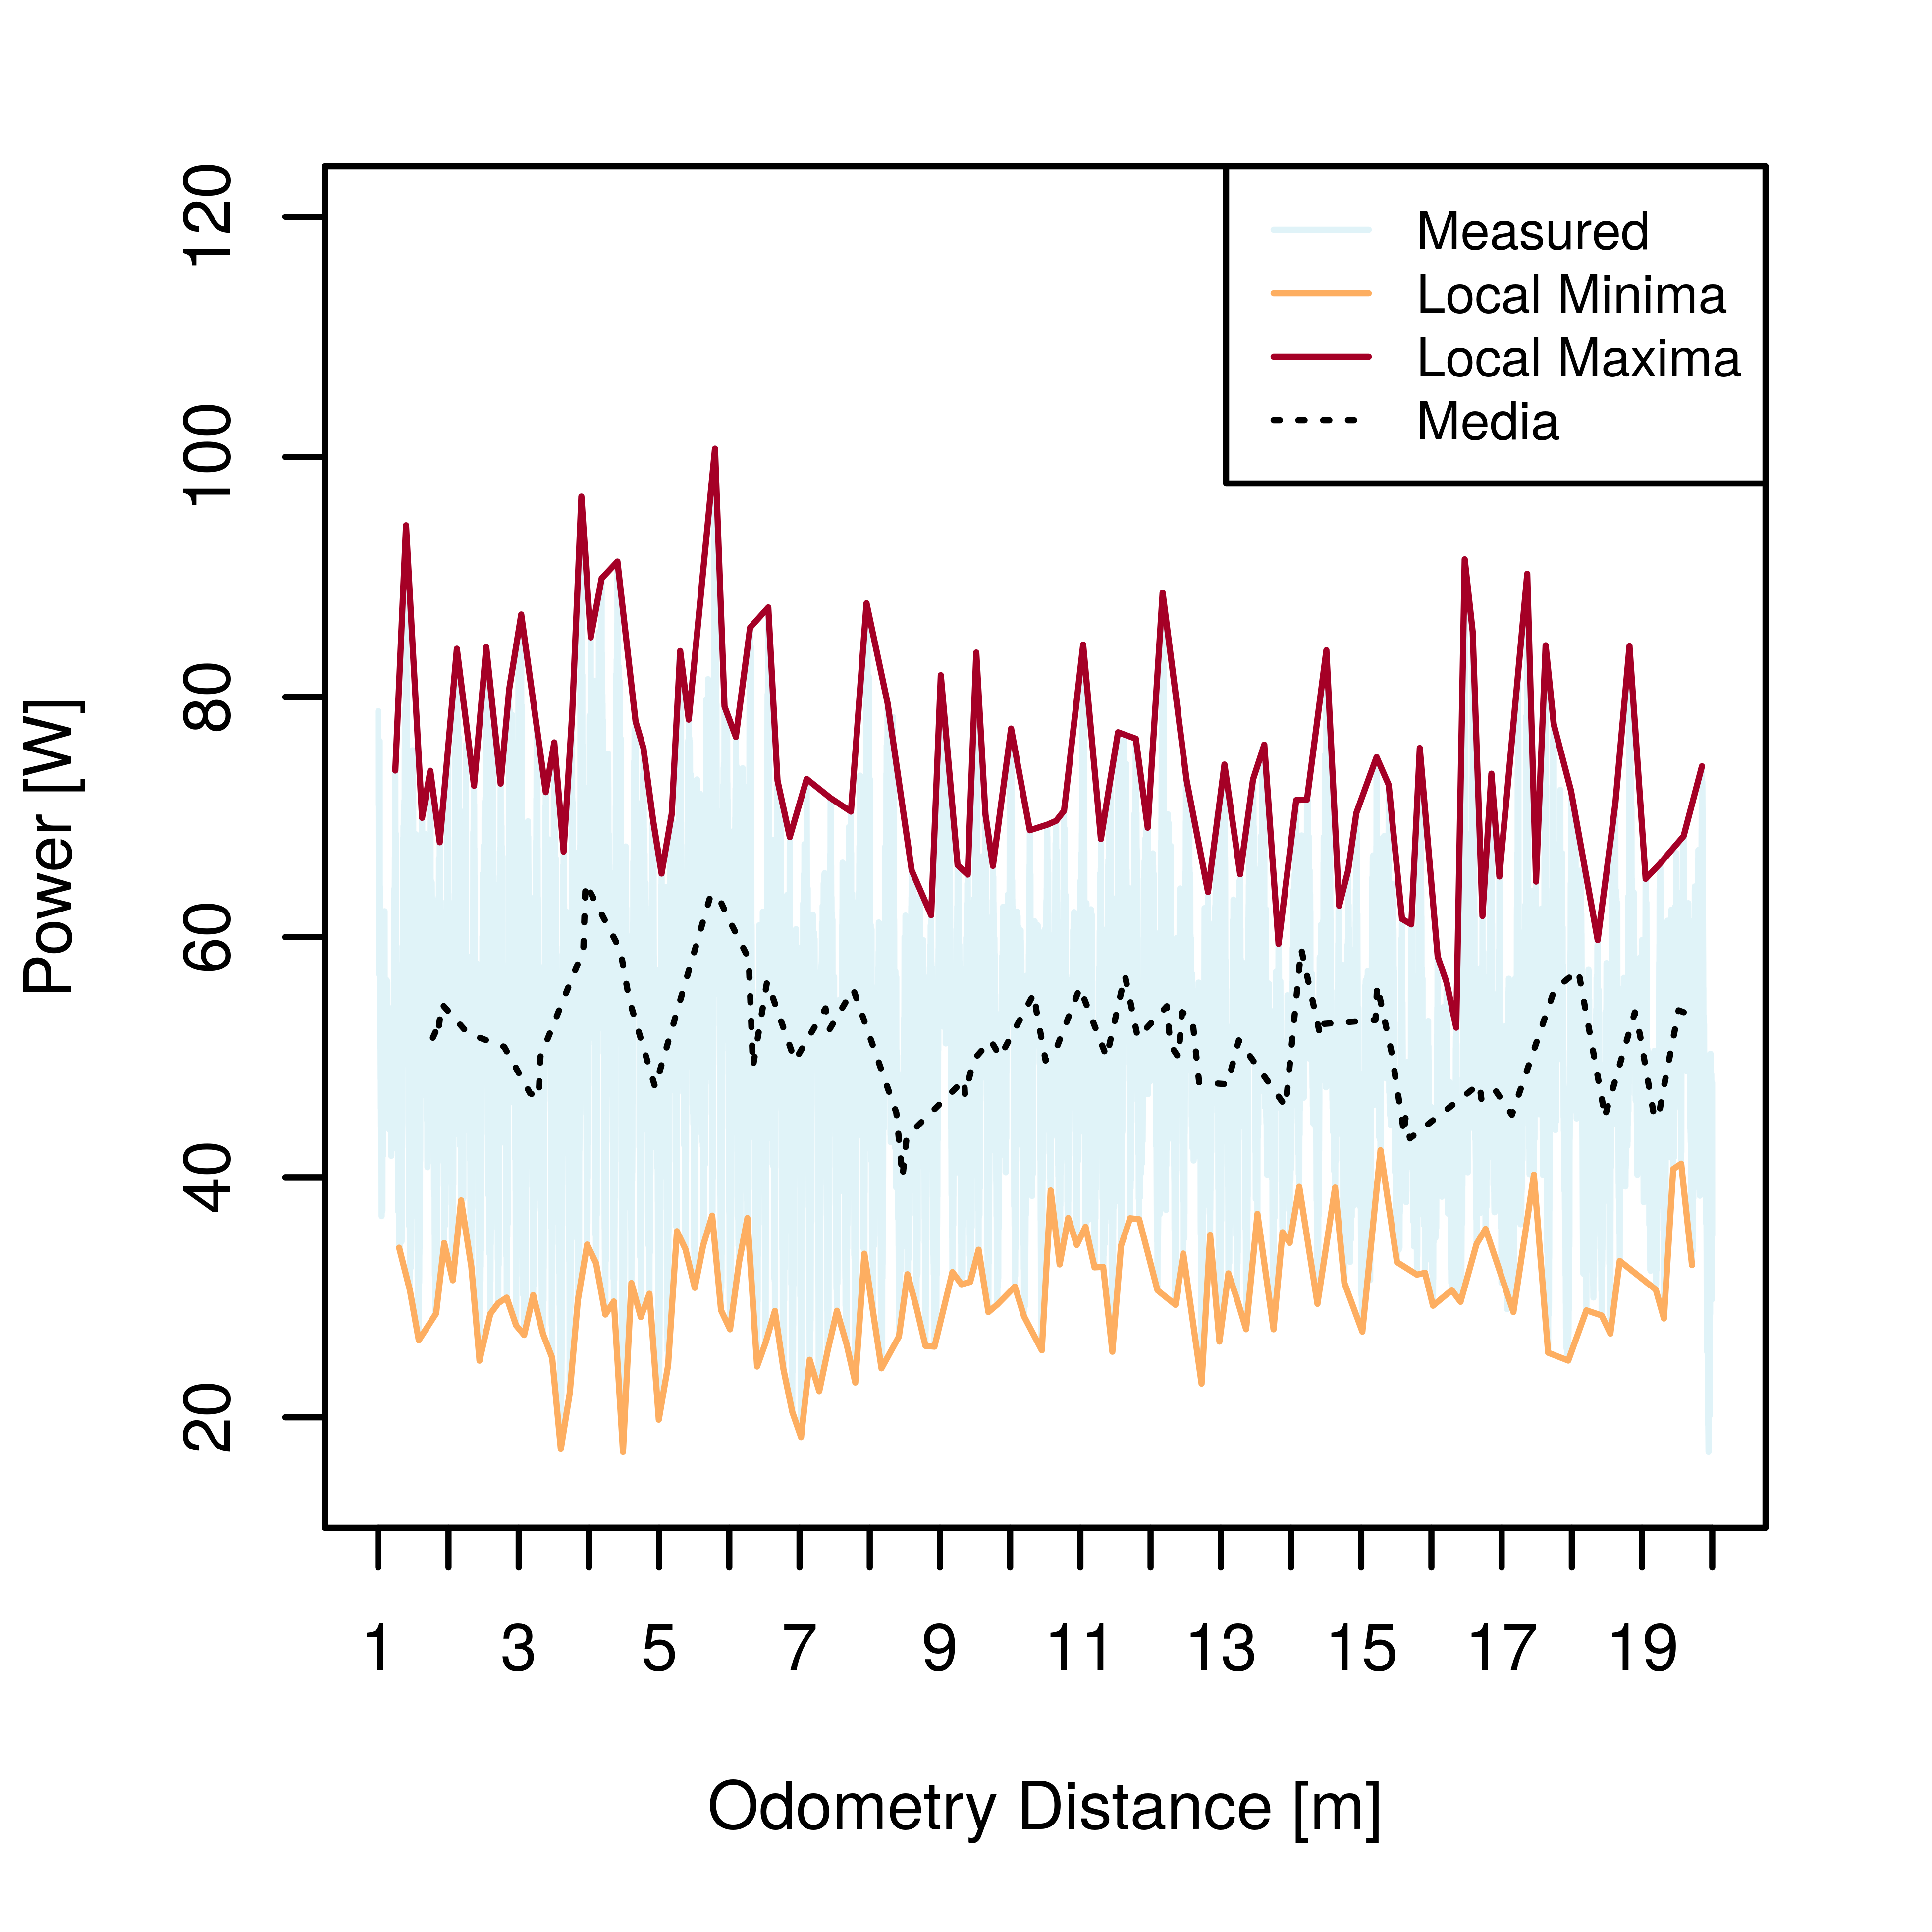
\includegraphics[height=\graphicsHeight]{sections/locomotion-power-draws/plots/locomotion-power-draw-on-flat-terrain-2.png}
  		\subcaption{Run \#2}
		\label{fig:plot:sub:sherpatt-flat-terrain-power-draw-2}
	\end{subfigure}\\[0.8ex]
    \caption[Propulsion power draw for a flat terrain traverse during SherpaTT Mars analogue field tests in Utah]
            {Propulsion power draw for a flat terrain traverse during SherpaTT Mars analogue field tests in Utah.}
    \label{fig:plot:sherpatt-flat-terrain-power-draw}
\vspace{-2ex}
\end{figure}


These measurements are summarised in Table \ref{tab:sherpatt-flat-terrain-global-minimum-maximum-and-medium-power-draws}. To eliminate power draw fluctuations from the analysis, only local media values were considered. Local media were selected rather than the worst-case local maxima on the basis of the assumptions made in Section \ref{sec:PropulsionPowerConstraints:Introduction}. For flat terrain traverses, a worst-case maximum power draw of \SI{74}{\watt} is observed for a mean of \SI{61}{\watt}.

\clearpage
\begin{table}[h]
\centering
\caption{Global minimum, maximum, and medium of traced local minima, maxima, and media for SherpaTT flat terrain propulsion power draw lines.}
\label{tab:sherpatt-flat-terrain-global-minimum-maximum-and-medium-power-draws}
\begin{tabular}{llccc}
\cline{3-5}
\multicolumn{2}{l|}{\multirow{2}{*}{}} & \multicolumn{3}{c|}{\textbf{Power Draw {[}W{]}}} \\ \cline{3-5}
\multicolumn{2}{l|}{} & \multicolumn{1}{c|}{\textbf{\begin{tabular}[c]{@{}c@{}}Global Minimum\end{tabular}}} & \multicolumn{1}{c|}{\textbf{\begin{tabular}[c]{@{}c@{}}Global Maximum\end{tabular}}} & \multicolumn{1}{c|}{\textbf{\begin{tabular}[c]{@{}c@{}}Global Media\end{tabular}}} \\ \hline
\multicolumn{1}{|c|}{\multirow{4}{*}{\textbf{Run \#1}}} & \multicolumn{1}{l|}{\textbf{Measured}} & \multicolumn{1}{c|}{27} & \multicolumn{1}{c|}{114} & \multicolumn{1}{c|}{60} \\ \cline{2-5}
\multicolumn{1}{|c|}{} & \multicolumn{1}{l|}{\textbf{Local Minima}} & \multicolumn{1}{c|}{27} & \multicolumn{1}{c|}{50} & \multicolumn{1}{c|}{38} \\ \cline{2-5}
\multicolumn{1}{|c|}{} & \multicolumn{1}{l|}{\textbf{Local Maxima}} & \multicolumn{1}{c|}{69} & \multicolumn{1}{c|}{114} & \multicolumn{1}{c|}{83} \\ \cline{2-5}
\multicolumn{1}{|c|}{} & \multicolumn{1}{l|}{\textbf{Local Media}} & \multicolumn{1}{c|}{52} & \multicolumn{1}{c|}{74} & \multicolumn{1}{c|}{61} \\ \hhline{|=|=|=|=|=|}
\multicolumn{1}{|l|}{\multirow{4}{*}{\textbf{Run \#2}}} & \multicolumn{1}{l|}{\textbf{Measured}} & \multicolumn{1}{c|}{17} & \multicolumn{1}{c|}{101} & \multicolumn{1}{c|}{51} \\ \cline{2-5}
\multicolumn{1}{|l|}{} & \multicolumn{1}{l|}{\textbf{Local Minima}} & \multicolumn{1}{c|}{17} & \multicolumn{1}{c|}{42} & \multicolumn{1}{c|}{30} \\ \cline{2-5}
\multicolumn{1}{|l|}{} & \multicolumn{1}{l|}{\textbf{Local Maxima}} & \multicolumn{1}{c|}{52} & \multicolumn{1}{c|}{101} & \multicolumn{1}{c|}{74} \\ \cline{2-5}
\multicolumn{1}{|l|}{} & \multicolumn{1}{l|}{\textbf{Local Media}} & \multicolumn{1}{c|}{40} & \multicolumn{1}{c|}{64} & \multicolumn{1}{c|}{52} \\ \hline
 &  & \multicolumn{1}{l}{} & \multicolumn{1}{l}{} & \multicolumn{1}{l}{} \\
 &  & \multicolumn{1}{l}{} & \multicolumn{1}{l}{} & \multicolumn{1}{l}{}
\end{tabular}
\end{table}


\subsection{Upslope Terrain Traverse}
\label{sec:PropulsionPowerConstraints:UpslopeTerrainTraverse}
Propulsion power draws on a steep uplsope were measured along an approximately \SI{16}{\meter} track and are shown Figure \ref{fig:plot:sub:sherpatt-disaggregated-upslope-terrain-power-draw-locomotion}. The drive and suspension power draw components are shown in Figures \ref{fig:plot:sub:sherpatt-disaggregated-upslope-terrain-power-draw-drive} and \ref{fig:plot:sub:sherpatt-disaggregated-upslope-terrain-power-draw-suspension}, respectively.

\begin{figure}[h]
\captionsetup[subfigure]{justification=centering}
\vspace{-2ex}
	\centering
    %% setup sizes
    \setlength{\subfigureWidth}{0.32\textwidth}
    \setlength{\graphicsHeight}{50mm}
    %% kill hyper-link highlighting
    \hypersetup{hidelinks=true}%
    %% the figures
	\begin{subfigure}[t]{\subfigureWidth}
        \centering
        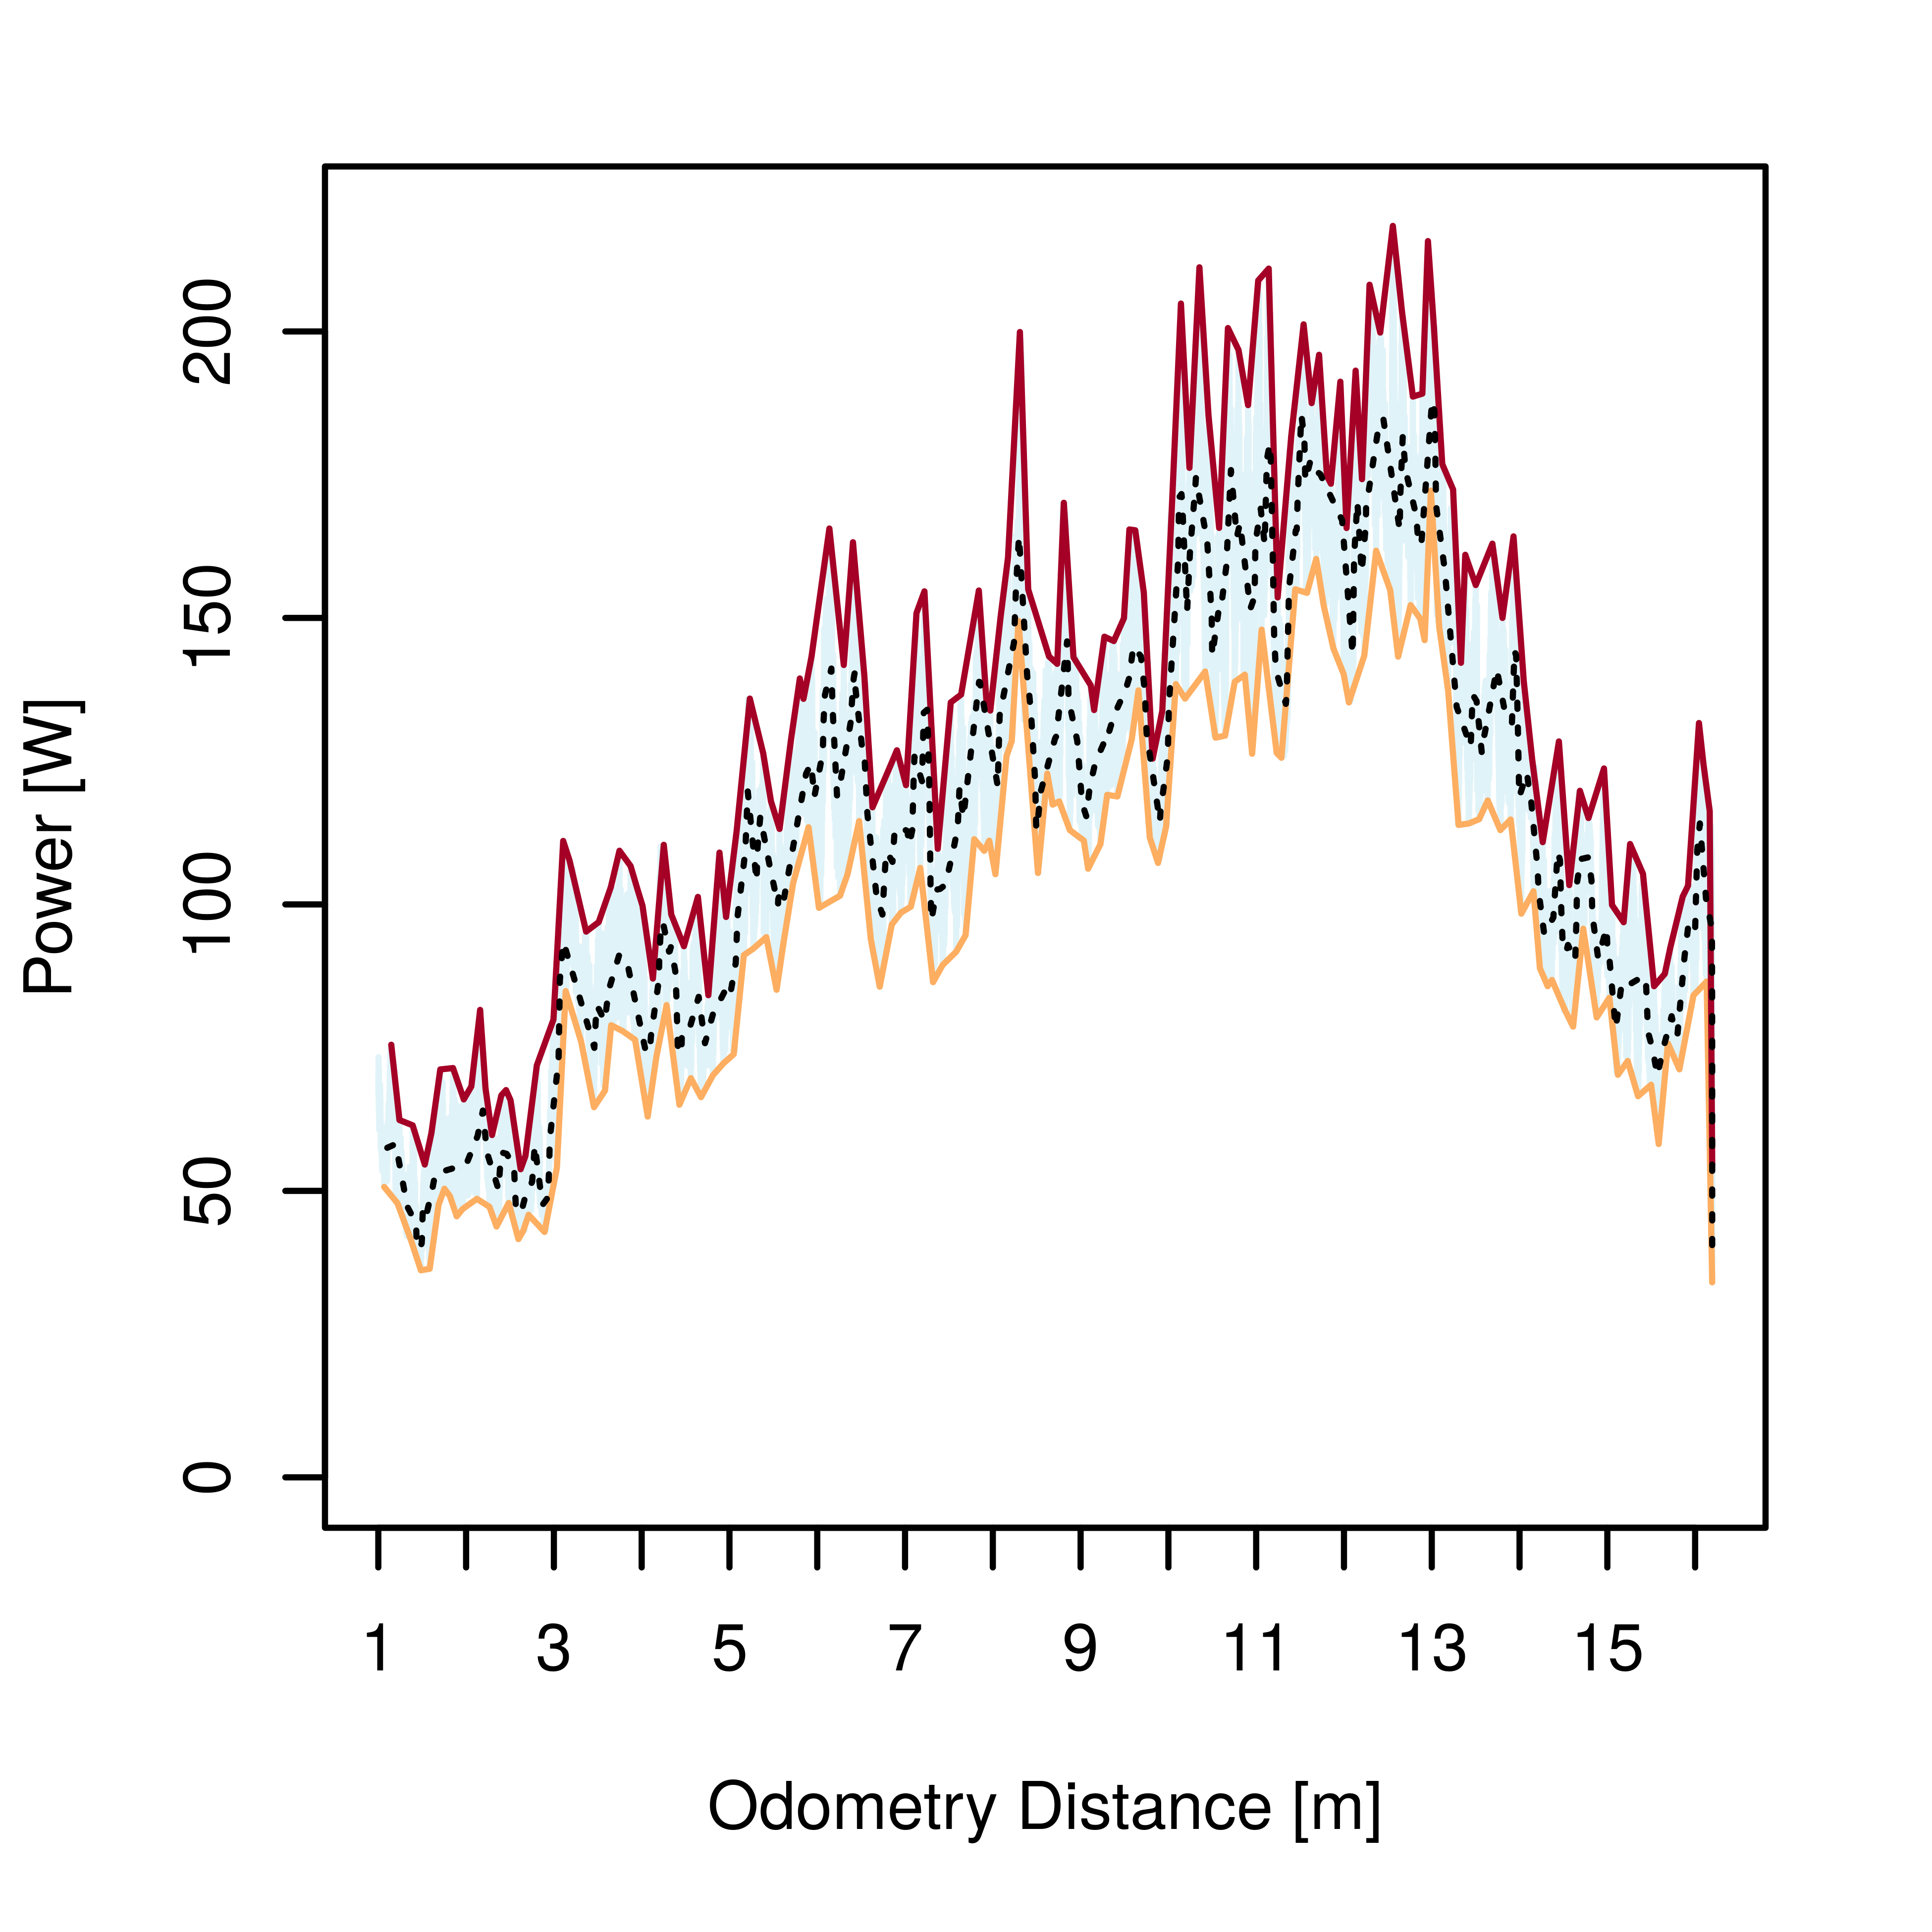
\includegraphics[height=\graphicsHeight]{sections/locomotion-power-draws/plots/locomotion-power-draw-on-upslope-terrain.png}
  		\subcaption{Propulsion}
		\label{fig:plot:sub:sherpatt-disaggregated-upslope-terrain-power-draw-locomotion}
	\end{subfigure}\hfill
	\begin{subfigure}[t]{\subfigureWidth}
        \centering
        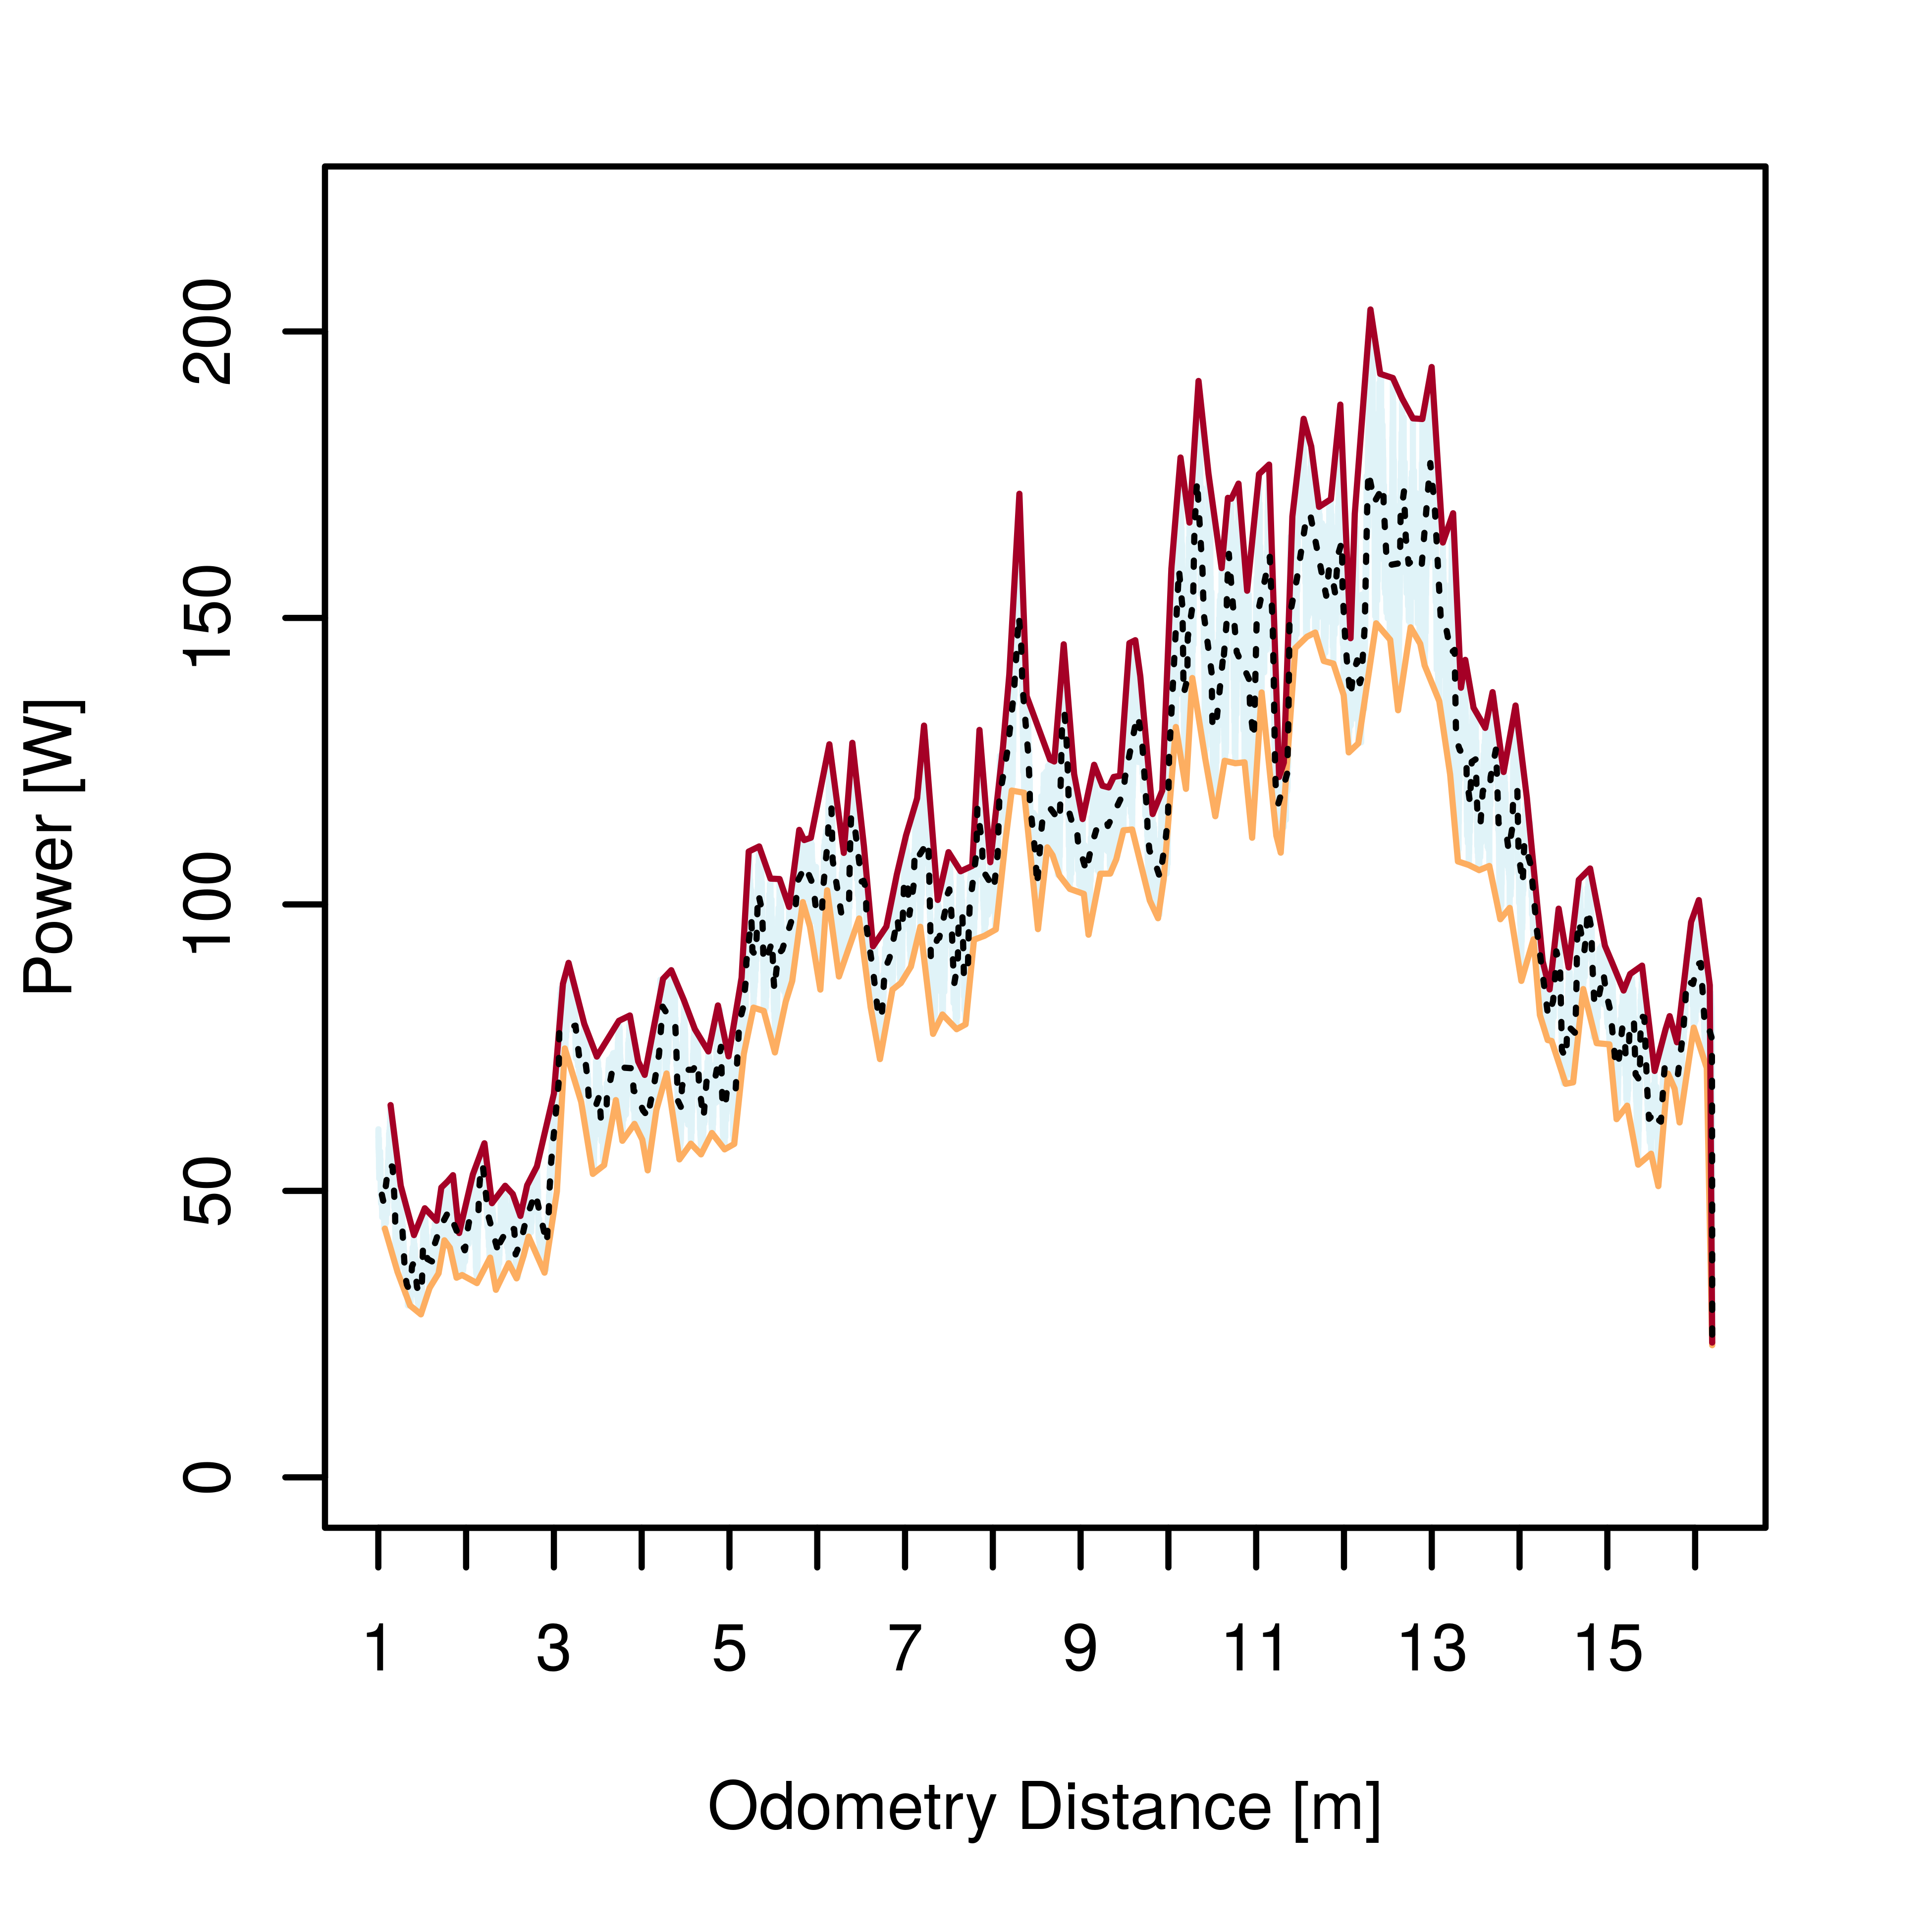
\includegraphics[height=\graphicsHeight]{sections/locomotion-power-draws/plots/drive-power-draw-on-upslope-terrain.png}
  		\subcaption{Drive}
		\label{fig:plot:sub:sherpatt-disaggregated-upslope-terrain-power-draw-drive}
	\end{subfigure}\hfill
    \begin{subfigure}[t]{\subfigureWidth}
        \centering
        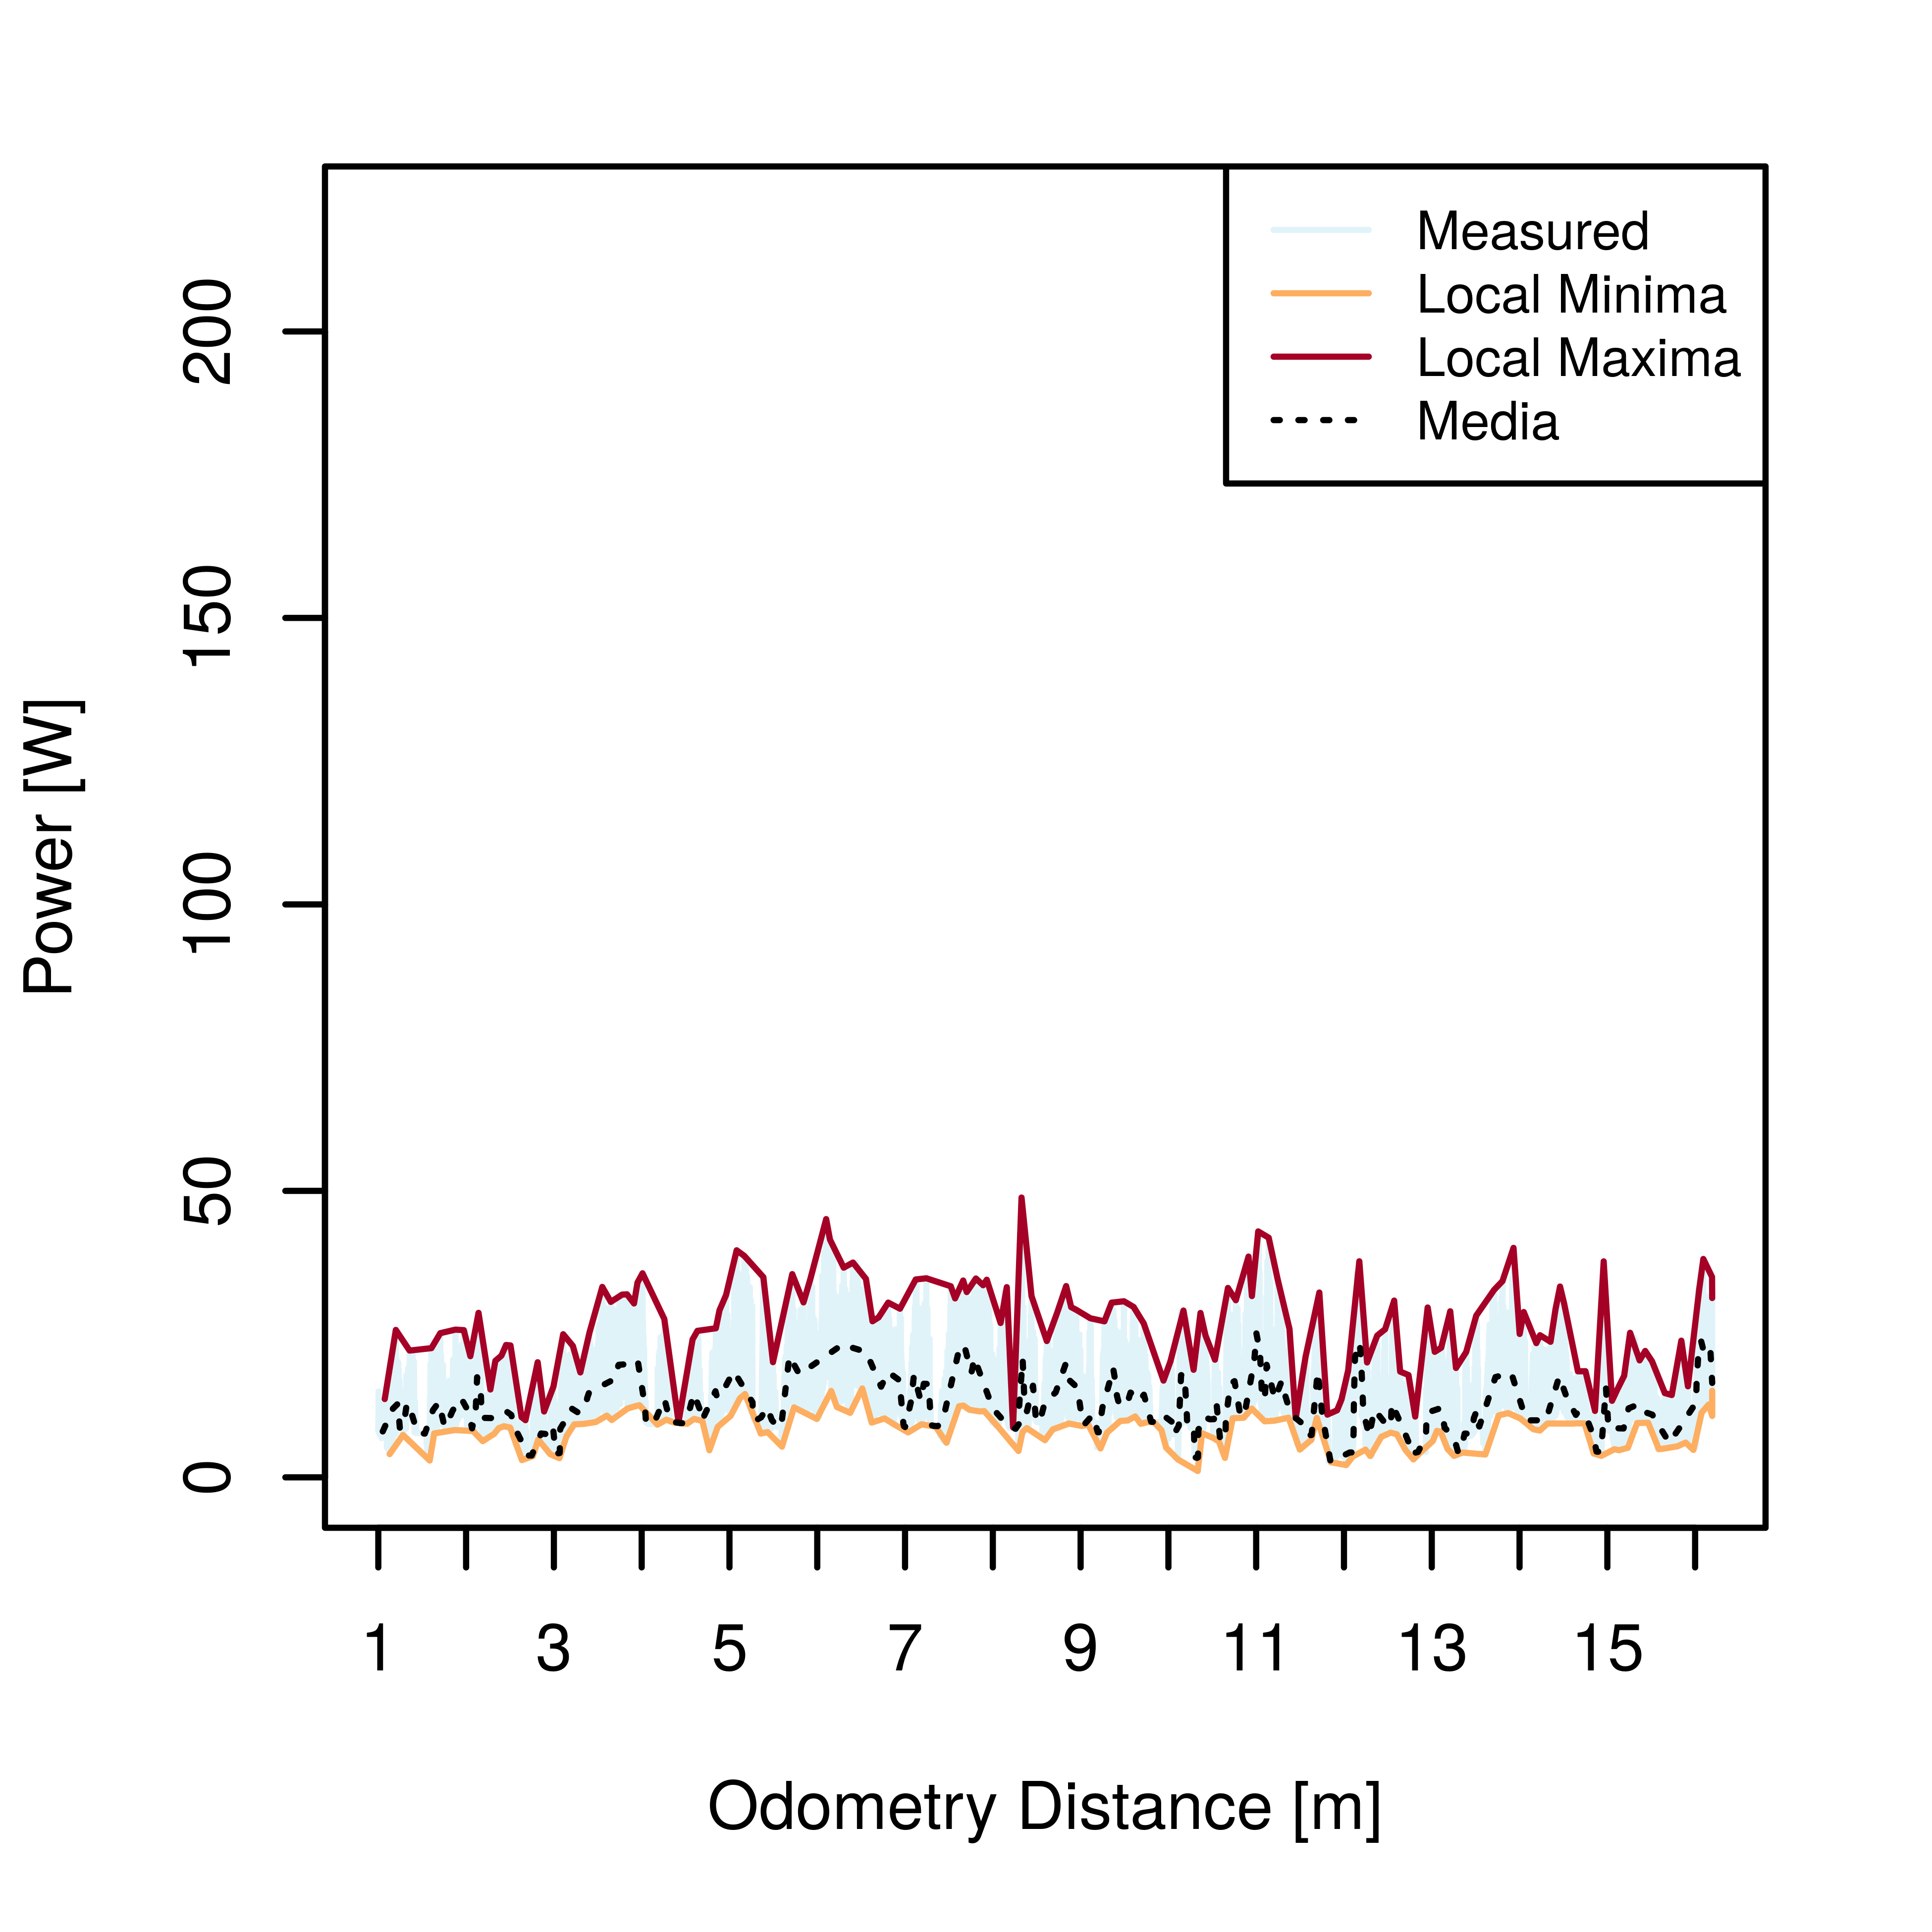
\includegraphics[height=\graphicsHeight]{sections/locomotion-power-draws/plots/suspension-power-draw-on-upslope-terrain.png}
  		\subcaption{Suspension}
		\label{fig:plot:sub:sherpatt-disaggregated-upslope-terrain-power-draw-suspension}
	\end{subfigure}\\[0.8ex]
    \caption[Disaggregated measurements of power draw for upslope terrain traverse during SherpaTT Mars analogue field tests in Utah]
            {Disaggregated measurements of power draw for upslope terrain traverse during SherpaTT Mars analogue field tests in Utah.}
    \label{fig:plot:sherpatt-disaggregated-upslope-terrain-power-draw}
\vspace{-2ex}
\end{figure}

An uplsope traverse has no discernable effect on the suspension power draw, however; there is a clear gradual increase in the drive power draw. The global maximum, minimum, and medium of the traced local minima, maxima, and media power draw lines are presented in Table \ref{tab:sherpatt-upslope-terrain-global-minimum-maximum-and-medium-power-draws}.

\clearpage
\begin{table}[h]
\centering
\caption{Global minimum, maximum, and medium of traced local minima, maxima, and media for SherpaTT upslope terrain traverse propulsion power draw lines.}
\label{tab:sherpatt-upslope-terrain-global-minimum-maximum-and-medium-power-draws}
\begin{tabular}{l|c|c|c|}
\cline{2-4}
\multicolumn{1}{c|}{\multirow{2}{*}{\textbf{}}} & \multicolumn{3}{c|}{\textbf{Power Draw {[}W{]}}} \\ \cline{2-4}
\multicolumn{1}{c|}{} & \textbf{\begin{tabular}[c]{@{}c@{}}Global Minimum\end{tabular}} & \textbf{\begin{tabular}[c]{@{}c@{}}Global Maximum\end{tabular}} & \textbf{\begin{tabular}[c]{@{}c@{}}Global Media\end{tabular}} \\ \hline
\multicolumn{1}{|l|}{\textbf{Measured}} & 34 & 218 & 114 \\ \hline
\multicolumn{1}{|l|}{\textbf{Local Minima}} & 34 & 172 & 98 \\ \hline
\multicolumn{1}{|l|}{\textbf{Local Maxima}} & 54 & 218 & 133 \\ \hline
\multicolumn{1}{|l|}{\textbf{Local Media}} & 40 & 188 & 18 \\ \hline
\end{tabular}
\end{table}


Figure \ref{fig:plot:sherpatt-upslope-terrain-power-draw} overlaps the propulsion local media power draws with the tackled slope angles. The steepest slope angle was \SI{28}{\degree} for an average of \SI{17.52}{\degree}. Slope angle increase are consistently followed by power draw spikes, i.e. at approximately 3, 4, 5, 6, 8, and 9 meters in the odometry measurements. Inversely, slope angle decreases were followed by power draws troughs at approximately 11, 13, 14, and 16 meters.

\begin{figure}[h]
  \centering
  \hypersetup{linkcolor=captionTextColor}
  \includegraphics[width=0.8\linewidth]{sections/locomotion-power-draws/plots/minima-locomotion-power-draws-on-upslope-terrain.png}\\
  \caption[Mean Propulsion power draw for an upslope terrain traverse during SherpaTT Utah field test campaign.]
          {Mean Propulsion power draw for an upslope terrain traverse during SherpaTT Utah field test campaign.}
  \label{fig:plot:sherpatt-upslope-terrain-power-draw}
\end{figure}

The power draws trough following the slope angle change from \SI{28}{\degree} to \SI{20}{\degree} at the \SI{11}{\meter} mark is subsequently followed by an unusual power draw increase and fluctuation. These measurements were discarded as they are outliers with respect to the power draw responses for the slope angle descreases that followed.

Table \ref{tab:sherpatt-upslope-terrain-local-media-measurement-summary} summarises the minimum, maximum, and mean local media propulsion power draws that were measured for different slope angles. Discarding the outlier measurements subsequent to the slope angle change from \SI{28}{\degree} to \SI{20}{\degree} at the \SI{11}{\meter} to \SI{13}{\meter} portion of the track, the maximum mean local media propulsion power draw is \SI{146}{\watt}.

\clearpage
\begin{table}[h]
\centering
\caption{SherpaTT mean propulsion power draw measurements for different slope sections}
\label{tab:sherpatt-upslope-terrain-local-media-measurement-summary}
\begin{tabular}{cc|c|c|c|}
\cline{3-5}
\multicolumn{1}{l}{} & \multicolumn{1}{l|}{} & \multicolumn{3}{c|}{\textbf{Power {[}W{]}}} \\ \hline
\multicolumn{1}{|l|}{\textbf{Distance {[}m{]}}} & \multicolumn{1}{l|}{\textbf{Slope Angle {[}deg{]}}} & \multicolumn{1}{l|}{\textbf{Minimum}} & \multicolumn{1}{l|}{\textbf{Maximum}} & \multicolumn{1}{l|}{\textbf{Mean}} \\ \hline
\multicolumn{1}{|c|}{\textbf{1 $<$ x $\leq$ 3}} & 10 & 40 & 64 & 51 \\ \hline
\multicolumn{1}{|c|}{\textbf{3 $<$ x $\leq$ 4}} & 11 & 73 & 93 & 85 \\ \hline
\multicolumn{1}{|c|}{\textbf{4 $<$ x $\leq$ 5}} & 15 & 74 & 87 & 83 \\ \hline
\multicolumn{1}{|c|}{\textbf{5 $<$ x $\leq$ 6}} & 16 & 85 & 125 & 107 \\ \hline
\multicolumn{1}{|c|}{\textbf{6 $<$ x $\leq$ 7}} & 28 & 98 & 141 & 123 \\ \hline
\multicolumn{1}{|c|}{\textbf{7 $<$ x $\leq$ 8}} & 22 & 97 & 139 & 116 \\ \hline
\multicolumn{1}{|c|}{\textbf{8 $<$ x $\leq$ 9}} & 25 & 113 & 164 & 133 \\ \hline
\multicolumn{1}{|c|}{\textbf{9 $<$ x $\leq$ 11}} & 28 & 114 & 176 & 146 \\ \hline
\multicolumn{1}{|c|}{\textbf{11 $<$ x $\leq$ 13}} & 20 & 135 & 188 & 167 \\ \hline
\multicolumn{1}{|c|}{\textbf{13 $<$ x $\leq$ 14}} & 15 & 119 & 123 & 145 \\ \hline
\multicolumn{1}{|c|}{\textbf{14 $<$ x $\leq$ 16}} & 10 & 70 & 186 & 94 \\ \hline
\end{tabular}
\end{table}


\section{Conclusion}
\label{sec:PropulsionPowerConstraints:Conclusion}
Based on data from the SherpaTT field campaign and the assumptions made in Section \ref{sec:PropulsionPowerConstraints:Introduction}, the following power subsystem requirements were proposed with respect to propulsion power draws:

\begin{itemize}
    \item The rover shall provide up to \SI{75}{\watt} in propulsion power for flat terrain traverses.
    \item The rover shall provide up to \SI{150}{\watt} in propulsion power for upslope terrain traverses of up to \SI{30}{\degree} inclination.
\end{itemize}


\clearpage
\section{Simulation}
\label{sec:Design:Simulation}
\section{Introduction}
\label{sec:PropulsionPowerConstraints:Introduction}
SherpaTT's actively articulated suspension system consists of 4 wheeled-legs with a total of 20 motors. Each leg is equipped with 3 suspension motors and 2 drive motors. The suspension motors are responsible for Pan, \ac{IL}, and \ac{OL} revolute joint rotations whereas the drive motors are responsible for \ac{WS} and \ac{WD}. The distribution of these motors across each leg are shown in Figure \ref{fig:sherpatt-actively-articulated-suspension-system}. Propulsion power draw refers to the summation of suspension and drive motor power draws. These power draws have been studied in detail for SherpaTT during a Mars analogue field campaign in Utah \citeother{Cordes2018}.

\begin{figure}[h]
  \centering
  \hypersetup{linkcolor=captionTextColor}
  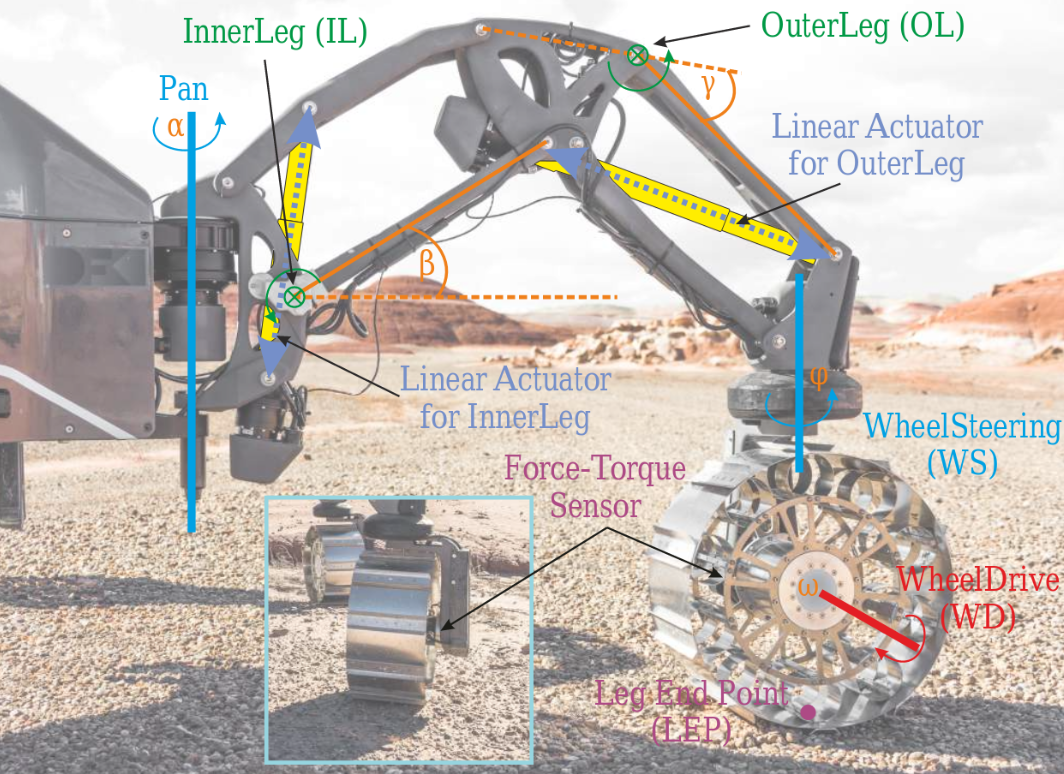
\includegraphics[width=0.8\linewidth]{sections/locomotion-power-draws/images/sherpatt-actively-articulated-suspension-sytem.png}\\
  \caption[SherpaTT actively articulated suspension system]
          {SherpaTT actively articulated suspension system.}
  \label{fig:sherpatt-actively-articulated-suspension-system}
\end{figure}

 This section restricts power draw analysis to establishing propulsion power constraints for the study of SherpaTT Mars mission scenarios. Lack of motor optimisation as well as lower gravity and pressure on Mars permit the assumption that, given similar topology traversals, measured propulsion power draws are greater than those that would be observed on a Martian environment. This assumption is further supported when considering that SherpaTT's velocities during power draw measurements were much greater than what has been achieved on present and past Mars rover missions.


\section{Power Draw}
\label{sec:PropulsionPowerConstraints:PowerDraw}
Available datasets from the Mars analogue field test campaign cover 2 flat surface runs and 3 steep upslope terrain runs. From the 2 upslope runs, the dataset with the worst-case maximum and mean propulsion power draw was used as the worst-case scenario. Hereafter, all mention of SherpaTT power draws will reference measurements included in these datasets. Measured power draws fluctuate due to slips, skids, noise, and other unknown imperfections. To ease readability, local minima, maxima, and media lines have been traced for all power plot figures.


\subsection{Flat Terrain Traverse}
\label{sec:PropulsionPowerConstraints:FlatTerrainTraverse}
\ac{MER} and \ac{MSL} rovers are each equipped with a total of 10 propulsion motors to drive their Rocker-Bogie passive suspension system: 6 to rotate the wheels and 4 to steer them \citeother{Novak2005} \citeother{Lakdawalla2018}. The \ac{MER} rovers needed approximately \SI{100}{\watt} to drive \citeother{MERRoverEnergy}. Propulsion power draws measured for SherpaTT on flat surface runs are shown in Figure \ref{fig:plot:sherpatt-flat-terrain-power-draw}.

\begin{figure}[h]
\captionsetup[subfigure]{justification=centering}
\vspace{-2ex}
	\centering
    %% setup sizes
    \setlength{\subfigureWidth}{0.50\textwidth}
    \setlength{\graphicsHeight}{80mm}
    %% kill hyper-link highlighting
    \hypersetup{hidelinks=true}%
    %% the figures
    \begin{subfigure}[t]{\subfigureWidth}
        \centering
        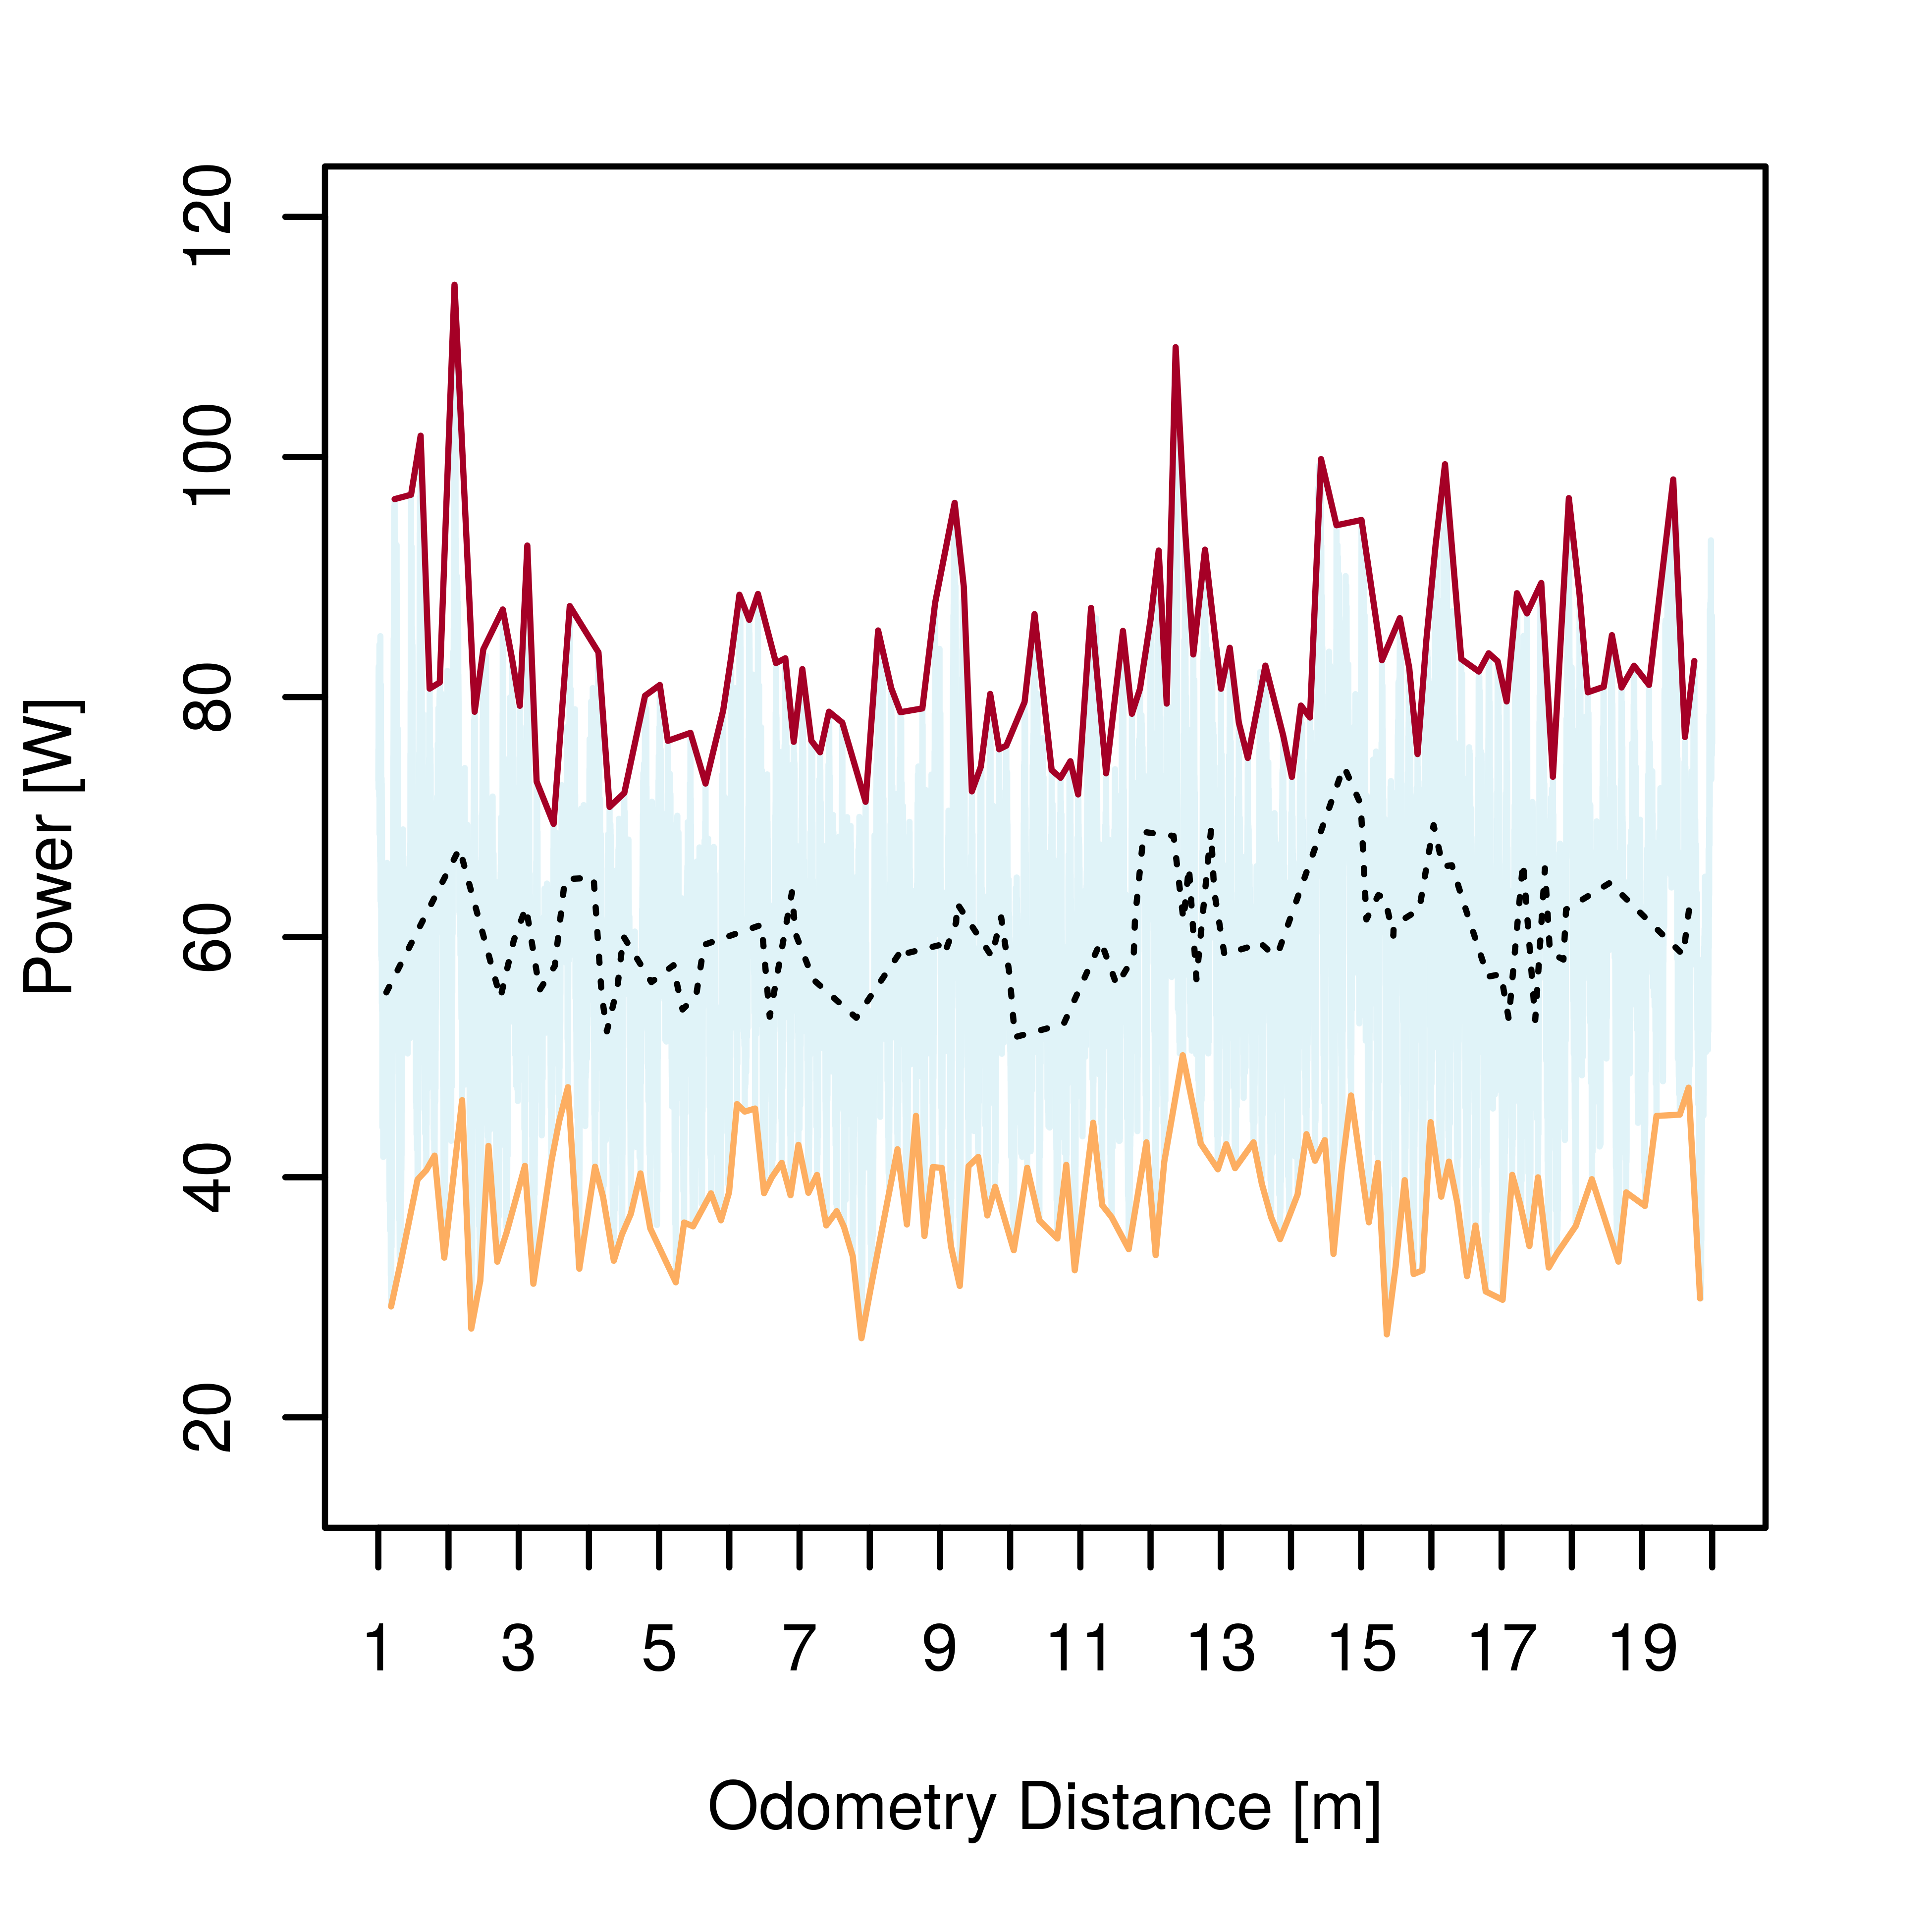
\includegraphics[height=\graphicsHeight]{sections/locomotion-power-draws/plots/locomotion-power-draw-on-flat-terrain-1.png}
        \subcaption{Run \#1}
        \label{fig:plot:sub:sherpatt-flat-terrain-power-draw-1}
    \end{subfigure}\hfill
    \begin{subfigure}[t]{\subfigureWidth}
        \centering
        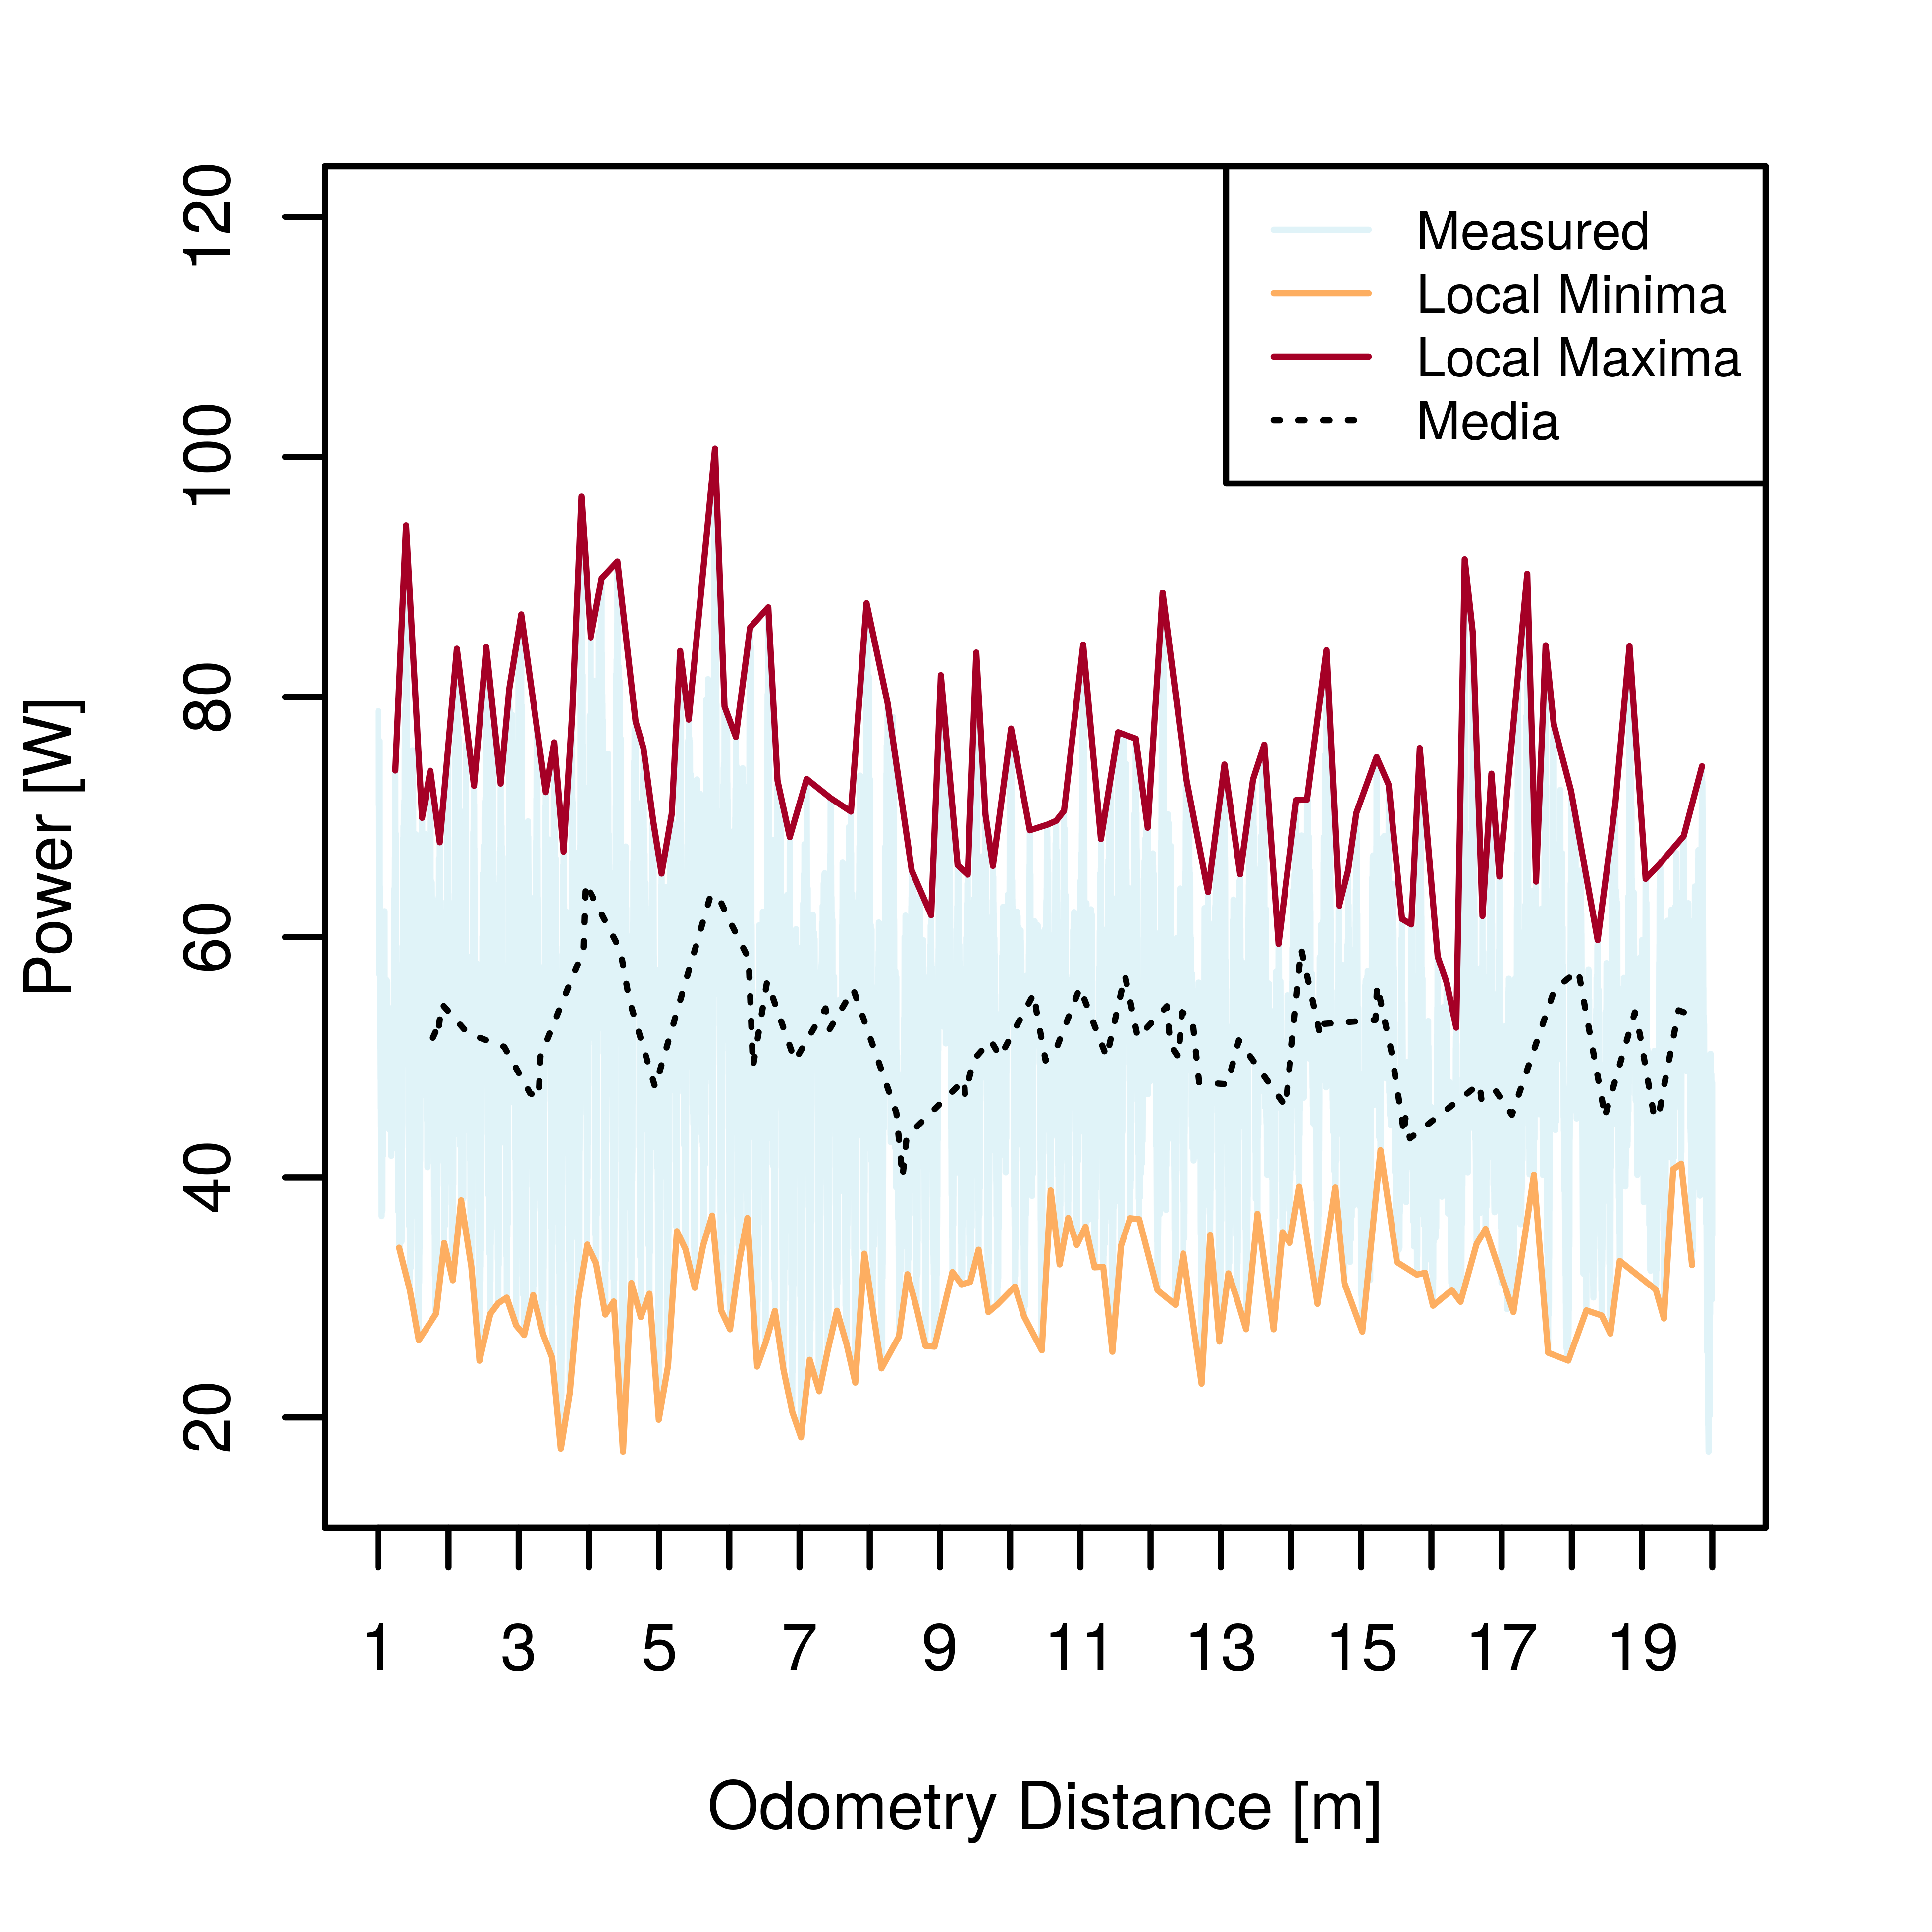
\includegraphics[height=\graphicsHeight]{sections/locomotion-power-draws/plots/locomotion-power-draw-on-flat-terrain-2.png}
  		\subcaption{Run \#2}
		\label{fig:plot:sub:sherpatt-flat-terrain-power-draw-2}
	\end{subfigure}\\[0.8ex]
    \caption[Propulsion power draw for a flat terrain traverse during SherpaTT Mars analogue field tests in Utah]
            {Propulsion power draw for a flat terrain traverse during SherpaTT Mars analogue field tests in Utah.}
    \label{fig:plot:sherpatt-flat-terrain-power-draw}
\vspace{-2ex}
\end{figure}


These measurements are summarised in Table \ref{tab:sherpatt-flat-terrain-global-minimum-maximum-and-medium-power-draws}. To eliminate power draw fluctuations from the analysis, only local media values were considered. Local media were selected rather than the worst-case local maxima on the basis of the assumptions made in Section \ref{sec:PropulsionPowerConstraints:Introduction}. For flat terrain traverses, a worst-case maximum power draw of \SI{74}{\watt} is observed for a mean of \SI{61}{\watt}.

\clearpage
\begin{table}[h]
\centering
\caption{Global minimum, maximum, and medium of traced local minima, maxima, and media for SherpaTT flat terrain propulsion power draw lines.}
\label{tab:sherpatt-flat-terrain-global-minimum-maximum-and-medium-power-draws}
\begin{tabular}{llccc}
\cline{3-5}
\multicolumn{2}{l|}{\multirow{2}{*}{}} & \multicolumn{3}{c|}{\textbf{Power Draw {[}W{]}}} \\ \cline{3-5}
\multicolumn{2}{l|}{} & \multicolumn{1}{c|}{\textbf{\begin{tabular}[c]{@{}c@{}}Global Minimum\end{tabular}}} & \multicolumn{1}{c|}{\textbf{\begin{tabular}[c]{@{}c@{}}Global Maximum\end{tabular}}} & \multicolumn{1}{c|}{\textbf{\begin{tabular}[c]{@{}c@{}}Global Media\end{tabular}}} \\ \hline
\multicolumn{1}{|c|}{\multirow{4}{*}{\textbf{Run \#1}}} & \multicolumn{1}{l|}{\textbf{Measured}} & \multicolumn{1}{c|}{27} & \multicolumn{1}{c|}{114} & \multicolumn{1}{c|}{60} \\ \cline{2-5}
\multicolumn{1}{|c|}{} & \multicolumn{1}{l|}{\textbf{Local Minima}} & \multicolumn{1}{c|}{27} & \multicolumn{1}{c|}{50} & \multicolumn{1}{c|}{38} \\ \cline{2-5}
\multicolumn{1}{|c|}{} & \multicolumn{1}{l|}{\textbf{Local Maxima}} & \multicolumn{1}{c|}{69} & \multicolumn{1}{c|}{114} & \multicolumn{1}{c|}{83} \\ \cline{2-5}
\multicolumn{1}{|c|}{} & \multicolumn{1}{l|}{\textbf{Local Media}} & \multicolumn{1}{c|}{52} & \multicolumn{1}{c|}{74} & \multicolumn{1}{c|}{61} \\ \hhline{|=|=|=|=|=|}
\multicolumn{1}{|l|}{\multirow{4}{*}{\textbf{Run \#2}}} & \multicolumn{1}{l|}{\textbf{Measured}} & \multicolumn{1}{c|}{17} & \multicolumn{1}{c|}{101} & \multicolumn{1}{c|}{51} \\ \cline{2-5}
\multicolumn{1}{|l|}{} & \multicolumn{1}{l|}{\textbf{Local Minima}} & \multicolumn{1}{c|}{17} & \multicolumn{1}{c|}{42} & \multicolumn{1}{c|}{30} \\ \cline{2-5}
\multicolumn{1}{|l|}{} & \multicolumn{1}{l|}{\textbf{Local Maxima}} & \multicolumn{1}{c|}{52} & \multicolumn{1}{c|}{101} & \multicolumn{1}{c|}{74} \\ \cline{2-5}
\multicolumn{1}{|l|}{} & \multicolumn{1}{l|}{\textbf{Local Media}} & \multicolumn{1}{c|}{40} & \multicolumn{1}{c|}{64} & \multicolumn{1}{c|}{52} \\ \hline
 &  & \multicolumn{1}{l}{} & \multicolumn{1}{l}{} & \multicolumn{1}{l}{} \\
 &  & \multicolumn{1}{l}{} & \multicolumn{1}{l}{} & \multicolumn{1}{l}{}
\end{tabular}
\end{table}


\subsection{Upslope Terrain Traverse}
\label{sec:PropulsionPowerConstraints:UpslopeTerrainTraverse}
Propulsion power draws on a steep uplsope were measured along an approximately \SI{16}{\meter} track and are shown Figure \ref{fig:plot:sub:sherpatt-disaggregated-upslope-terrain-power-draw-locomotion}. The drive and suspension power draw components are shown in Figures \ref{fig:plot:sub:sherpatt-disaggregated-upslope-terrain-power-draw-drive} and \ref{fig:plot:sub:sherpatt-disaggregated-upslope-terrain-power-draw-suspension}, respectively.

\begin{figure}[h]
\captionsetup[subfigure]{justification=centering}
\vspace{-2ex}
	\centering
    %% setup sizes
    \setlength{\subfigureWidth}{0.32\textwidth}
    \setlength{\graphicsHeight}{50mm}
    %% kill hyper-link highlighting
    \hypersetup{hidelinks=true}%
    %% the figures
	\begin{subfigure}[t]{\subfigureWidth}
        \centering
        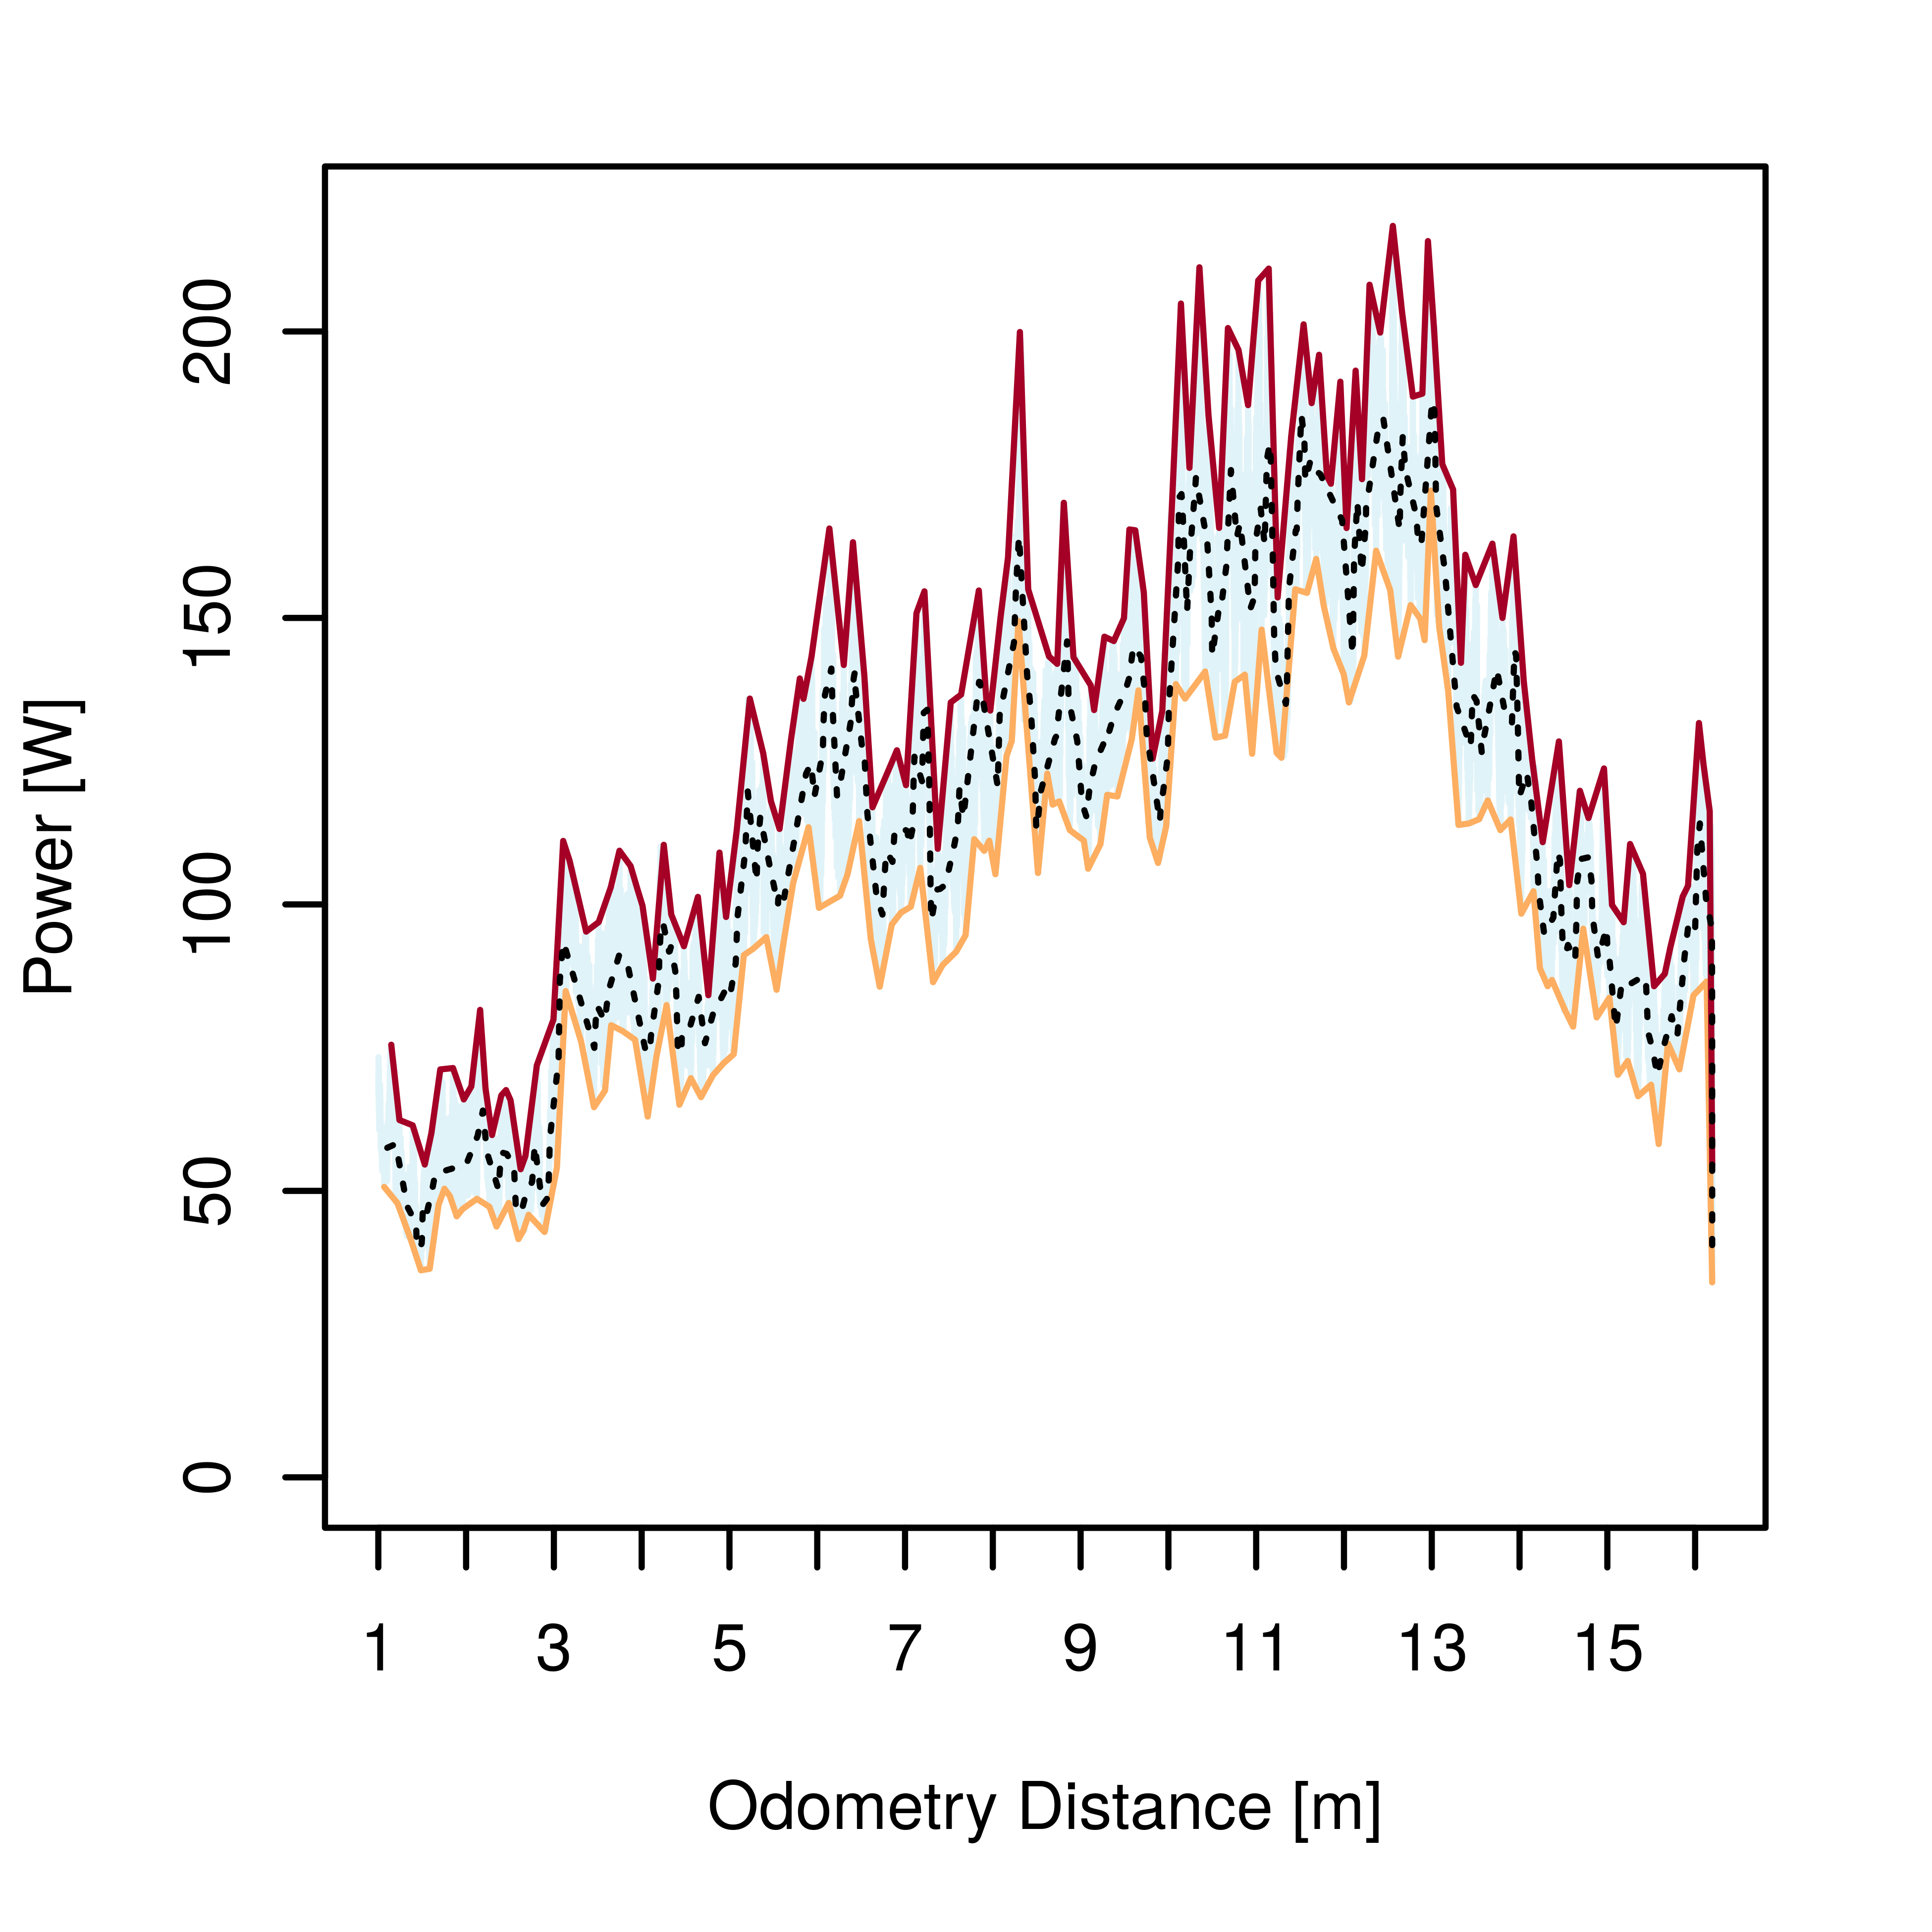
\includegraphics[height=\graphicsHeight]{sections/locomotion-power-draws/plots/locomotion-power-draw-on-upslope-terrain.png}
  		\subcaption{Propulsion}
		\label{fig:plot:sub:sherpatt-disaggregated-upslope-terrain-power-draw-locomotion}
	\end{subfigure}\hfill
	\begin{subfigure}[t]{\subfigureWidth}
        \centering
        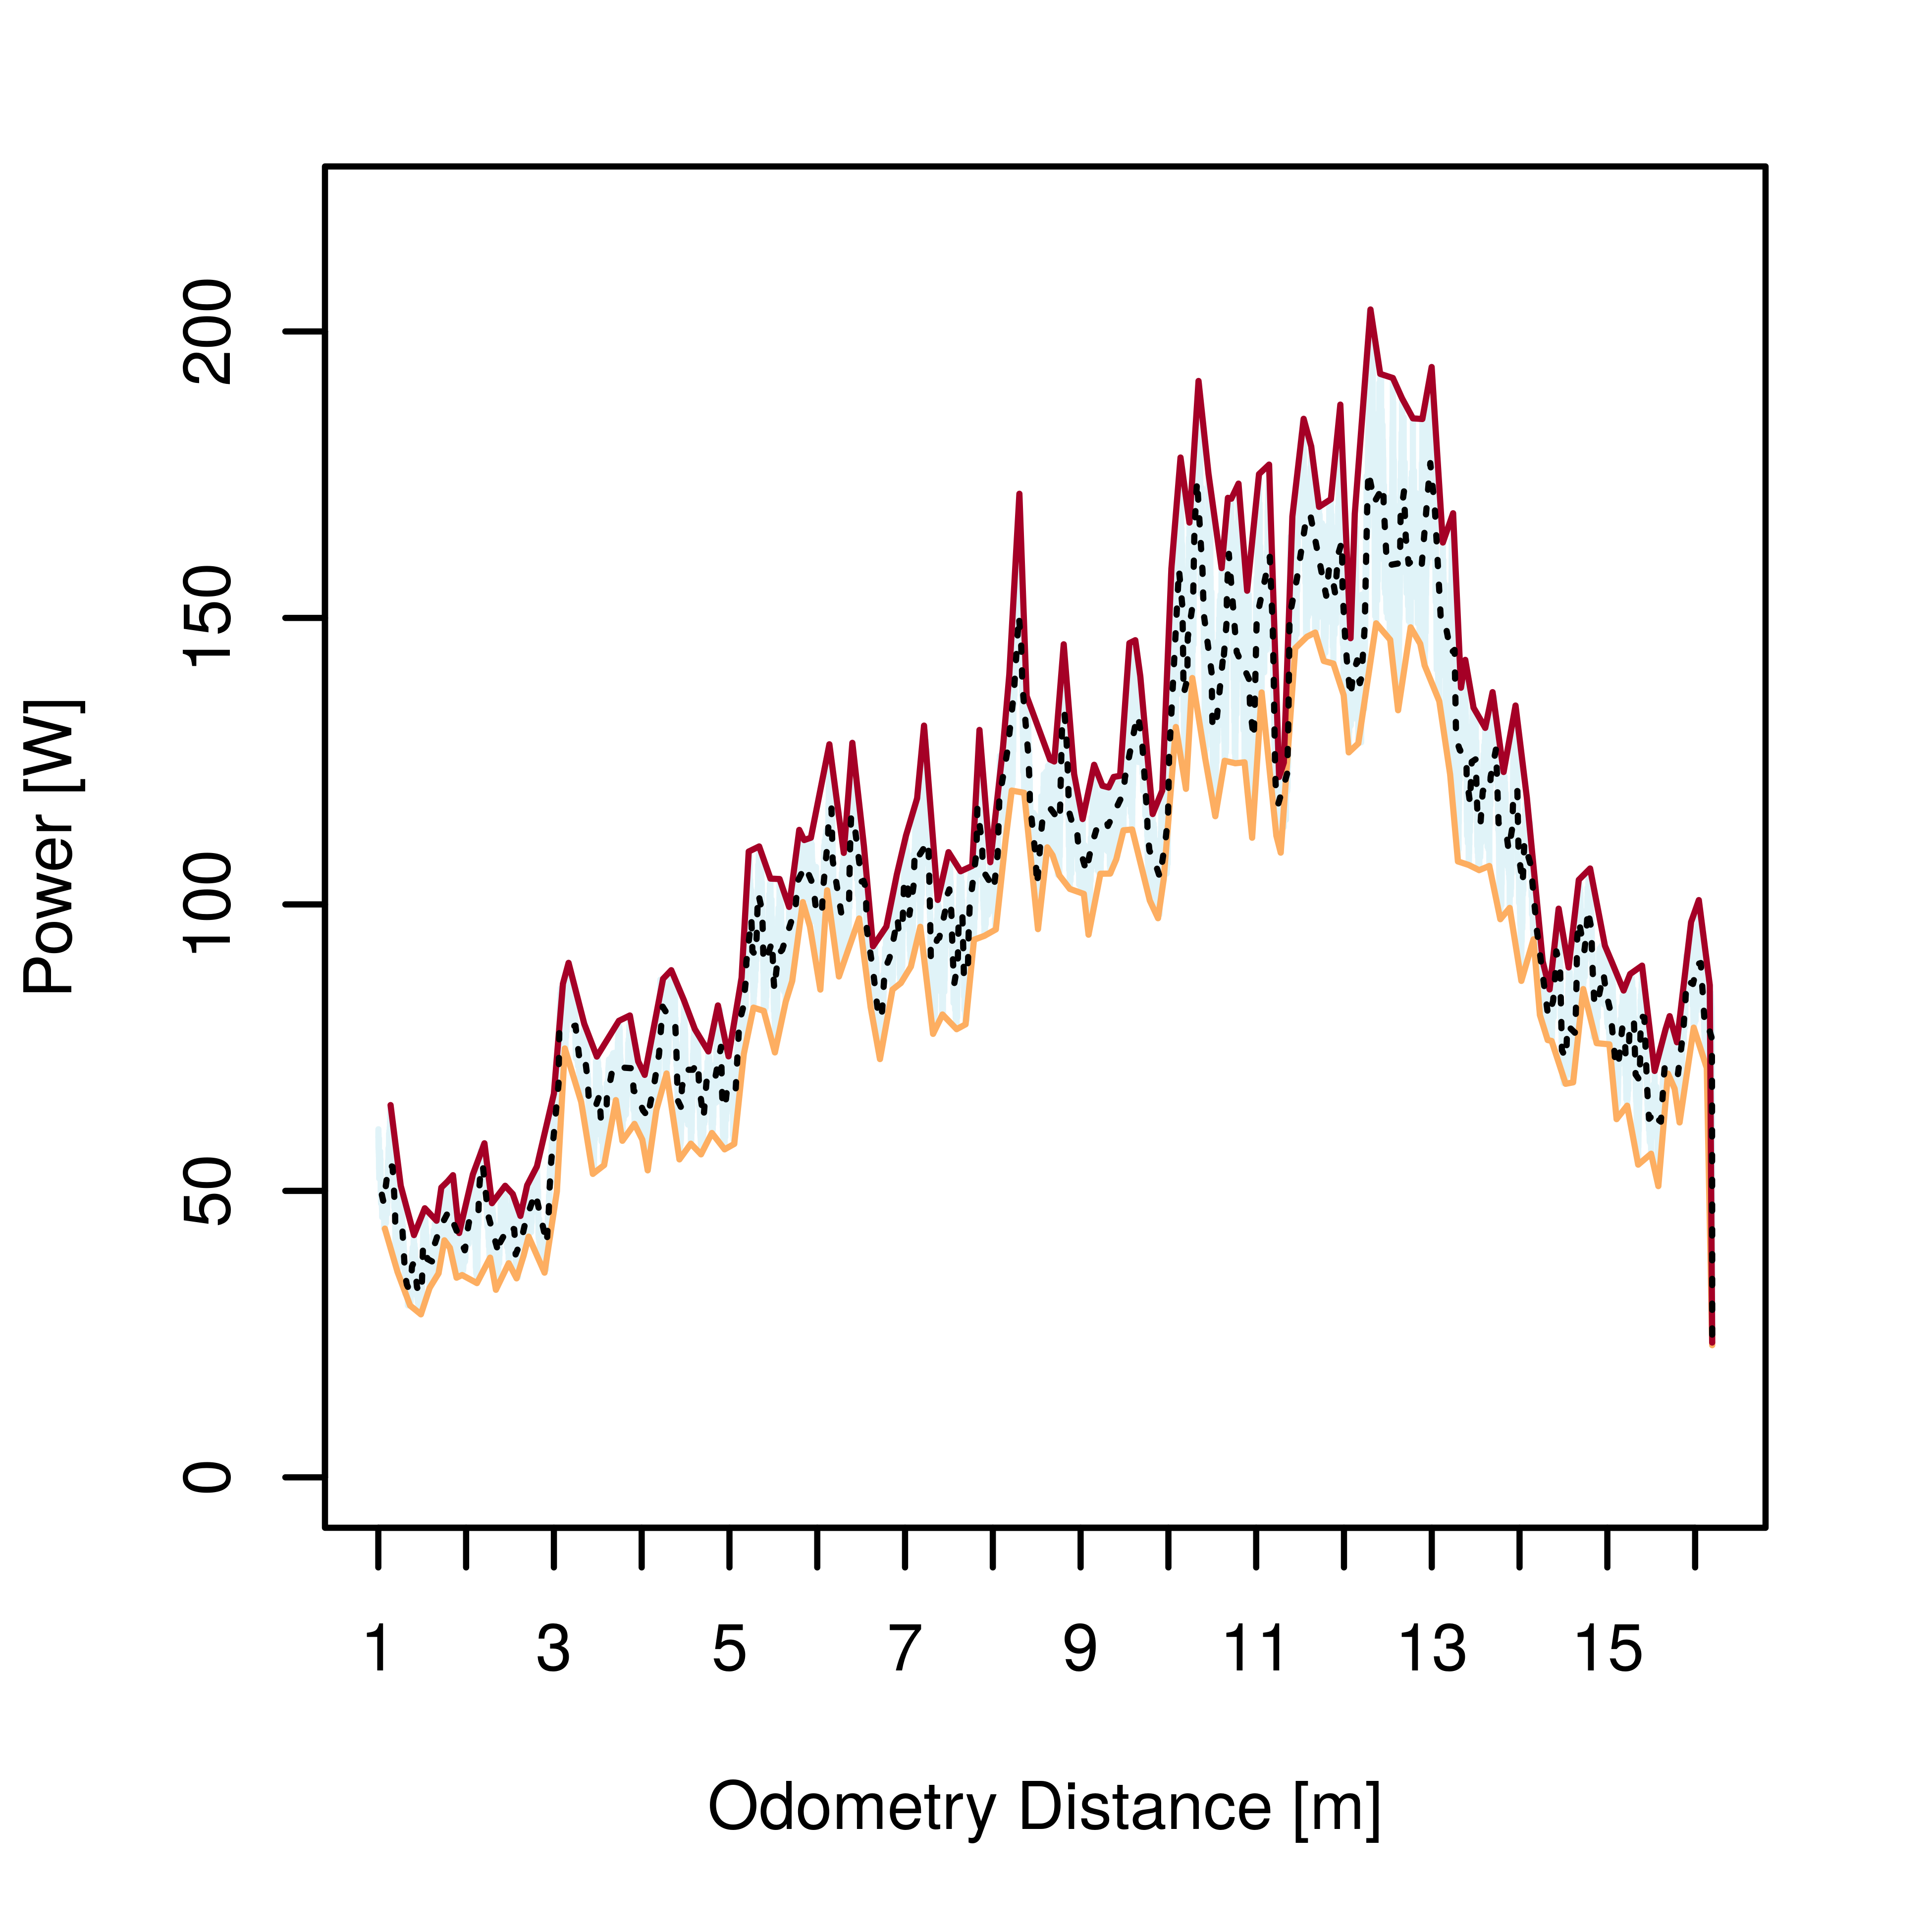
\includegraphics[height=\graphicsHeight]{sections/locomotion-power-draws/plots/drive-power-draw-on-upslope-terrain.png}
  		\subcaption{Drive}
		\label{fig:plot:sub:sherpatt-disaggregated-upslope-terrain-power-draw-drive}
	\end{subfigure}\hfill
    \begin{subfigure}[t]{\subfigureWidth}
        \centering
        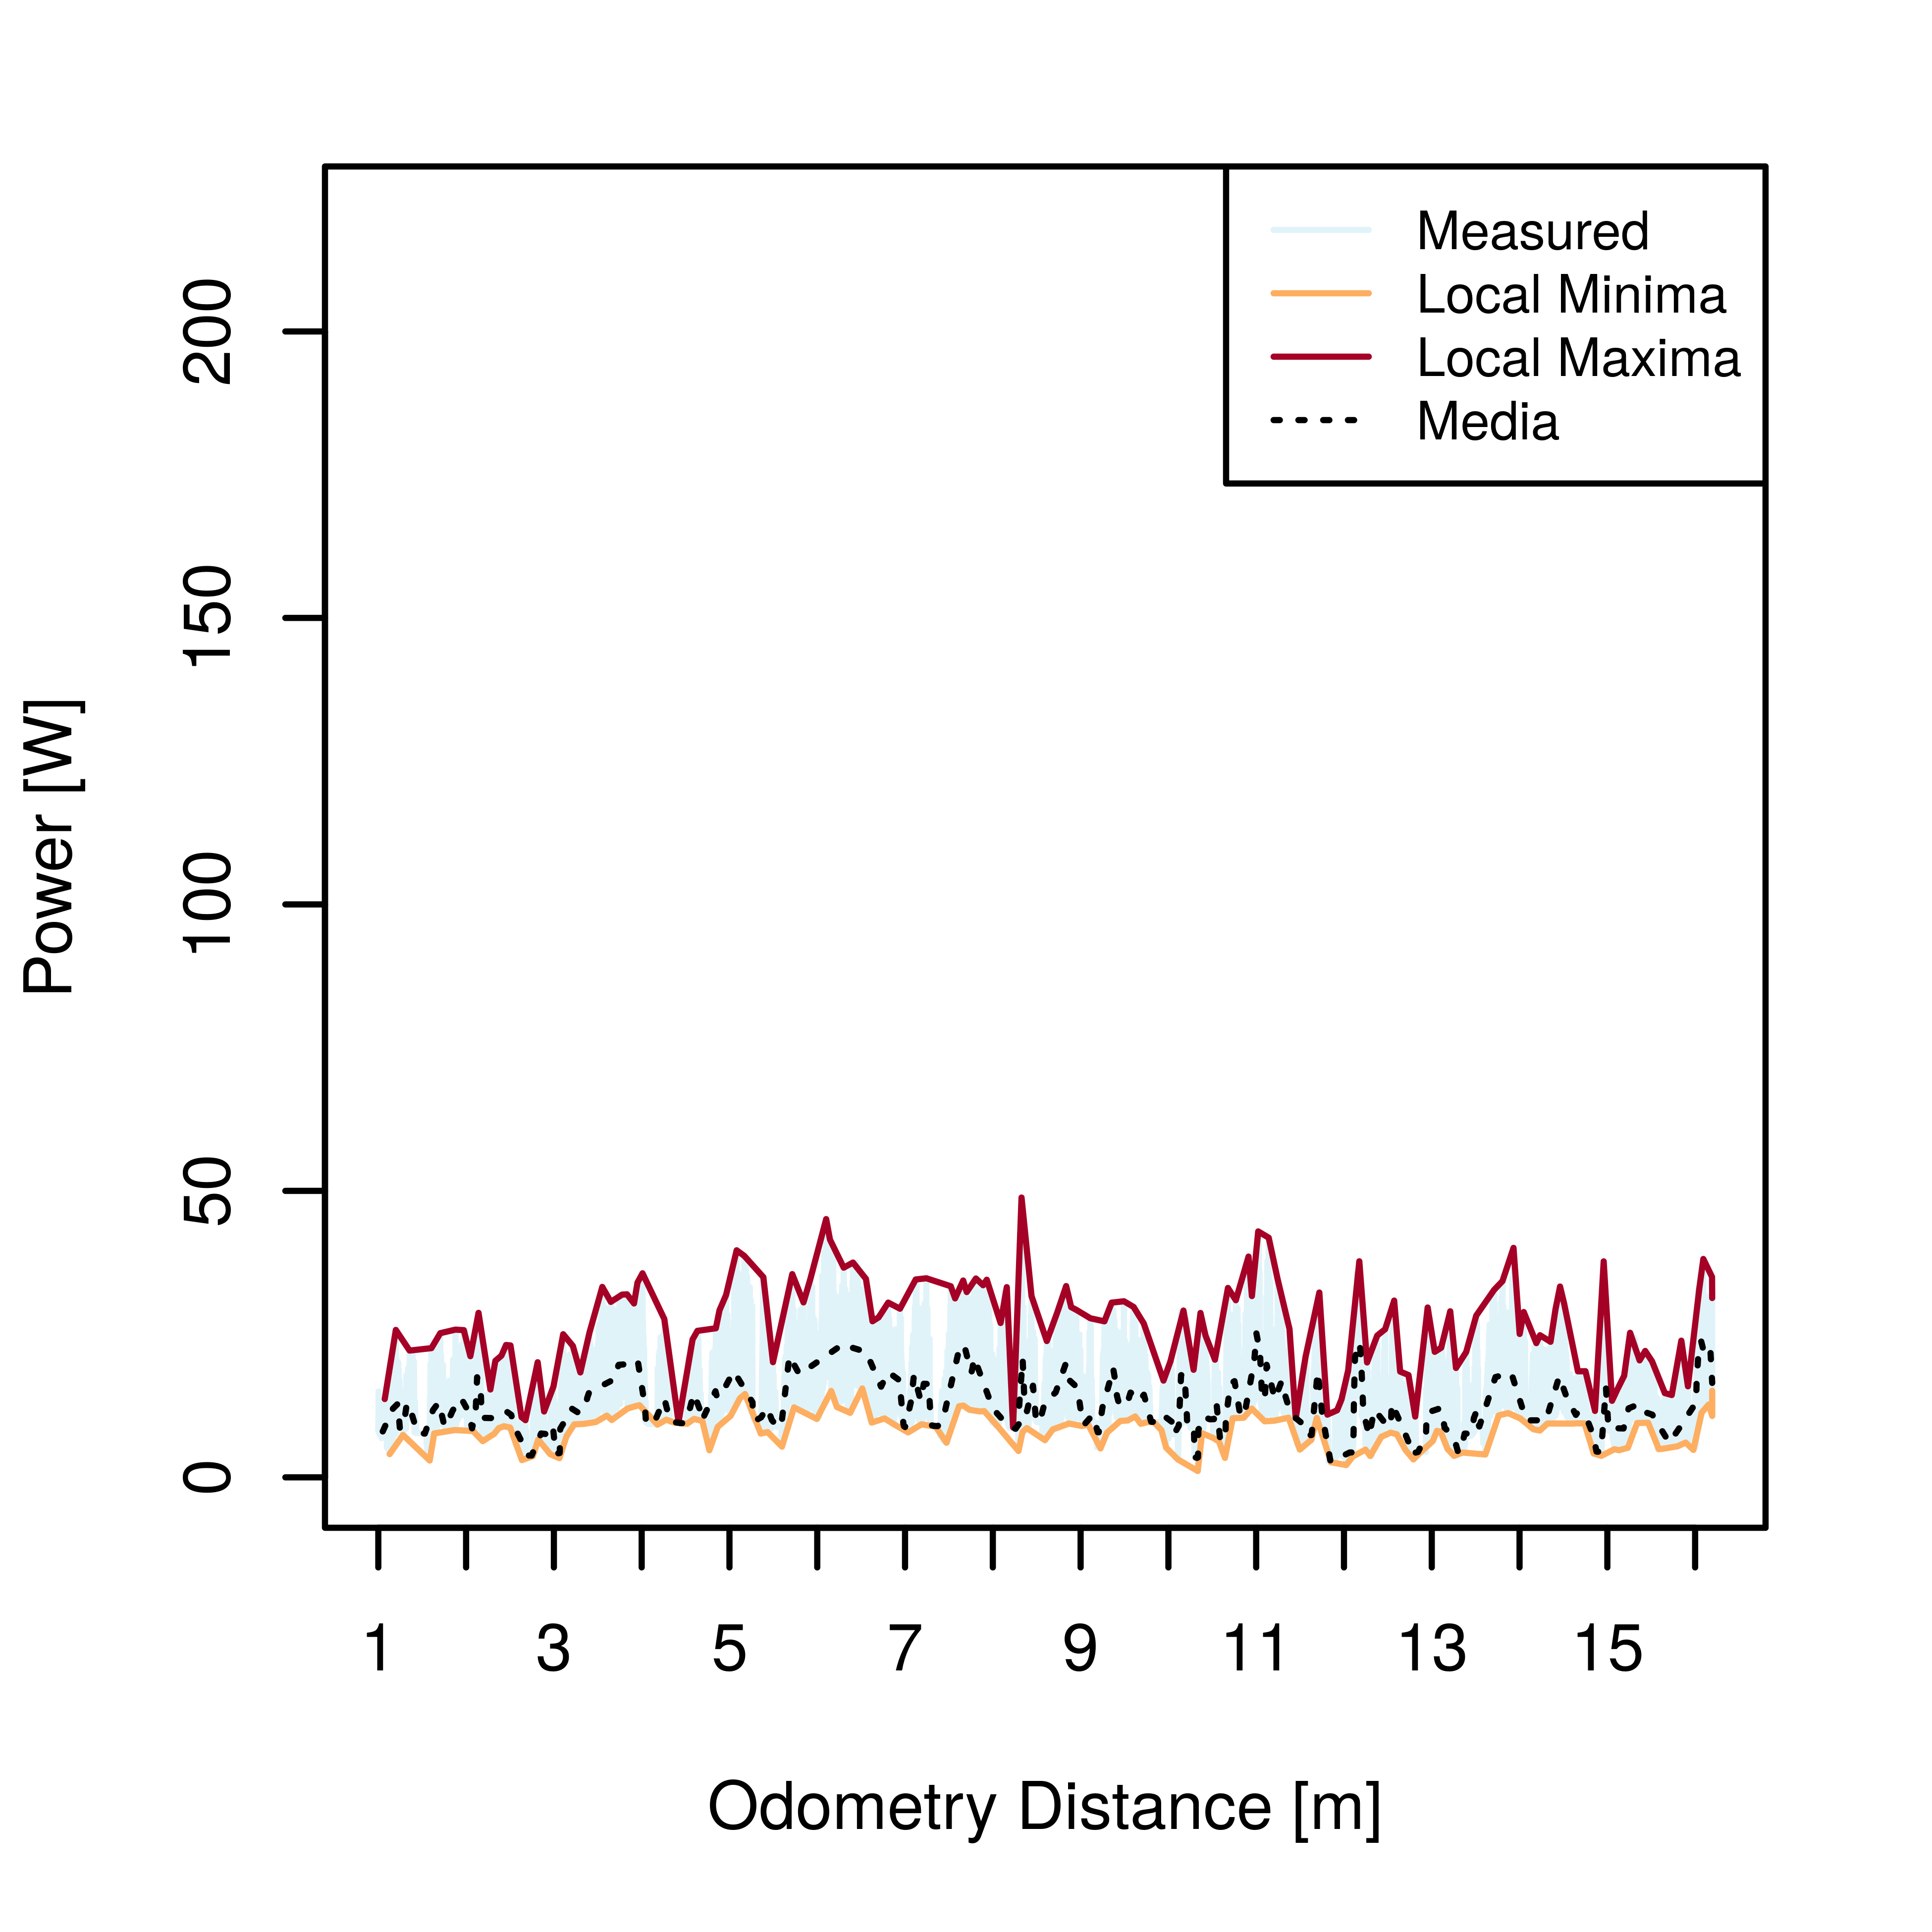
\includegraphics[height=\graphicsHeight]{sections/locomotion-power-draws/plots/suspension-power-draw-on-upslope-terrain.png}
  		\subcaption{Suspension}
		\label{fig:plot:sub:sherpatt-disaggregated-upslope-terrain-power-draw-suspension}
	\end{subfigure}\\[0.8ex]
    \caption[Disaggregated measurements of power draw for upslope terrain traverse during SherpaTT Mars analogue field tests in Utah]
            {Disaggregated measurements of power draw for upslope terrain traverse during SherpaTT Mars analogue field tests in Utah.}
    \label{fig:plot:sherpatt-disaggregated-upslope-terrain-power-draw}
\vspace{-2ex}
\end{figure}

An uplsope traverse has no discernable effect on the suspension power draw, however; there is a clear gradual increase in the drive power draw. The global maximum, minimum, and medium of the traced local minima, maxima, and media power draw lines are presented in Table \ref{tab:sherpatt-upslope-terrain-global-minimum-maximum-and-medium-power-draws}.

\clearpage
\begin{table}[h]
\centering
\caption{Global minimum, maximum, and medium of traced local minima, maxima, and media for SherpaTT upslope terrain traverse propulsion power draw lines.}
\label{tab:sherpatt-upslope-terrain-global-minimum-maximum-and-medium-power-draws}
\begin{tabular}{l|c|c|c|}
\cline{2-4}
\multicolumn{1}{c|}{\multirow{2}{*}{\textbf{}}} & \multicolumn{3}{c|}{\textbf{Power Draw {[}W{]}}} \\ \cline{2-4}
\multicolumn{1}{c|}{} & \textbf{\begin{tabular}[c]{@{}c@{}}Global Minimum\end{tabular}} & \textbf{\begin{tabular}[c]{@{}c@{}}Global Maximum\end{tabular}} & \textbf{\begin{tabular}[c]{@{}c@{}}Global Media\end{tabular}} \\ \hline
\multicolumn{1}{|l|}{\textbf{Measured}} & 34 & 218 & 114 \\ \hline
\multicolumn{1}{|l|}{\textbf{Local Minima}} & 34 & 172 & 98 \\ \hline
\multicolumn{1}{|l|}{\textbf{Local Maxima}} & 54 & 218 & 133 \\ \hline
\multicolumn{1}{|l|}{\textbf{Local Media}} & 40 & 188 & 18 \\ \hline
\end{tabular}
\end{table}


Figure \ref{fig:plot:sherpatt-upslope-terrain-power-draw} overlaps the propulsion local media power draws with the tackled slope angles. The steepest slope angle was \SI{28}{\degree} for an average of \SI{17.52}{\degree}. Slope angle increase are consistently followed by power draw spikes, i.e. at approximately 3, 4, 5, 6, 8, and 9 meters in the odometry measurements. Inversely, slope angle decreases were followed by power draws troughs at approximately 11, 13, 14, and 16 meters.

\begin{figure}[h]
  \centering
  \hypersetup{linkcolor=captionTextColor}
  \includegraphics[width=0.8\linewidth]{sections/locomotion-power-draws/plots/minima-locomotion-power-draws-on-upslope-terrain.png}\\
  \caption[Mean Propulsion power draw for an upslope terrain traverse during SherpaTT Utah field test campaign.]
          {Mean Propulsion power draw for an upslope terrain traverse during SherpaTT Utah field test campaign.}
  \label{fig:plot:sherpatt-upslope-terrain-power-draw}
\end{figure}

The power draws trough following the slope angle change from \SI{28}{\degree} to \SI{20}{\degree} at the \SI{11}{\meter} mark is subsequently followed by an unusual power draw increase and fluctuation. These measurements were discarded as they are outliers with respect to the power draw responses for the slope angle descreases that followed.

Table \ref{tab:sherpatt-upslope-terrain-local-media-measurement-summary} summarises the minimum, maximum, and mean local media propulsion power draws that were measured for different slope angles. Discarding the outlier measurements subsequent to the slope angle change from \SI{28}{\degree} to \SI{20}{\degree} at the \SI{11}{\meter} to \SI{13}{\meter} portion of the track, the maximum mean local media propulsion power draw is \SI{146}{\watt}.

\clearpage
\begin{table}[h]
\centering
\caption{SherpaTT mean propulsion power draw measurements for different slope sections}
\label{tab:sherpatt-upslope-terrain-local-media-measurement-summary}
\begin{tabular}{cc|c|c|c|}
\cline{3-5}
\multicolumn{1}{l}{} & \multicolumn{1}{l|}{} & \multicolumn{3}{c|}{\textbf{Power {[}W{]}}} \\ \hline
\multicolumn{1}{|l|}{\textbf{Distance {[}m{]}}} & \multicolumn{1}{l|}{\textbf{Slope Angle {[}deg{]}}} & \multicolumn{1}{l|}{\textbf{Minimum}} & \multicolumn{1}{l|}{\textbf{Maximum}} & \multicolumn{1}{l|}{\textbf{Mean}} \\ \hline
\multicolumn{1}{|c|}{\textbf{1 $<$ x $\leq$ 3}} & 10 & 40 & 64 & 51 \\ \hline
\multicolumn{1}{|c|}{\textbf{3 $<$ x $\leq$ 4}} & 11 & 73 & 93 & 85 \\ \hline
\multicolumn{1}{|c|}{\textbf{4 $<$ x $\leq$ 5}} & 15 & 74 & 87 & 83 \\ \hline
\multicolumn{1}{|c|}{\textbf{5 $<$ x $\leq$ 6}} & 16 & 85 & 125 & 107 \\ \hline
\multicolumn{1}{|c|}{\textbf{6 $<$ x $\leq$ 7}} & 28 & 98 & 141 & 123 \\ \hline
\multicolumn{1}{|c|}{\textbf{7 $<$ x $\leq$ 8}} & 22 & 97 & 139 & 116 \\ \hline
\multicolumn{1}{|c|}{\textbf{8 $<$ x $\leq$ 9}} & 25 & 113 & 164 & 133 \\ \hline
\multicolumn{1}{|c|}{\textbf{9 $<$ x $\leq$ 11}} & 28 & 114 & 176 & 146 \\ \hline
\multicolumn{1}{|c|}{\textbf{11 $<$ x $\leq$ 13}} & 20 & 135 & 188 & 167 \\ \hline
\multicolumn{1}{|c|}{\textbf{13 $<$ x $\leq$ 14}} & 15 & 119 & 123 & 145 \\ \hline
\multicolumn{1}{|c|}{\textbf{14 $<$ x $\leq$ 16}} & 10 & 70 & 186 & 94 \\ \hline
\end{tabular}
\end{table}


\section{Conclusion}
\label{sec:PropulsionPowerConstraints:Conclusion}
Based on data from the SherpaTT field campaign and the assumptions made in Section \ref{sec:PropulsionPowerConstraints:Introduction}, the following power subsystem requirements were proposed with respect to propulsion power draws:

\begin{itemize}
    \item The rover shall provide up to \SI{75}{\watt} in propulsion power for flat terrain traverses.
    \item The rover shall provide up to \SI{150}{\watt} in propulsion power for upslope terrain traverses of up to \SI{30}{\degree} inclination.
\end{itemize}


\section{Summary and Conclusion}
\label{sec:Design:SummaryAndConclusion}
This chapter defines reference Sols and their power budgets from which \ac{SA} design requirements and constraints are fine tuned. Two \ac{SA} designs are proposed, one for each mission site. Their conceptualization is driven by maximizing traverse gains obtained from leveraging the rover's suspension system as a \ac{SA} orientation and inclination mechanism. The results obtained from simulations are described which showcase the solar power output gains that an inclined driven design offers when compared to a horizontal configuration. The simulated data is produced by a custom built \ac{PMS} implemented as part of this thesis.
